\documentclass[twoside]{book}

% Packages required by doxygen
\usepackage{fixltx2e}
\usepackage{calc}
\usepackage{doxygen}
\usepackage[export]{adjustbox} % also loads graphicx
\usepackage{graphicx}
\usepackage[utf8]{inputenc}
\usepackage{makeidx}
\usepackage{multicol}
\usepackage{multirow}
\PassOptionsToPackage{warn}{textcomp}
\usepackage{textcomp}
\usepackage[nointegrals]{wasysym}
\usepackage[table]{xcolor}

% Font selection
\usepackage[T1]{fontenc}
\usepackage[scaled=.90]{helvet}
\usepackage{courier}
\usepackage{amssymb}
\usepackage{sectsty}
\renewcommand{\familydefault}{\sfdefault}
\allsectionsfont{%
  \fontseries{bc}\selectfont%
  \color{darkgray}%
}
\renewcommand{\DoxyLabelFont}{%
  \fontseries{bc}\selectfont%
  \color{darkgray}%
}
\newcommand{\+}{\discretionary{\mbox{\scriptsize$\hookleftarrow$}}{}{}}

% Page & text layout
\usepackage{geometry}
\geometry{%
  a4paper,%
  top=2.5cm,%
  bottom=2.5cm,%
  left=2.5cm,%
  right=2.5cm%
}
\tolerance=750
\hfuzz=15pt
\hbadness=750
\setlength{\emergencystretch}{15pt}
\setlength{\parindent}{0cm}
\setlength{\parskip}{3ex plus 2ex minus 2ex}
\makeatletter
\renewcommand{\paragraph}{%
  \@startsection{paragraph}{4}{0ex}{-1.0ex}{1.0ex}{%
    \normalfont\normalsize\bfseries\SS@parafont%
  }%
}
\renewcommand{\subparagraph}{%
  \@startsection{subparagraph}{5}{0ex}{-1.0ex}{1.0ex}{%
    \normalfont\normalsize\bfseries\SS@subparafont%
  }%
}
\makeatother

% Headers & footers
\usepackage{fancyhdr}
\pagestyle{fancyplain}
\fancyhead[LE]{\fancyplain{}{\bfseries\thepage}}
\fancyhead[CE]{\fancyplain{}{}}
\fancyhead[RE]{\fancyplain{}{\bfseries\leftmark}}
\fancyhead[LO]{\fancyplain{}{\bfseries\rightmark}}
\fancyhead[CO]{\fancyplain{}{}}
\fancyhead[RO]{\fancyplain{}{\bfseries\thepage}}
\fancyfoot[LE]{\fancyplain{}{}}
\fancyfoot[CE]{\fancyplain{}{}}
\fancyfoot[RE]{\fancyplain{}{\bfseries\scriptsize Generated by Doxygen }}
\fancyfoot[LO]{\fancyplain{}{\bfseries\scriptsize Generated by Doxygen }}
\fancyfoot[CO]{\fancyplain{}{}}
\fancyfoot[RO]{\fancyplain{}{}}
\renewcommand{\footrulewidth}{0.4pt}
\renewcommand{\chaptermark}[1]{%
  \markboth{#1}{}%
}
\renewcommand{\sectionmark}[1]{%
  \markright{\thesection\ #1}%
}

% Indices & bibliography
\usepackage{natbib}
\usepackage[titles]{tocloft}
\setcounter{tocdepth}{3}
\setcounter{secnumdepth}{5}
\makeindex

% Hyperlinks (required, but should be loaded last)
\usepackage{ifpdf}
\ifpdf
  \usepackage[pdftex,pagebackref=true]{hyperref}
\else
  \usepackage[ps2pdf,pagebackref=true]{hyperref}
\fi
\hypersetup{%
  colorlinks=true,%
  linkcolor=blue,%
  citecolor=blue,%
  unicode%
}

% Custom commands
\newcommand{\clearemptydoublepage}{%
  \newpage{\pagestyle{empty}\cleardoublepage}%
}

\usepackage{caption}
\captionsetup{labelsep=space,justification=centering,font={bf},singlelinecheck=off,skip=4pt,position=top}

%===== C O N T E N T S =====

\begin{document}

% Titlepage & ToC
\hypersetup{pageanchor=false,
             bookmarksnumbered=true,
             pdfencoding=unicode
            }
\pagenumbering{alph}
\begin{titlepage}
\vspace*{7cm}
\begin{center}%
{\Large T\+R2K Drum Machine }\\
\vspace*{1cm}
{\large Generated by Doxygen 1.8.14}\\
\end{center}
\end{titlepage}
\clearemptydoublepage
\pagenumbering{roman}
\tableofcontents
\clearemptydoublepage
\pagenumbering{arabic}
\hypersetup{pageanchor=true}

%--- Begin generated contents ---
\chapter{Hierarchical Index}
\section{Class Hierarchy}
This inheritance list is sorted roughly, but not completely, alphabetically\+:\begin{DoxyCompactList}
\item \contentsline{section}{Beats\+Per\+Minute}{\pageref{class_beats_per_minute}}{}
\item \contentsline{section}{Four\+Digit\+Display}{\pageref{class_four_digit_display}}{}
\begin{DoxyCompactList}
\item \contentsline{section}{Four\+Digit\+Display\+Mock}{\pageref{class_four_digit_display_mock}}{}
\item \contentsline{section}{Segment\+Display74\+H\+C595}{\pageref{class_segment_display74_h_c595}}{}
\end{DoxyCompactList}
\item \contentsline{section}{I\+Gpio\+Pin}{\pageref{class_i_gpio_pin}}{}
\begin{DoxyCompactList}
\item \contentsline{section}{Gpio\+Pin}{\pageref{class_gpio_pin}}{}
\item \contentsline{section}{Gpio\+Pin\+Mock}{\pageref{class_gpio_pin_mock}}{}
\end{DoxyCompactList}
\item \contentsline{section}{r2k\+:\+:ivector$<$ T $>$}{\pageref{classr2k_1_1ivector}}{}
\begin{DoxyCompactList}
\item \contentsline{section}{r2k\+:\+:vector$<$ T, C\+A\+P\+A\+C\+I\+TY $>$}{\pageref{classr2k_1_1vector}}{}
\end{DoxyCompactList}
\item \contentsline{section}{r2k\+:\+:ivector$<$ bool $>$}{\pageref{classr2k_1_1ivector}}{}
\begin{DoxyCompactList}
\item \contentsline{section}{r2k\+:\+:vector$<$ bool, 4 $>$}{\pageref{classr2k_1_1vector}}{}
\end{DoxyCompactList}
\item \contentsline{section}{r2k\+:\+:ivector$<$ u8 $>$}{\pageref{classr2k_1_1ivector}}{}
\begin{DoxyCompactList}
\item \contentsline{section}{r2k\+:\+:vector$<$ u8, 255 $>$}{\pageref{classr2k_1_1vector}}{}
\item \contentsline{section}{r2k\+:\+:vector$<$ u8, 4 $>$}{\pageref{classr2k_1_1vector}}{}
\end{DoxyCompactList}
\item \contentsline{section}{Rhythm\+Playback\+Controller}{\pageref{class_rhythm_playback_controller}}{}
\item \contentsline{section}{Rotary\+Encoder$<$ I\+Gpio\+Pin $>$}{\pageref{class_rotary_encoder}}{}
\item \contentsline{section}{Rotary\+Encoder$<$ Gpio\+Pin\+Mock $>$}{\pageref{class_rotary_encoder}}{}
\item \contentsline{section}{Spi}{\pageref{class_spi}}{}
\item \contentsline{section}{Tempo\+Control\+View}{\pageref{class_tempo_control_view}}{}
\item \contentsline{section}{Tempo\+Knob}{\pageref{class_tempo_knob}}{}
\begin{DoxyCompactList}
\item \contentsline{section}{Digital\+Tempo\+Knob$<$ I\+Gpio\+Pin $>$}{\pageref{class_digital_tempo_knob}}{}
\item \contentsline{section}{Digital\+Tempo\+Knob$<$ Gpio\+Pin\+Mock $>$}{\pageref{class_digital_tempo_knob}}{}
\item \contentsline{section}{Tempo\+Knob\+Mock}{\pageref{class_tempo_knob_mock}}{}
\end{DoxyCompactList}
\item \contentsline{section}{Tempo\+Timer}{\pageref{class_tempo_timer}}{}
\begin{DoxyCompactList}
\item \contentsline{section}{Tempo\+Timer16\+Bit}{\pageref{class_tempo_timer16_bit}}{}
\item \contentsline{section}{Tempo\+Timer\+Mock}{\pageref{class_tempo_timer_mock}}{}
\end{DoxyCompactList}
\item \contentsline{section}{Tempo\+Timing\+Manager}{\pageref{class_tempo_timing_manager}}{}
\item Test\begin{DoxyCompactList}
\item \contentsline{section}{Digital\+Tempo\+Knob\+Test}{\pageref{class_digital_tempo_knob_test}}{}
\item \contentsline{section}{r2k\+Vector\+Test}{\pageref{classr2k_vector_test}}{}
\item \contentsline{section}{Rotary\+Encoder\+Test}{\pageref{class_rotary_encoder_test}}{}
\item \contentsline{section}{Spi\+Test}{\pageref{class_spi_test}}{}
\item \contentsline{section}{Tempo\+Control\+View\+Test}{\pageref{class_tempo_control_view_test}}{}
\item \contentsline{section}{Test\+Beats\+Per\+Minute}{\pageref{class_test_beats_per_minute}}{}
\item \contentsline{section}{Test\+Gpio\+Pin}{\pageref{class_test_gpio_pin}}{}
\item \contentsline{section}{Test\+Interrupts}{\pageref{class_test_interrupts}}{}
\item \contentsline{section}{Test\+Rhythm\+Playback\+Controller}{\pageref{class_test_rhythm_playback_controller}}{}
\item \contentsline{section}{Test\+Segment\+Display74\+H\+C595}{\pageref{class_test_segment_display74_h_c595}}{}
\item \contentsline{section}{Test\+Tempo\+Timer16\+Bit}{\pageref{class_test_tempo_timer16_bit}}{}
\item \contentsline{section}{Test\+Tempo\+Timing\+Manager}{\pageref{class_test_tempo_timing_manager}}{}
\item \contentsline{section}{Test\+Timer0}{\pageref{class_test_timer0}}{}
\item \contentsline{section}{Test\+Timer1}{\pageref{class_test_timer1}}{}
\end{DoxyCompactList}
\item \contentsline{section}{Timer16\+Bit}{\pageref{class_timer16_bit}}{}
\begin{DoxyCompactList}
\item \contentsline{section}{Timer1}{\pageref{class_timer1}}{}
\item \contentsline{section}{Timer16\+Bit\+Mock}{\pageref{class_timer16_bit_mock}}{}
\end{DoxyCompactList}
\item \contentsline{section}{Timer8\+Bit}{\pageref{class_timer8_bit}}{}
\begin{DoxyCompactList}
\item \contentsline{section}{Timer0}{\pageref{class_timer0}}{}
\end{DoxyCompactList}
\end{DoxyCompactList}

\chapter{Class Index}
\section{Class List}
Here are the classes, structs, unions and interfaces with brief descriptions\+:\begin{DoxyCompactList}
\item\contentsline{section}{\mbox{\hyperlink{class_beats_per_minute}{Beats\+Per\+Minute}} }{\pageref{class_beats_per_minute}}{}
\item\contentsline{section}{\mbox{\hyperlink{class_digital_tempo_knob}{Digital\+Tempo\+Knob$<$ I\+Gpio\+Pin $>$}} }{\pageref{class_digital_tempo_knob}}{}
\item\contentsline{section}{\mbox{\hyperlink{class_digital_tempo_knob_test}{Digital\+Tempo\+Knob\+Test}} }{\pageref{class_digital_tempo_knob_test}}{}
\item\contentsline{section}{\mbox{\hyperlink{class_four_digit_display}{Four\+Digit\+Display}} }{\pageref{class_four_digit_display}}{}
\item\contentsline{section}{\mbox{\hyperlink{class_four_digit_display_mock}{Four\+Digit\+Display\+Mock}} }{\pageref{class_four_digit_display_mock}}{}
\item\contentsline{section}{\mbox{\hyperlink{class_gpio_pin}{Gpio\+Pin}} }{\pageref{class_gpio_pin}}{}
\item\contentsline{section}{\mbox{\hyperlink{class_gpio_pin_mock}{Gpio\+Pin\+Mock}} }{\pageref{class_gpio_pin_mock}}{}
\item\contentsline{section}{\mbox{\hyperlink{class_i_gpio_pin}{I\+Gpio\+Pin}} }{\pageref{class_i_gpio_pin}}{}
\item\contentsline{section}{\mbox{\hyperlink{classr2k_1_1ivector}{r2k\+::ivector$<$ T $>$}} }{\pageref{classr2k_1_1ivector}}{}
\item\contentsline{section}{\mbox{\hyperlink{classr2k_vector_test}{r2k\+Vector\+Test}} }{\pageref{classr2k_vector_test}}{}
\item\contentsline{section}{\mbox{\hyperlink{class_rhythm_playback_controller}{Rhythm\+Playback\+Controller}} }{\pageref{class_rhythm_playback_controller}}{}
\item\contentsline{section}{\mbox{\hyperlink{class_rotary_encoder}{Rotary\+Encoder$<$ I\+Gpio\+Pin $>$}} }{\pageref{class_rotary_encoder}}{}
\item\contentsline{section}{\mbox{\hyperlink{class_rotary_encoder_test}{Rotary\+Encoder\+Test}} }{\pageref{class_rotary_encoder_test}}{}
\item\contentsline{section}{\mbox{\hyperlink{class_segment_display74_h_c595}{Segment\+Display74\+H\+C595}} }{\pageref{class_segment_display74_h_c595}}{}
\item\contentsline{section}{\mbox{\hyperlink{class_spi}{Spi}} }{\pageref{class_spi}}{}
\item\contentsline{section}{\mbox{\hyperlink{class_spi_test}{Spi\+Test}} }{\pageref{class_spi_test}}{}
\item\contentsline{section}{\mbox{\hyperlink{class_tempo_control_view}{Tempo\+Control\+View}} }{\pageref{class_tempo_control_view}}{}
\item\contentsline{section}{\mbox{\hyperlink{class_tempo_control_view_test}{Tempo\+Control\+View\+Test}} }{\pageref{class_tempo_control_view_test}}{}
\item\contentsline{section}{\mbox{\hyperlink{class_tempo_knob}{Tempo\+Knob}} }{\pageref{class_tempo_knob}}{}
\item\contentsline{section}{\mbox{\hyperlink{class_tempo_knob_mock}{Tempo\+Knob\+Mock}} }{\pageref{class_tempo_knob_mock}}{}
\item\contentsline{section}{\mbox{\hyperlink{class_tempo_timer}{Tempo\+Timer}} }{\pageref{class_tempo_timer}}{}
\item\contentsline{section}{\mbox{\hyperlink{class_tempo_timer16_bit}{Tempo\+Timer16\+Bit}} }{\pageref{class_tempo_timer16_bit}}{}
\item\contentsline{section}{\mbox{\hyperlink{class_tempo_timer_mock}{Tempo\+Timer\+Mock}} }{\pageref{class_tempo_timer_mock}}{}
\item\contentsline{section}{\mbox{\hyperlink{class_tempo_timing_manager}{Tempo\+Timing\+Manager}} }{\pageref{class_tempo_timing_manager}}{}
\item\contentsline{section}{\mbox{\hyperlink{class_test_beats_per_minute}{Test\+Beats\+Per\+Minute}} }{\pageref{class_test_beats_per_minute}}{}
\item\contentsline{section}{\mbox{\hyperlink{class_test_gpio_pin}{Test\+Gpio\+Pin}} }{\pageref{class_test_gpio_pin}}{}
\item\contentsline{section}{\mbox{\hyperlink{class_test_interrupts}{Test\+Interrupts}} }{\pageref{class_test_interrupts}}{}
\item\contentsline{section}{\mbox{\hyperlink{class_test_rhythm_playback_controller}{Test\+Rhythm\+Playback\+Controller}} }{\pageref{class_test_rhythm_playback_controller}}{}
\item\contentsline{section}{\mbox{\hyperlink{class_test_segment_display74_h_c595}{Test\+Segment\+Display74\+H\+C595}} }{\pageref{class_test_segment_display74_h_c595}}{}
\item\contentsline{section}{\mbox{\hyperlink{class_test_tempo_timer16_bit}{Test\+Tempo\+Timer16\+Bit}} }{\pageref{class_test_tempo_timer16_bit}}{}
\item\contentsline{section}{\mbox{\hyperlink{class_test_tempo_timing_manager}{Test\+Tempo\+Timing\+Manager}} }{\pageref{class_test_tempo_timing_manager}}{}
\item\contentsline{section}{\mbox{\hyperlink{class_test_timer0}{Test\+Timer0}} }{\pageref{class_test_timer0}}{}
\item\contentsline{section}{\mbox{\hyperlink{class_test_timer1}{Test\+Timer1}} }{\pageref{class_test_timer1}}{}
\item\contentsline{section}{\mbox{\hyperlink{class_timer0}{Timer0}} }{\pageref{class_timer0}}{}
\item\contentsline{section}{\mbox{\hyperlink{class_timer1}{Timer1}} }{\pageref{class_timer1}}{}
\item\contentsline{section}{\mbox{\hyperlink{class_timer16_bit}{Timer16\+Bit}} }{\pageref{class_timer16_bit}}{}
\item\contentsline{section}{\mbox{\hyperlink{class_timer16_bit_mock}{Timer16\+Bit\+Mock}} }{\pageref{class_timer16_bit_mock}}{}
\item\contentsline{section}{\mbox{\hyperlink{class_timer8_bit}{Timer8\+Bit}} }{\pageref{class_timer8_bit}}{}
\item\contentsline{section}{\mbox{\hyperlink{classr2k_1_1vector}{r2k\+::vector$<$ T, C\+A\+P\+A\+C\+I\+T\+Y $>$}} }{\pageref{classr2k_1_1vector}}{}
\end{DoxyCompactList}

\chapter{Class Documentation}
\hypertarget{class_beats_per_minute}{}\section{Beats\+Per\+Minute Class Reference}
\label{class_beats_per_minute}\index{Beats\+Per\+Minute@{Beats\+Per\+Minute}}
\subsection*{Public Member Functions}
\begin{DoxyCompactItemize}
\item 
\mbox{\Hypertarget{class_beats_per_minute_a006f57b1e097f90a44ba0ea434c2be28}\label{class_beats_per_minute_a006f57b1e097f90a44ba0ea434c2be28}} 
{\bfseries Beats\+Per\+Minute} (u8 whole\+Part)
\item 
\mbox{\Hypertarget{class_beats_per_minute_a1b0b7e3fcce423c26b216cfcb76dc912}\label{class_beats_per_minute_a1b0b7e3fcce423c26b216cfcb76dc912}} 
{\bfseries Beats\+Per\+Minute} (u8 whole\+Part, u8 centi\+Part)
\item 
\mbox{\Hypertarget{class_beats_per_minute_a68ce30cb56bc0fde3023d2cad34ccbbd}\label{class_beats_per_minute_a68ce30cb56bc0fde3023d2cad34ccbbd}} 
\mbox{\hyperlink{class_beats_per_minute}{Beats\+Per\+Minute}} \& {\bfseries operator=} (const \mbox{\hyperlink{class_beats_per_minute}{Beats\+Per\+Minute}} \&rhs)
\item 
\mbox{\Hypertarget{class_beats_per_minute_ac656e785ca30cc331b66baddd609af66}\label{class_beats_per_minute_ac656e785ca30cc331b66baddd609af66}} 
\mbox{\hyperlink{class_beats_per_minute}{Beats\+Per\+Minute}} \& {\bfseries operator+=} (const \mbox{\hyperlink{class_beats_per_minute}{Beats\+Per\+Minute}} \&rhs)
\item 
\mbox{\Hypertarget{class_beats_per_minute_a51ad0bb7091a26465631173b85ba7710}\label{class_beats_per_minute_a51ad0bb7091a26465631173b85ba7710}} 
\mbox{\hyperlink{class_beats_per_minute}{Beats\+Per\+Minute}} \& {\bfseries operator-\/=} (const \mbox{\hyperlink{class_beats_per_minute}{Beats\+Per\+Minute}} \&rhs)
\item 
\mbox{\Hypertarget{class_beats_per_minute_aac9ef75cb92e0f1e6799a33e381893f6}\label{class_beats_per_minute_aac9ef75cb92e0f1e6799a33e381893f6}} 
const \mbox{\hyperlink{class_beats_per_minute}{Beats\+Per\+Minute}} {\bfseries operator+} (const \mbox{\hyperlink{class_beats_per_minute}{Beats\+Per\+Minute}} \&other) const
\item 
\mbox{\Hypertarget{class_beats_per_minute_ac8e58056288d040be7d71c6a4bcc352b}\label{class_beats_per_minute_ac8e58056288d040be7d71c6a4bcc352b}} 
const \mbox{\hyperlink{class_beats_per_minute}{Beats\+Per\+Minute}} {\bfseries operator-\/} (const \mbox{\hyperlink{class_beats_per_minute}{Beats\+Per\+Minute}} \&other) const
\item 
\mbox{\Hypertarget{class_beats_per_minute_a57140a41e739066712c6761b43fc4489}\label{class_beats_per_minute_a57140a41e739066712c6761b43fc4489}} 
{\bfseries operator float} () const
\end{DoxyCompactItemize}


The documentation for this class was generated from the following files\+:\begin{DoxyCompactItemize}
\item 
..\textbackslash{}..\textbackslash{}software/domain/rhythm\+\_\+playback/beats\+\_\+per\+\_\+minute/inc/beatsperminute.\+h\item 
..\textbackslash{}..\textbackslash{}software/domain/rhythm\+\_\+playback/beats\+\_\+per\+\_\+minute/src/beatsperminute.\+cpp\end{DoxyCompactItemize}

\hypertarget{class_digital_tempo_knob}{}\section{Digital\+Tempo\+Knob$<$ I\+Gpio\+Pin $>$ Class Template Reference}
\label{class_digital_tempo_knob}\index{Digital\+Tempo\+Knob$<$ I\+Gpio\+Pin $>$@{Digital\+Tempo\+Knob$<$ I\+Gpio\+Pin $>$}}
Inheritance diagram for Digital\+Tempo\+Knob$<$ I\+Gpio\+Pin $>$\+:\begin{figure}[H]
\begin{center}
\leavevmode
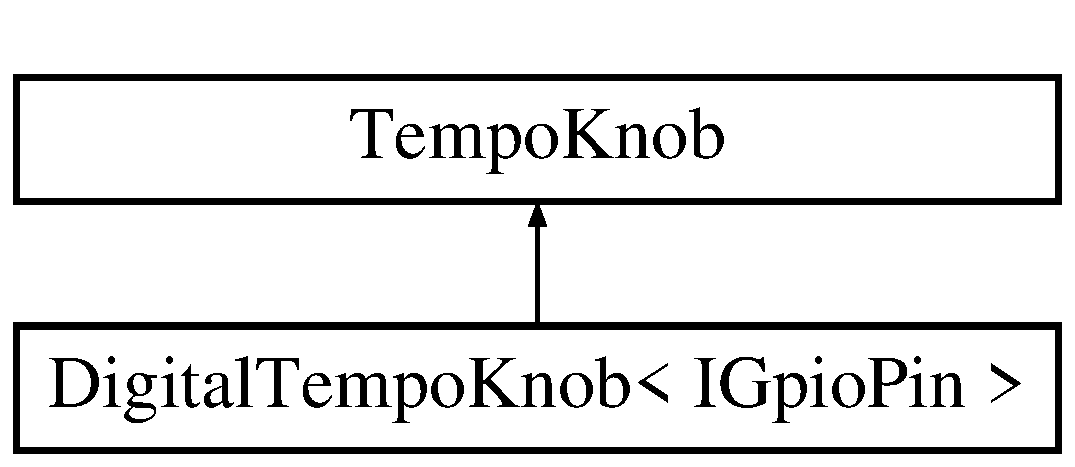
\includegraphics[height=2.000000cm]{class_digital_tempo_knob}
\end{center}
\end{figure}
\subsection*{Public Member Functions}
\begin{DoxyCompactItemize}
\item 
\mbox{\Hypertarget{class_digital_tempo_knob_a7a0c8f6a062484a035b37148beb591db}\label{class_digital_tempo_knob_a7a0c8f6a062484a035b37148beb591db}} 
{\bfseries Digital\+Tempo\+Knob} (\mbox{\hyperlink{class_rotary_encoder}{Rotary\+Encoder}}$<$ \mbox{\hyperlink{class_i_gpio_pin}{I\+Gpio\+Pin}} $>$ \&rotary\+Encoder)
\item 
\mbox{\Hypertarget{class_digital_tempo_knob_a3de50e157858cf898fd6c302575d06f7}\label{class_digital_tempo_knob_a3de50e157858cf898fd6c302575d06f7}} 
void {\bfseries set\+Reference\+Tempo} (u8 bpm)
\item 
\mbox{\Hypertarget{class_digital_tempo_knob_a3ab91bdef9c4f23e5b30e2dbb80500b3}\label{class_digital_tempo_knob_a3ab91bdef9c4f23e5b30e2dbb80500b3}} 
\mbox{\hyperlink{class_beats_per_minute}{Beats\+Per\+Minute}} {\bfseries read} () const final
\end{DoxyCompactItemize}


The documentation for this class was generated from the following files\+:\begin{DoxyCompactItemize}
\item 
..\textbackslash{}..\textbackslash{}software/presentation/tempo\+\_\+control/tempo\+\_\+knob/inc/digital\+\_\+tempo\+\_\+knob.\+h\item 
..\textbackslash{}..\textbackslash{}software/presentation/tempo\+\_\+control/tempo\+\_\+knob/src/digital\+\_\+tempo\+\_\+knob.\+cpp\end{DoxyCompactItemize}

\hypertarget{class_digital_tempo_knob_test}{}\section{Digital\+Tempo\+Knob\+Test Class Reference}
\label{class_digital_tempo_knob_test}\index{Digital\+Tempo\+Knob\+Test@{Digital\+Tempo\+Knob\+Test}}
Inheritance diagram for Digital\+Tempo\+Knob\+Test\+:\begin{figure}[H]
\begin{center}
\leavevmode
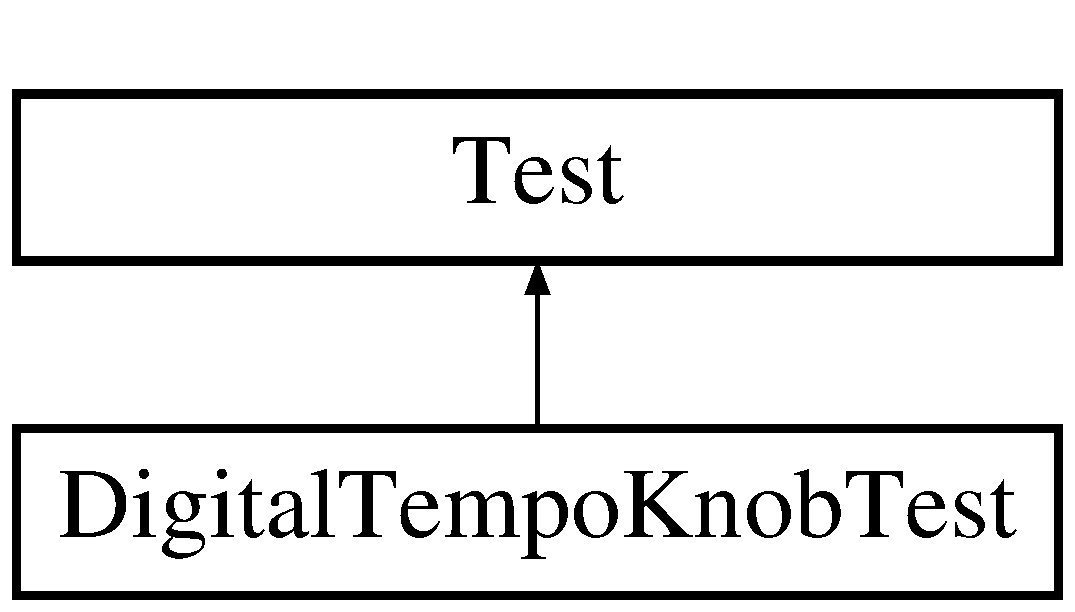
\includegraphics[height=2.000000cm]{class_digital_tempo_knob_test}
\end{center}
\end{figure}
\subsection*{Public Member Functions}
\begin{DoxyCompactItemize}
\item 
\mbox{\Hypertarget{class_digital_tempo_knob_test_aae7be94aeaa13fee37e7406fd2617886}\label{class_digital_tempo_knob_test_aae7be94aeaa13fee37e7406fd2617886}} 
void {\bfseries increase\+Mock\+Knob\+Rotations} ()
\item 
\mbox{\Hypertarget{class_digital_tempo_knob_test_a99015e4f13c986a9c6ac619c7b0ad9ce}\label{class_digital_tempo_knob_test_a99015e4f13c986a9c6ac619c7b0ad9ce}} 
void {\bfseries decrease\+Mock\+Knob\+Rotations} ()
\end{DoxyCompactItemize}
\subsection*{Public Attributes}
\begin{DoxyCompactItemize}
\item 
\mbox{\Hypertarget{class_digital_tempo_knob_test_a19d0db64dfb498356b8abb78c6992c80}\label{class_digital_tempo_knob_test_a19d0db64dfb498356b8abb78c6992c80}} 
\mbox{\hyperlink{class_gpio_pin_mock}{Gpio\+Pin\+Mock}} {\bfseries pinA}
\item 
\mbox{\Hypertarget{class_digital_tempo_knob_test_a22f3392dbcacb2b0ed639543776eba55}\label{class_digital_tempo_knob_test_a22f3392dbcacb2b0ed639543776eba55}} 
\mbox{\hyperlink{class_gpio_pin_mock}{Gpio\+Pin\+Mock}} {\bfseries pinB}
\item 
\mbox{\Hypertarget{class_digital_tempo_knob_test_ad7b5c9ecbdd01609c42686ee1a7545cf}\label{class_digital_tempo_knob_test_ad7b5c9ecbdd01609c42686ee1a7545cf}} 
\mbox{\hyperlink{class_rotary_encoder}{Rotary\+Encoder}}$<$ \mbox{\hyperlink{class_gpio_pin_mock}{Gpio\+Pin\+Mock}} $>$ {\bfseries encoder} = \mbox{\hyperlink{class_rotary_encoder}{Rotary\+Encoder}}$<$\mbox{\hyperlink{class_gpio_pin_mock}{Gpio\+Pin\+Mock}}$>$(pinA, pinB)
\item 
\mbox{\Hypertarget{class_digital_tempo_knob_test_a15b9dee201553e773b8490cf44b3b9f5}\label{class_digital_tempo_knob_test_a15b9dee201553e773b8490cf44b3b9f5}} 
\mbox{\hyperlink{class_digital_tempo_knob}{Digital\+Tempo\+Knob}}$<$ \mbox{\hyperlink{class_gpio_pin_mock}{Gpio\+Pin\+Mock}} $>$ {\bfseries knob} = \mbox{\hyperlink{class_digital_tempo_knob}{Digital\+Tempo\+Knob}}$<$\mbox{\hyperlink{class_gpio_pin_mock}{Gpio\+Pin\+Mock}}$>$(encoder)
\end{DoxyCompactItemize}


The documentation for this class was generated from the following file\+:\begin{DoxyCompactItemize}
\item 
..\textbackslash{}..\textbackslash{}software/presentation/tempo\+\_\+control/tempo\+\_\+knob/test/digital\+\_\+tempo\+\_\+knob\+\_\+test.\+cpp\end{DoxyCompactItemize}

\hypertarget{class_four_digit_display}{}\section{Four\+Digit\+Display Class Reference}
\label{class_four_digit_display}\index{Four\+Digit\+Display@{Four\+Digit\+Display}}
Inheritance diagram for Four\+Digit\+Display\+:\begin{figure}[H]
\begin{center}
\leavevmode
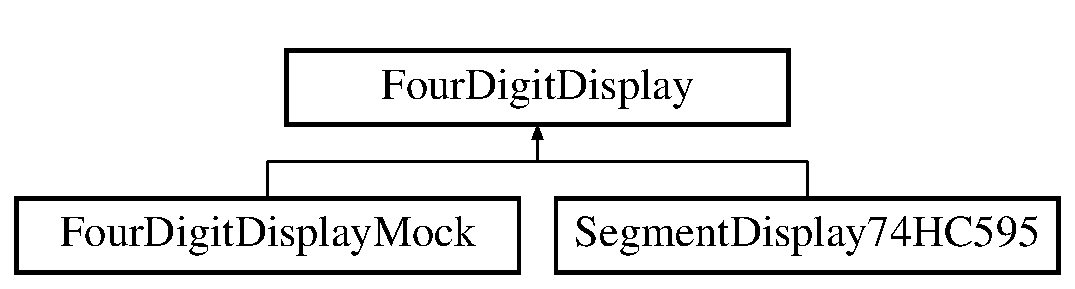
\includegraphics[height=2.000000cm]{class_four_digit_display}
\end{center}
\end{figure}
\subsection*{Public Member Functions}
\begin{DoxyCompactItemize}
\item 
\mbox{\Hypertarget{class_four_digit_display_a32ca43d20e2253ff51a1b23700c4cb13}\label{class_four_digit_display_a32ca43d20e2253ff51a1b23700c4cb13}} 
virtual void {\bfseries set\+Number\+To\+Display} (u16 number)=0
\item 
\mbox{\Hypertarget{class_four_digit_display_af6258c4601f0f028025a7a0c4905b79b}\label{class_four_digit_display_af6258c4601f0f028025a7a0c4905b79b}} 
virtual void {\bfseries enable\+Decimal\+Point} (u8 digit)=0
\item 
\mbox{\Hypertarget{class_four_digit_display_ac06686283c5486b98f95c32603b15662}\label{class_four_digit_display_ac06686283c5486b98f95c32603b15662}} 
virtual void {\bfseries disable\+Decimal\+Point} (u8 digit)=0
\end{DoxyCompactItemize}


The documentation for this class was generated from the following file\+:\begin{DoxyCompactItemize}
\item 
..\textbackslash{}..\textbackslash{}software/hal/if/fourdigitdisplay.\+h\end{DoxyCompactItemize}

\hypertarget{class_four_digit_display_mock}{}\section{Four\+Digit\+Display\+Mock Class Reference}
\label{class_four_digit_display_mock}\index{FourDigitDisplayMock@{FourDigitDisplayMock}}
Inheritance diagram for Four\+Digit\+Display\+Mock\+:\begin{figure}[H]
\begin{center}
\leavevmode
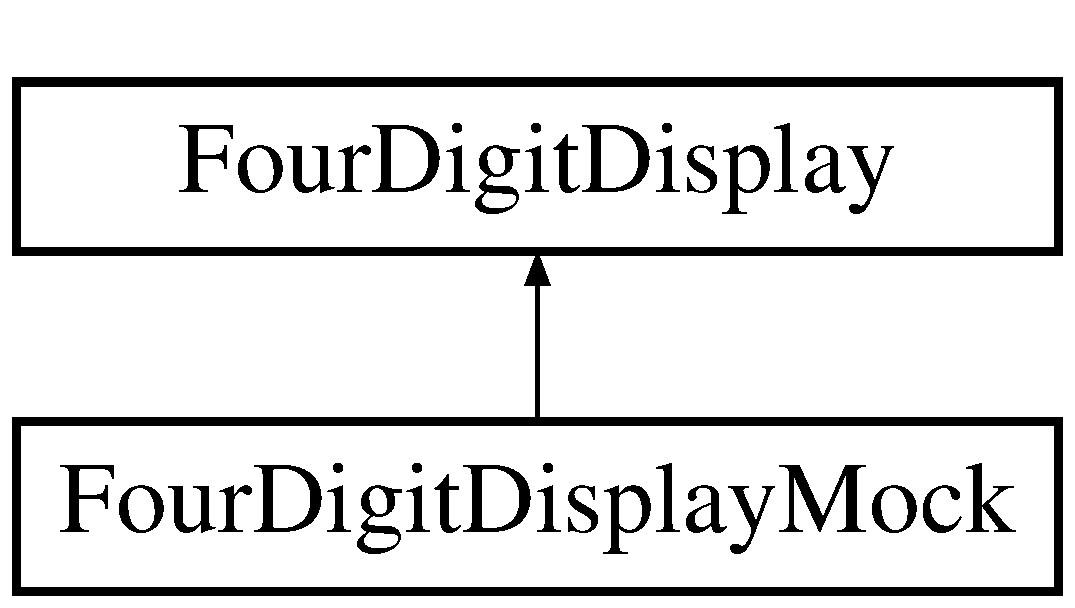
\includegraphics[height=2.000000cm]{class_four_digit_display_mock}
\end{center}
\end{figure}
\subsection*{Public Member Functions}
\begin{DoxyCompactItemize}
\item 
\mbox{\Hypertarget{class_four_digit_display_mock_ab597d895ae1f604eb0dd0e8d7920c743}\label{class_four_digit_display_mock_ab597d895ae1f604eb0dd0e8d7920c743}} 
{\bfseries M\+O\+C\+K\+\_\+\+M\+E\+T\+H\+O\+D1} (set\+Number\+To\+Display, void(u16 number))
\item 
\mbox{\Hypertarget{class_four_digit_display_mock_a11fcce7703bbb5d7b13eb4dcbdcb15fe}\label{class_four_digit_display_mock_a11fcce7703bbb5d7b13eb4dcbdcb15fe}} 
{\bfseries M\+O\+C\+K\+\_\+\+M\+E\+T\+H\+O\+D1} (enable\+Decimal\+Point, void(u8 digit))
\item 
\mbox{\Hypertarget{class_four_digit_display_mock_aaa591f57311085358e7a17e22b057b90}\label{class_four_digit_display_mock_aaa591f57311085358e7a17e22b057b90}} 
{\bfseries M\+O\+C\+K\+\_\+\+M\+E\+T\+H\+O\+D1} (disable\+Decimal\+Point, void(u8 digit))
\end{DoxyCompactItemize}


The documentation for this class was generated from the following file\+:\begin{DoxyCompactItemize}
\item 
C\+:/\+Development/code/proj/tr2k\+\_\+drum\+\_\+machine/software/hal/if/mock/Four\+Digit\+Display\+Mock.\+h\end{DoxyCompactItemize}

\hypertarget{class_gpio_pin}{}\section{Gpio\+Pin Class Reference}
\label{class_gpio_pin}\index{Gpio\+Pin@{Gpio\+Pin}}
Inheritance diagram for Gpio\+Pin\+:\begin{figure}[H]
\begin{center}
\leavevmode
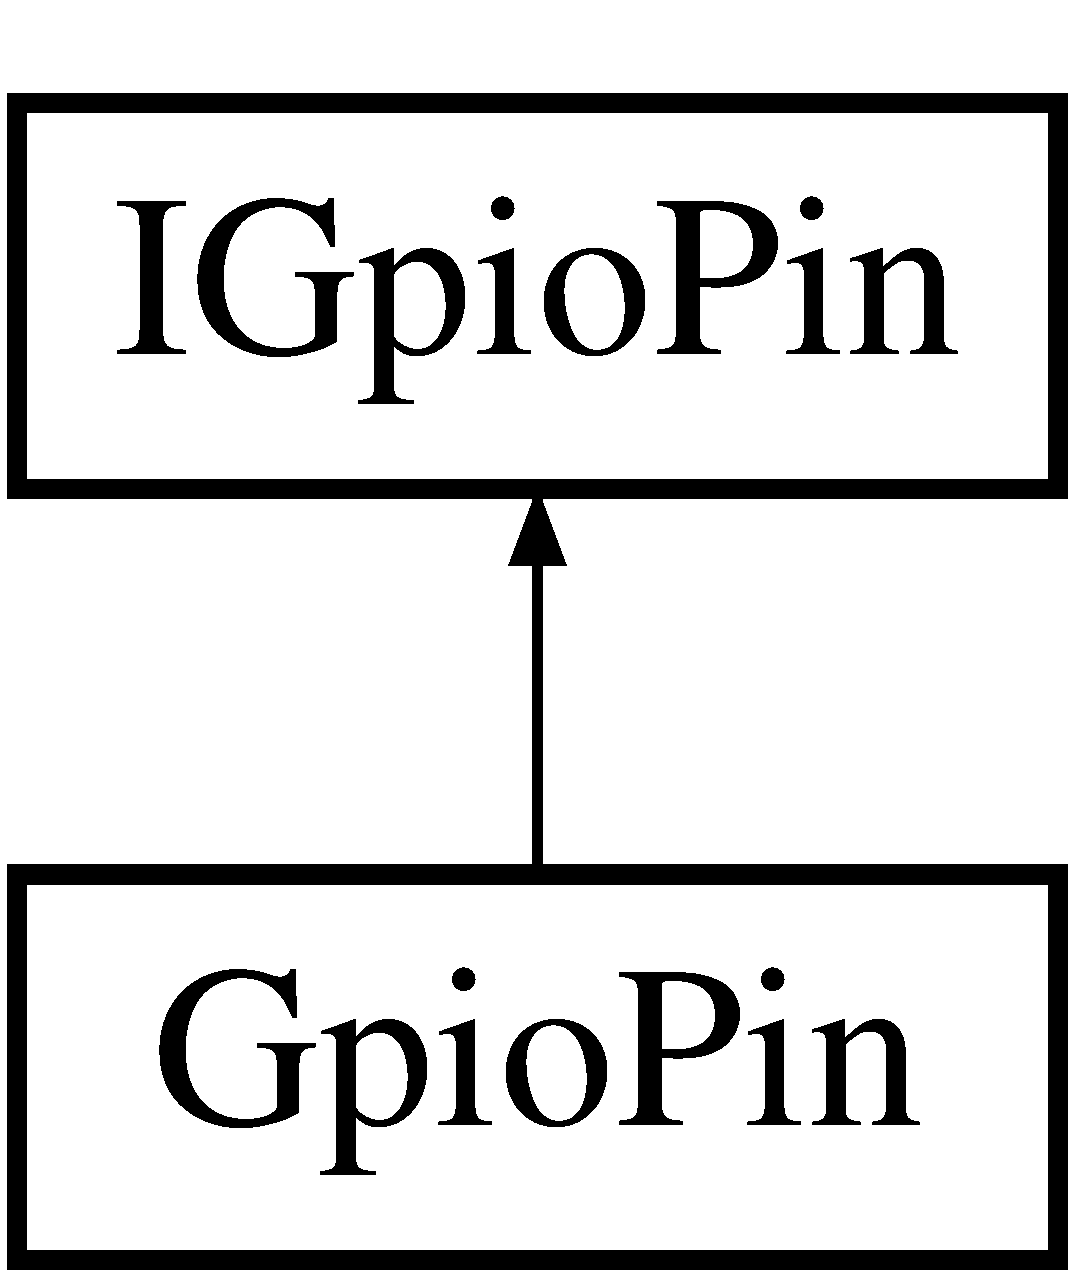
\includegraphics[height=2.000000cm]{class_gpio_pin}
\end{center}
\end{figure}
\subsection*{Public Member Functions}
\begin{DoxyCompactItemize}
\item 
\mbox{\Hypertarget{class_gpio_pin_a823123512552fe7226d12aeccccbdf6b}\label{class_gpio_pin_a823123512552fe7226d12aeccccbdf6b}} 
{\bfseries Gpio\+Pin} (Pin\+Number num, Port port)
\item 
\mbox{\Hypertarget{class_gpio_pin_a1da774161af27f3b9a0df07c5fa55fcd}\label{class_gpio_pin_a1da774161af27f3b9a0df07c5fa55fcd}} 
{\bfseries Gpio\+Pin} (Pin\+Number num, Port port, Data\+Direction dir)
\item 
\mbox{\Hypertarget{class_gpio_pin_ae09d7d1ef774b3dfee5cdaee5bf9a812}\label{class_gpio_pin_ae09d7d1ef774b3dfee5cdaee5bf9a812}} 
void {\bfseries set} ()
\item 
\mbox{\Hypertarget{class_gpio_pin_ad45c67b3ac159ad8d133317062e351e9}\label{class_gpio_pin_ad45c67b3ac159ad8d133317062e351e9}} 
void {\bfseries clear} ()
\item 
\mbox{\Hypertarget{class_gpio_pin_a43e55b13c02d838f5e2aa6ead319b7f6}\label{class_gpio_pin_a43e55b13c02d838f5e2aa6ead319b7f6}} 
void {\bfseries toggle} ()
\item 
\mbox{\Hypertarget{class_gpio_pin_a868ffd43b97af4082b43ab55794d8e9f}\label{class_gpio_pin_a868ffd43b97af4082b43ab55794d8e9f}} 
void {\bfseries write} (Logic\+State)
\item 
\mbox{\Hypertarget{class_gpio_pin_aae6ba33229b5237d943f1be6481164ef}\label{class_gpio_pin_aae6ba33229b5237d943f1be6481164ef}} 
Logic\+State {\bfseries read} ()
\item 
\mbox{\Hypertarget{class_gpio_pin_a0aef9e6efb8f955e07b6715a0801e51e}\label{class_gpio_pin_a0aef9e6efb8f955e07b6715a0801e51e}} 
void {\bfseries set\+Direction} (Data\+Direction direction)
\item 
\mbox{\Hypertarget{class_gpio_pin_a721e97dfff89d09add23ae80ab869254}\label{class_gpio_pin_a721e97dfff89d09add23ae80ab869254}} 
void {\bfseries set\+Input\+Register} (u8 \&regptr)
\item 
\mbox{\Hypertarget{class_gpio_pin_a0d12e95670d4426f50c419d9f6c2f954}\label{class_gpio_pin_a0d12e95670d4426f50c419d9f6c2f954}} 
void {\bfseries set\+Output\+Register} (u8 \&regptr)
\item 
\mbox{\Hypertarget{class_gpio_pin_a5389818286140e64e2383a4c2edacf63}\label{class_gpio_pin_a5389818286140e64e2383a4c2edacf63}} 
void {\bfseries set\+Data\+Direction\+Register} (u8 \&regptr)
\end{DoxyCompactItemize}


The documentation for this class was generated from the following files\+:\begin{DoxyCompactItemize}
\item 
..\textbackslash{}..\textbackslash{}software/drivers/gpio/inc/gpiopin.\+h\item 
..\textbackslash{}..\textbackslash{}software/drivers/gpio/src/gpiopin.\+cpp\end{DoxyCompactItemize}

\hypertarget{class_gpio_pin_mock}{}\section{Gpio\+Pin\+Mock Class Reference}
\label{class_gpio_pin_mock}\index{Gpio\+Pin\+Mock@{Gpio\+Pin\+Mock}}
Inheritance diagram for Gpio\+Pin\+Mock\+:\begin{figure}[H]
\begin{center}
\leavevmode
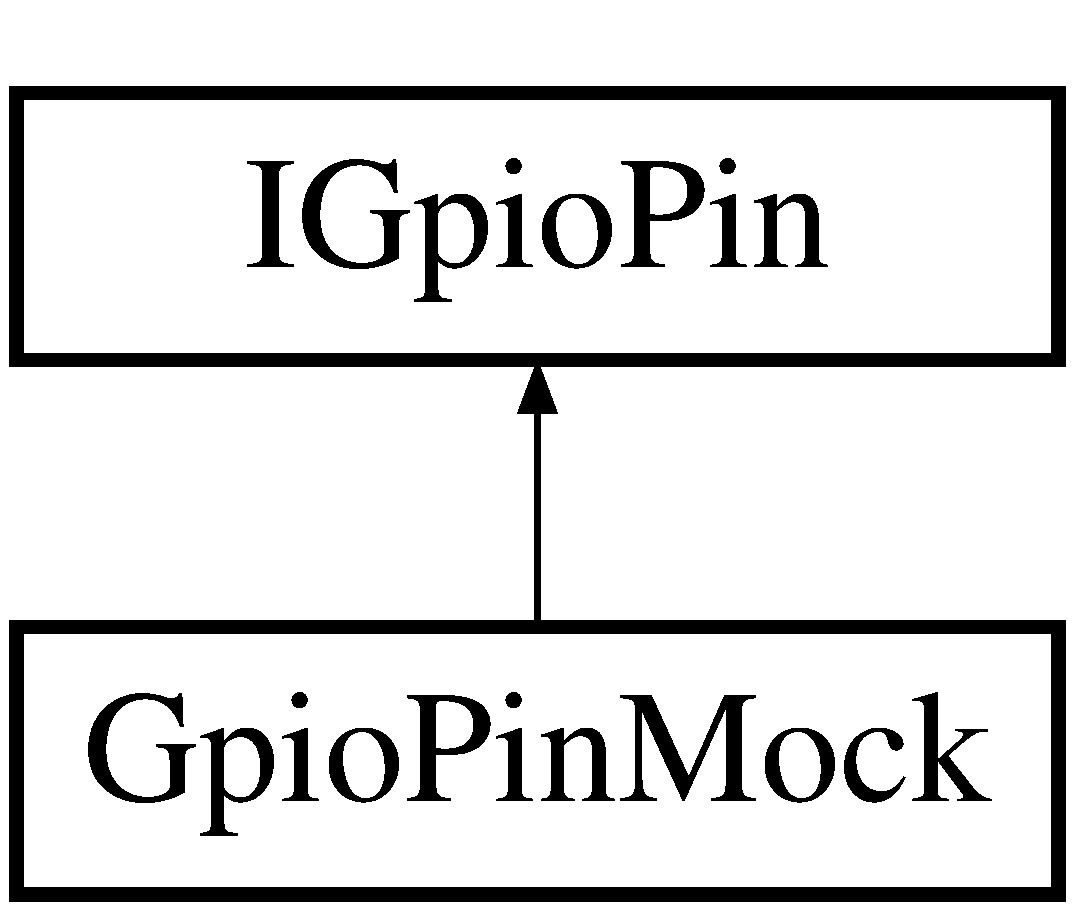
\includegraphics[height=2.000000cm]{class_gpio_pin_mock}
\end{center}
\end{figure}
\subsection*{Public Member Functions}
\begin{DoxyCompactItemize}
\item 
\mbox{\Hypertarget{class_gpio_pin_mock_a56f146c2b2a2bae6fd4cefb9d152b713}\label{class_gpio_pin_mock_a56f146c2b2a2bae6fd4cefb9d152b713}} 
{\bfseries M\+O\+C\+K\+\_\+\+M\+E\+T\+H\+O\+D0} (set, void())
\item 
\mbox{\Hypertarget{class_gpio_pin_mock_aa8fbc0b168892c31b9f2fa8f7b441fb8}\label{class_gpio_pin_mock_aa8fbc0b168892c31b9f2fa8f7b441fb8}} 
{\bfseries M\+O\+C\+K\+\_\+\+M\+E\+T\+H\+O\+D0} (clear, void())
\item 
\mbox{\Hypertarget{class_gpio_pin_mock_a360e0ac070c5fc973837f202d09231b8}\label{class_gpio_pin_mock_a360e0ac070c5fc973837f202d09231b8}} 
{\bfseries M\+O\+C\+K\+\_\+\+M\+E\+T\+H\+O\+D0} (toggle, void())
\item 
\mbox{\Hypertarget{class_gpio_pin_mock_a70637e5cff06f90e89abf1bea0af5f1b}\label{class_gpio_pin_mock_a70637e5cff06f90e89abf1bea0af5f1b}} 
{\bfseries M\+O\+C\+K\+\_\+\+M\+E\+T\+H\+O\+D1} (write, void(Logic\+State))
\item 
\mbox{\Hypertarget{class_gpio_pin_mock_a782457feb32b410b8bf159adf6f51527}\label{class_gpio_pin_mock_a782457feb32b410b8bf159adf6f51527}} 
{\bfseries M\+O\+C\+K\+\_\+\+M\+E\+T\+H\+O\+D0} (read, Logic\+State())
\item 
\mbox{\Hypertarget{class_gpio_pin_mock_ae9c2e1480c656283b64271eb6aca67a7}\label{class_gpio_pin_mock_ae9c2e1480c656283b64271eb6aca67a7}} 
{\bfseries M\+O\+C\+K\+\_\+\+M\+E\+T\+H\+O\+D1} (set\+Direction, void(Data\+Direction direction))
\end{DoxyCompactItemize}


The documentation for this class was generated from the following file\+:\begin{DoxyCompactItemize}
\item 
..\textbackslash{}..\textbackslash{}software/drivers/gpio/if/mock/igpiopin\+\_\+mock.\+h\end{DoxyCompactItemize}

\hypertarget{class_i_gpio_pin}{}\section{I\+Gpio\+Pin Class Reference}
\label{class_i_gpio_pin}\index{I\+Gpio\+Pin@{I\+Gpio\+Pin}}
Inheritance diagram for I\+Gpio\+Pin\+:\begin{figure}[H]
\begin{center}
\leavevmode
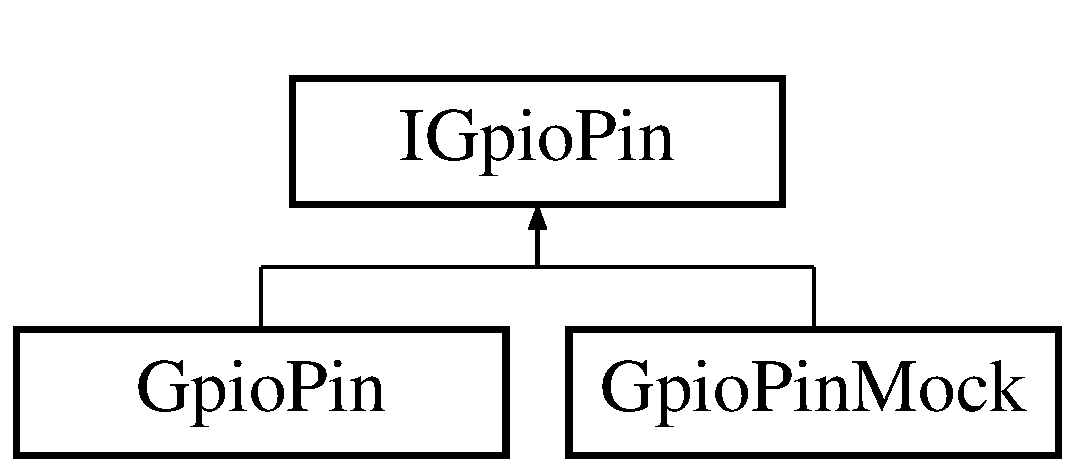
\includegraphics[height=2.000000cm]{class_i_gpio_pin}
\end{center}
\end{figure}
\subsection*{Public Member Functions}
\begin{DoxyCompactItemize}
\item 
\mbox{\Hypertarget{class_i_gpio_pin_aba7fc6b02a422e589f59265531b55d9a}\label{class_i_gpio_pin_aba7fc6b02a422e589f59265531b55d9a}} 
virtual void {\bfseries set} ()=0
\item 
\mbox{\Hypertarget{class_i_gpio_pin_af51fe6fdf248e4d1a114b72a8dc4e19d}\label{class_i_gpio_pin_af51fe6fdf248e4d1a114b72a8dc4e19d}} 
virtual void {\bfseries clear} ()=0
\item 
\mbox{\Hypertarget{class_i_gpio_pin_a1d068ad689c3d5044c91b6bb3ad63bce}\label{class_i_gpio_pin_a1d068ad689c3d5044c91b6bb3ad63bce}} 
virtual void {\bfseries toggle} ()=0
\item 
\mbox{\Hypertarget{class_i_gpio_pin_a47200f748224d9a66dc1e7205a43ea20}\label{class_i_gpio_pin_a47200f748224d9a66dc1e7205a43ea20}} 
virtual void {\bfseries write} (Logic\+State)=0
\item 
\mbox{\Hypertarget{class_i_gpio_pin_a17d8a4224c3317f9c211ed12dfc54126}\label{class_i_gpio_pin_a17d8a4224c3317f9c211ed12dfc54126}} 
virtual Logic\+State {\bfseries read} ()=0
\item 
\mbox{\Hypertarget{class_i_gpio_pin_a4054e58e8681fb028601c72ecd8cd652}\label{class_i_gpio_pin_a4054e58e8681fb028601c72ecd8cd652}} 
virtual void {\bfseries set\+Direction} (Data\+Direction direction)=0
\end{DoxyCompactItemize}


The documentation for this class was generated from the following file\+:\begin{DoxyCompactItemize}
\item 
..\textbackslash{}..\textbackslash{}software/drivers/gpio/if/igpiopin.\+h\end{DoxyCompactItemize}

\hypertarget{classr2k_1_1ivector}{}\section{r2k\+::ivector$<$ T $>$ Class Template Reference}
\label{classr2k_1_1ivector}\index{r2k::ivector$<$ T $>$@{r2k::ivector$<$ T $>$}}
Inheritance diagram for r2k\+::ivector$<$ T $>$\+:\begin{figure}[H]
\begin{center}
\leavevmode
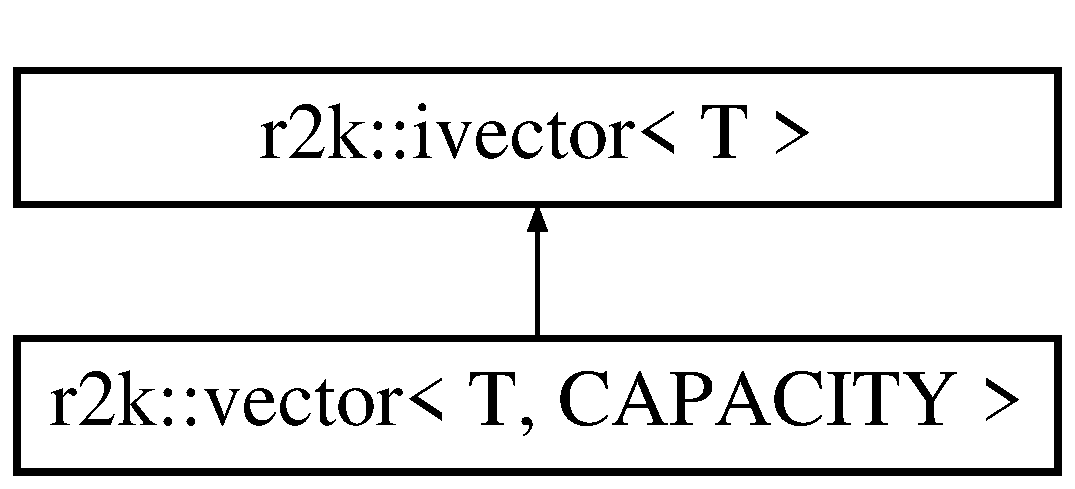
\includegraphics[height=2.000000cm]{classr2k_1_1ivector}
\end{center}
\end{figure}
\subsection*{Public Types}
\begin{DoxyCompactItemize}
\item 
\mbox{\Hypertarget{classr2k_1_1ivector_a3a4a70de708c8da5839e8ee768c98b5f}\label{classr2k_1_1ivector_a3a4a70de708c8da5839e8ee768c98b5f}} 
using {\bfseries value\+\_\+type} = T
\item 
\mbox{\Hypertarget{classr2k_1_1ivector_ace2102b41173217afd12cea873393cf2}\label{classr2k_1_1ivector_ace2102b41173217afd12cea873393cf2}} 
using {\bfseries iterator} = T $\ast$
\item 
\mbox{\Hypertarget{classr2k_1_1ivector_a516031d9abc36627e05a7291819ae73b}\label{classr2k_1_1ivector_a516031d9abc36627e05a7291819ae73b}} 
using {\bfseries reference} = T \&
\item 
\mbox{\Hypertarget{classr2k_1_1ivector_ad2d0d8eec97c5e73db7afcb5dc3d444a}\label{classr2k_1_1ivector_ad2d0d8eec97c5e73db7afcb5dc3d444a}} 
using {\bfseries const\+\_\+reference} = const T \&
\end{DoxyCompactItemize}
\subsection*{Public Member Functions}
\begin{DoxyCompactItemize}
\item 
\mbox{\Hypertarget{classr2k_1_1ivector_aa12c372c0503ee0f44686552673ef196}\label{classr2k_1_1ivector_aa12c372c0503ee0f44686552673ef196}} 
virtual iterator {\bfseries begin} ()=0
\item 
\mbox{\Hypertarget{classr2k_1_1ivector_a3f135257b47c1be208937eda8e28c2fc}\label{classr2k_1_1ivector_a3f135257b47c1be208937eda8e28c2fc}} 
virtual iterator {\bfseries end} ()=0
\item 
\mbox{\Hypertarget{classr2k_1_1ivector_a6b3b9b7efad8ae22e7e66105622fcb7f}\label{classr2k_1_1ivector_a6b3b9b7efad8ae22e7e66105622fcb7f}} 
virtual size\+\_\+t {\bfseries size} () const =0
\item 
\mbox{\Hypertarget{classr2k_1_1ivector_afed775f0a705c51683bc01a0b28f5f84}\label{classr2k_1_1ivector_afed775f0a705c51683bc01a0b28f5f84}} 
virtual size\+\_\+t {\bfseries capacity} () const =0
\item 
\mbox{\Hypertarget{classr2k_1_1ivector_aacd84b901da083ef9967da23085841d8}\label{classr2k_1_1ivector_aacd84b901da083ef9967da23085841d8}} 
virtual void {\bfseries resize} (size\+\_\+t)=0
\item 
\mbox{\Hypertarget{classr2k_1_1ivector_a9254e80c621114b589a990f8c76e930a}\label{classr2k_1_1ivector_a9254e80c621114b589a990f8c76e930a}} 
virtual bool {\bfseries empty} () const =0
\item 
\mbox{\Hypertarget{classr2k_1_1ivector_a2f260ae445e62901bef166d2ba02d88d}\label{classr2k_1_1ivector_a2f260ae445e62901bef166d2ba02d88d}} 
virtual reference {\bfseries operator\mbox{[}$\,$\mbox{]}} (size\+\_\+t index)=0
\item 
\mbox{\Hypertarget{classr2k_1_1ivector_ae4cafbfcdd7dae88a7fab06e26ecb470}\label{classr2k_1_1ivector_ae4cafbfcdd7dae88a7fab06e26ecb470}} 
virtual reference {\bfseries back} ()=0
\item 
\mbox{\Hypertarget{classr2k_1_1ivector_aab84081f12ca539f11ae5027e9441882}\label{classr2k_1_1ivector_aab84081f12ca539f11ae5027e9441882}} 
virtual void {\bfseries push\+\_\+back} (const\+\_\+reference val)=0
\item 
\mbox{\Hypertarget{classr2k_1_1ivector_ab4565993d539642c5ae4cef03fd096a3}\label{classr2k_1_1ivector_ab4565993d539642c5ae4cef03fd096a3}} 
virtual void {\bfseries pop\+\_\+back} ()=0
\end{DoxyCompactItemize}


The documentation for this class was generated from the following file\+:\begin{DoxyCompactItemize}
\item 
C\+:/\+Development/code/proj/tr2k\+\_\+drum\+\_\+machine/software/common/if/r2k/ivector.\+h\end{DoxyCompactItemize}

\hypertarget{classr2k_vector_test}{}\section{r2k\+Vector\+Test Class Reference}
\label{classr2k_vector_test}\index{r2k\+Vector\+Test@{r2k\+Vector\+Test}}
Inheritance diagram for r2k\+Vector\+Test\+:\begin{figure}[H]
\begin{center}
\leavevmode
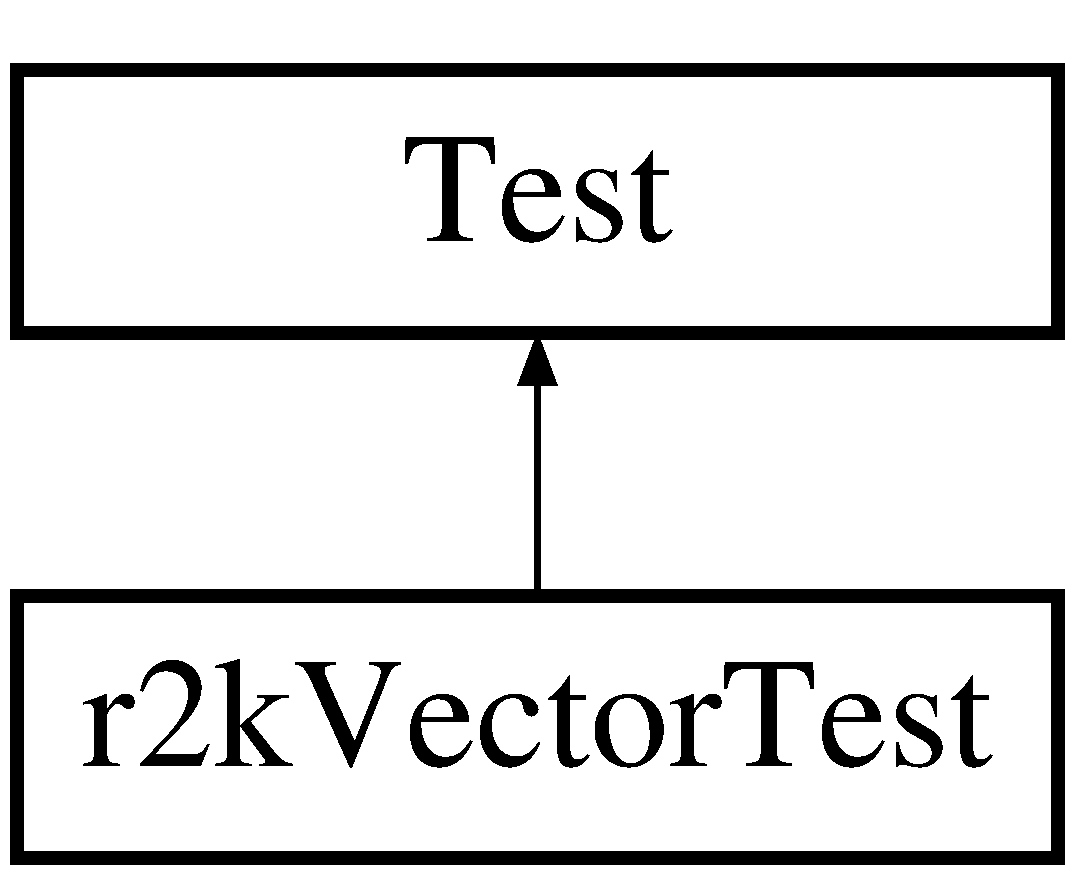
\includegraphics[height=2.000000cm]{classr2k_vector_test}
\end{center}
\end{figure}


The documentation for this class was generated from the following file\+:\begin{DoxyCompactItemize}
\item 
..\textbackslash{}..\textbackslash{}software/common/test/vector\+\_\+test.\+cpp\end{DoxyCompactItemize}

\hypertarget{class_rhythm_playback_controller}{}\section{Rhythm\+Playback\+Controller Class Reference}
\label{class_rhythm_playback_controller}\index{Rhythm\+Playback\+Controller@{Rhythm\+Playback\+Controller}}
\subsection*{Public Member Functions}
\begin{DoxyCompactItemize}
\item 
\mbox{\Hypertarget{class_rhythm_playback_controller_a9f280da7a6477eafe98fc4fc57b02a67}\label{class_rhythm_playback_controller_a9f280da7a6477eafe98fc4fc57b02a67}} 
{\bfseries Rhythm\+Playback\+Controller} (\mbox{\hyperlink{class_tempo_timer}{Tempo\+Timer}} \&timer)
\item 
\mbox{\Hypertarget{class_rhythm_playback_controller_ad61f44263753a449470b112870187060}\label{class_rhythm_playback_controller_ad61f44263753a449470b112870187060}} 
void {\bfseries set\+Tempo} (\mbox{\hyperlink{class_beats_per_minute}{Beats\+Per\+Minute}})
\item 
\mbox{\Hypertarget{class_rhythm_playback_controller_ad1c705dd42b2d91fb9171996fabbe507}\label{class_rhythm_playback_controller_ad1c705dd42b2d91fb9171996fabbe507}} 
void {\bfseries restart\+Playback} ()
\item 
\mbox{\Hypertarget{class_rhythm_playback_controller_a28db76a203bc7a143e37677cdf0ea602}\label{class_rhythm_playback_controller_a28db76a203bc7a143e37677cdf0ea602}} 
void {\bfseries stop\+Playback} ()
\item 
\mbox{\Hypertarget{class_rhythm_playback_controller_a651af2f689e72a3b3bc5e172e12a965c}\label{class_rhythm_playback_controller_a651af2f689e72a3b3bc5e172e12a965c}} 
void {\bfseries continue\+Playback} ()
\end{DoxyCompactItemize}


The documentation for this class was generated from the following files\+:\begin{DoxyCompactItemize}
\item 
..\textbackslash{}..\textbackslash{}software/application/rhythm\+\_\+playback\+\_\+controller/inc/rhythm\+\_\+playback\+\_\+controller.\+h\item 
..\textbackslash{}..\textbackslash{}software/application/rhythm\+\_\+playback\+\_\+controller/src/rhythm\+\_\+playback\+\_\+controller.\+cpp\end{DoxyCompactItemize}

\hypertarget{class_rotary_encoder}{}\section{Rotary\+Encoder$<$ I\+Gpio\+Pin $>$ Class Template Reference}
\label{class_rotary_encoder}\index{RotaryEncoder$<$ IGpioPin $>$@{RotaryEncoder$<$ IGpioPin $>$}}
\subsection*{Public Member Functions}
\begin{DoxyCompactItemize}
\item 
\mbox{\Hypertarget{class_rotary_encoder_a4dd277ba00fe46063f5778b202fa8414}\label{class_rotary_encoder_a4dd277ba00fe46063f5778b202fa8414}} 
{\bfseries Rotary\+Encoder} (\mbox{\hyperlink{class_i_gpio_pin}{I\+Gpio\+Pin}} \&pinA, \mbox{\hyperlink{class_i_gpio_pin}{I\+Gpio\+Pin}} \&pinB)
\item 
\mbox{\Hypertarget{class_rotary_encoder_af2d26ccf013052b3f223e40e0b4d6a9e}\label{class_rotary_encoder_af2d26ccf013052b3f223e40e0b4d6a9e}} 
void {\bfseries handle\+Edge} ()
\item 
\mbox{\Hypertarget{class_rotary_encoder_a0074aa5a32961e08fcd89871f303939c}\label{class_rotary_encoder_a0074aa5a32961e08fcd89871f303939c}} 
void {\bfseries set\+Rotation\+Ceiling} (s16)
\item 
\mbox{\Hypertarget{class_rotary_encoder_a04c456e6194eea6f69404243eff954af}\label{class_rotary_encoder_a04c456e6194eea6f69404243eff954af}} 
void {\bfseries set\+Rotation\+Floor} (s16)
\item 
\mbox{\Hypertarget{class_rotary_encoder_aa5e3039a73f78b6c323f061e03dd0f8d}\label{class_rotary_encoder_aa5e3039a73f78b6c323f061e03dd0f8d}} 
s16 {\bfseries get\+Num\+Rotations} ()
\end{DoxyCompactItemize}


The documentation for this class was generated from the following files\+:\begin{DoxyCompactItemize}
\item 
C\+:/\+Development/code/proj/tr2k\+\_\+drum\+\_\+machine/software/drivers/\+Rotary\+Encoder/inc/Rotary\+Encoder.\+h\item 
C\+:/\+Development/code/proj/tr2k\+\_\+drum\+\_\+machine/software/drivers/\+Rotary\+Encoder/src/Rotary\+Encoder.\+cpp\end{DoxyCompactItemize}

\hypertarget{class_rotary_encoder_test}{}\section{Rotary\+Encoder\+Test Class Reference}
\label{class_rotary_encoder_test}\index{Rotary\+Encoder\+Test@{Rotary\+Encoder\+Test}}
Inheritance diagram for Rotary\+Encoder\+Test\+:\begin{figure}[H]
\begin{center}
\leavevmode
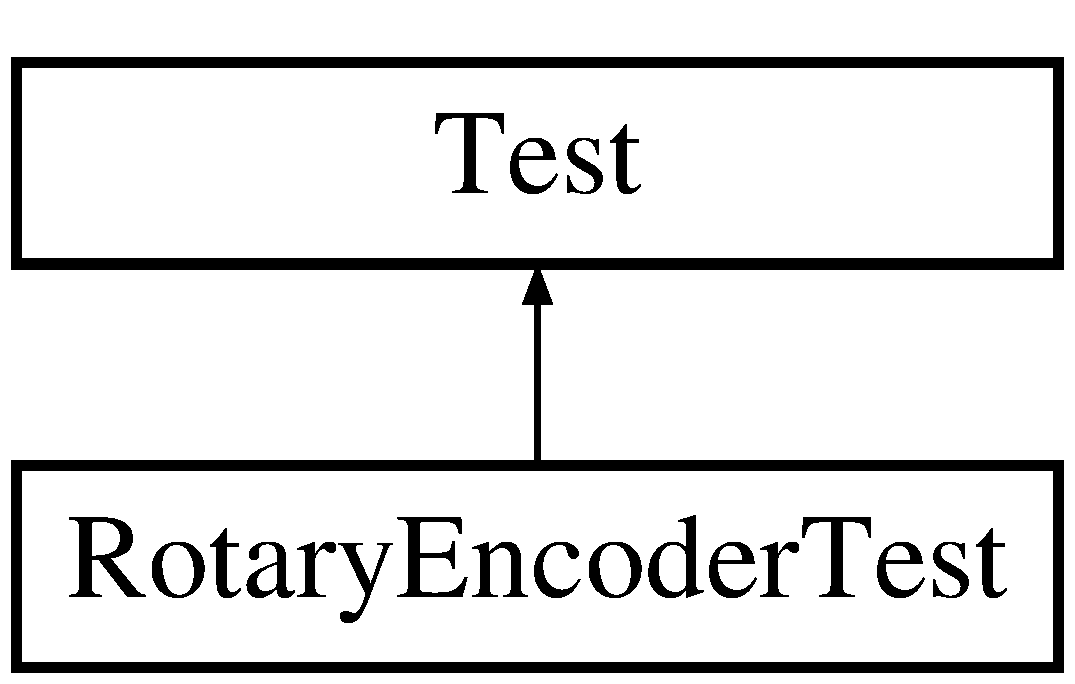
\includegraphics[height=2.000000cm]{class_rotary_encoder_test}
\end{center}
\end{figure}
\subsection*{Public Attributes}
\begin{DoxyCompactItemize}
\item 
\mbox{\Hypertarget{class_rotary_encoder_test_a8079cd19d6660966a63c83257a9bab2f}\label{class_rotary_encoder_test_a8079cd19d6660966a63c83257a9bab2f}} 
\mbox{\hyperlink{class_gpio_pin_mock}{Gpio\+Pin\+Mock}} {\bfseries pinA}
\item 
\mbox{\Hypertarget{class_rotary_encoder_test_af7150e74ea15ac798ff338d228e36995}\label{class_rotary_encoder_test_af7150e74ea15ac798ff338d228e36995}} 
\mbox{\hyperlink{class_gpio_pin_mock}{Gpio\+Pin\+Mock}} {\bfseries pinB}
\item 
\mbox{\Hypertarget{class_rotary_encoder_test_a88efb9449b23f19dba25f6e7e960b900}\label{class_rotary_encoder_test_a88efb9449b23f19dba25f6e7e960b900}} 
\mbox{\hyperlink{class_rotary_encoder}{Rotary\+Encoder}}$<$ \mbox{\hyperlink{class_gpio_pin_mock}{Gpio\+Pin\+Mock}} $>$ {\bfseries encoder} = \mbox{\hyperlink{class_rotary_encoder}{Rotary\+Encoder}}$<$\mbox{\hyperlink{class_gpio_pin_mock}{Gpio\+Pin\+Mock}}$>$(pinA, pinB)
\end{DoxyCompactItemize}


The documentation for this class was generated from the following file\+:\begin{DoxyCompactItemize}
\item 
..\textbackslash{}..\textbackslash{}software/drivers/rotary\+\_\+encoder/test/rotary\+\_\+encoder\+\_\+test.\+cpp\end{DoxyCompactItemize}

\hypertarget{class_segment_display74_h_c595}{}\section{Segment\+Display74\+H\+C595 Class Reference}
\label{class_segment_display74_h_c595}\index{SegmentDisplay74HC595@{SegmentDisplay74HC595}}
Inheritance diagram for Segment\+Display74\+H\+C595\+:\begin{figure}[H]
\begin{center}
\leavevmode
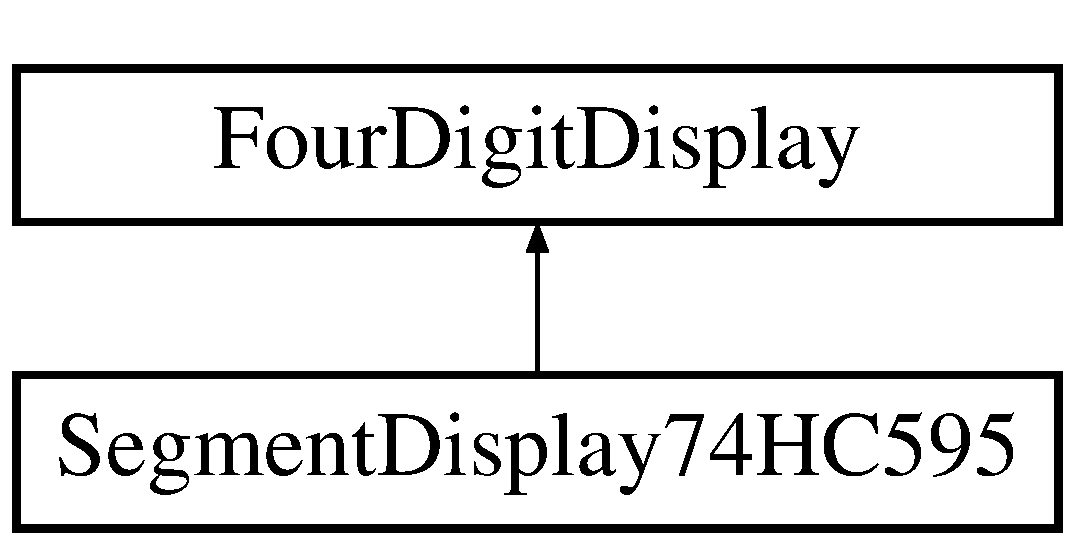
\includegraphics[height=2.000000cm]{class_segment_display74_h_c595}
\end{center}
\end{figure}
\subsection*{Public Member Functions}
\begin{DoxyCompactItemize}
\item 
\mbox{\Hypertarget{class_segment_display74_h_c595_ab5a35d882faf010f1f1d5b8f8314a838}\label{class_segment_display74_h_c595_ab5a35d882faf010f1f1d5b8f8314a838}} 
{\bfseries Segment\+Display74\+H\+C595} (\mbox{\hyperlink{class_spi}{Spi}} \&spi)
\item 
\mbox{\Hypertarget{class_segment_display74_h_c595_af3e2629cbe560a66a48e35d7cdb113fb}\label{class_segment_display74_h_c595_af3e2629cbe560a66a48e35d7cdb113fb}} 
void {\bfseries set\+Number\+To\+Display} (u16 number)
\item 
\mbox{\Hypertarget{class_segment_display74_h_c595_a8dc330ae5b1cc9d3b6a942fd4bbf891c}\label{class_segment_display74_h_c595_a8dc330ae5b1cc9d3b6a942fd4bbf891c}} 
void {\bfseries enable\+Decimal\+Point} (u8 digit)
\item 
\mbox{\Hypertarget{class_segment_display74_h_c595_a7c0153365c19a9e28e4b8ef43f11fa61}\label{class_segment_display74_h_c595_a7c0153365c19a9e28e4b8ef43f11fa61}} 
void {\bfseries disable\+Decimal\+Point} (u8 digit)
\item 
\mbox{\Hypertarget{class_segment_display74_h_c595_a06b400297778098161efbeee609fe8c2}\label{class_segment_display74_h_c595_a06b400297778098161efbeee609fe8c2}} 
void {\bfseries output\+Digit} (u8 digit)
\end{DoxyCompactItemize}


The documentation for this class was generated from the following files\+:\begin{DoxyCompactItemize}
\item 
C\+:/\+Development/code/proj/tr2k\+\_\+drum\+\_\+machine/software/drivers/\+Segment\+Display/inc/Segment\+Display.\+h\item 
C\+:/\+Development/code/proj/tr2k\+\_\+drum\+\_\+machine/software/drivers/\+Segment\+Display/src/Segment\+Display.\+cpp\end{DoxyCompactItemize}

\hypertarget{class_spi}{}\section{Spi Class Reference}
\label{class_spi}\index{Spi@{Spi}}
\subsection*{Public Member Functions}
\begin{DoxyCompactItemize}
\item 
\mbox{\hyperlink{class_spi_a27b7b236f911650839cf9465bfc4b972}{Spi}} ()
\item 
\mbox{\hyperlink{class_spi_aa5bff4855080ca494dda262669931973}{Spi}} (u8 \&pin\+Dir\+Reg, u8 \&control\+Reg, u8 \&stat\+Reg, u8 \&data\+Reg)
\item 
void \mbox{\hyperlink{class_spi_af36b174c9f4ab3dcd3d1b24587d396c8}{set\+Clock\+Speed}} (Spi\+Clock\+Speed)
\item 
void \mbox{\hyperlink{class_spi_aee3ca300877494f2c66be7c99d831ee1}{set\+Bit\+Order}} (Spi\+Bit\+Order)
\item 
void \mbox{\hyperlink{class_spi_af95597dbf2ad61755808ea6d87e587f1}{send\+Byte}} (u8 tx\+Byte)
\item 
void \mbox{\hyperlink{class_spi_a11ab7b1a91e22d08a43ae08d94ca447d}{set\+Tx\+Buffer}} (\mbox{\hyperlink{classr2k_1_1ivector}{r2k\+::ivector}}$<$ u8 $>$ \&buffer)
\item 
void \mbox{\hyperlink{class_spi_ad356e46ffdf7cc7d674eb871f05e8b0d}{send\+Next\+Byte\+In\+Buffer}} ()
\item 
bool \mbox{\hyperlink{class_spi_a8cf0289f4aaa9298b479a48de1dd6cb8}{tx\+Buffer\+Is\+Empty}} () const
\end{DoxyCompactItemize}


\subsection{Constructor \& Destructor Documentation}
\mbox{\Hypertarget{class_spi_a27b7b236f911650839cf9465bfc4b972}\label{class_spi_a27b7b236f911650839cf9465bfc4b972}} 
\index{Spi@{Spi}!Spi@{Spi}}
\index{Spi@{Spi}!Spi@{Spi}}
\subsubsection{\texorpdfstring{Spi()}{Spi()}\hspace{0.1cm}{\footnotesize\ttfamily [1/2]}}
{\footnotesize\ttfamily Spi\+::\+Spi (\begin{DoxyParamCaption}{ }\end{DoxyParamCaption})}

Constructor used in release build. \mbox{\Hypertarget{class_spi_aa5bff4855080ca494dda262669931973}\label{class_spi_aa5bff4855080ca494dda262669931973}} 
\index{Spi@{Spi}!Spi@{Spi}}
\index{Spi@{Spi}!Spi@{Spi}}
\subsubsection{\texorpdfstring{Spi()}{Spi()}\hspace{0.1cm}{\footnotesize\ttfamily [2/2]}}
{\footnotesize\ttfamily Spi\+::\+Spi (\begin{DoxyParamCaption}\item[{u8 \&}]{pin\+Dir\+Reg,  }\item[{u8 \&}]{control\+Reg,  }\item[{u8 \&}]{stat\+Reg,  }\item[{u8 \&}]{data\+Reg }\end{DoxyParamCaption})}

Constructor used in unit tests. 

\subsection{Member Function Documentation}
\mbox{\Hypertarget{class_spi_af95597dbf2ad61755808ea6d87e587f1}\label{class_spi_af95597dbf2ad61755808ea6d87e587f1}} 
\index{Spi@{Spi}!sendByte@{sendByte}}
\index{sendByte@{sendByte}!Spi@{Spi}}
\subsubsection{\texorpdfstring{sendByte()}{sendByte()}}
{\footnotesize\ttfamily void Spi\+::send\+Byte (\begin{DoxyParamCaption}\item[{u8}]{tx\+Byte }\end{DoxyParamCaption})}

Sends single byte over S\+PI in blocking mode, returns after transfer\textquotesingle{}s done. 
\begin{DoxyParams}{Parameters}
{\em byte} & to transfer. \\
\hline
\end{DoxyParams}
\mbox{\Hypertarget{class_spi_ad356e46ffdf7cc7d674eb871f05e8b0d}\label{class_spi_ad356e46ffdf7cc7d674eb871f05e8b0d}} 
\index{Spi@{Spi}!sendNextByteInBuffer@{sendNextByteInBuffer}}
\index{sendNextByteInBuffer@{sendNextByteInBuffer}!Spi@{Spi}}
\subsubsection{\texorpdfstring{sendNextByteInBuffer()}{sendNextByteInBuffer()}}
{\footnotesize\ttfamily void Spi\+::send\+Next\+Byte\+In\+Buffer (\begin{DoxyParamCaption}{ }\end{DoxyParamCaption})}

Sends the next byte in the tx\+Buffer and updates the byte index if buffer none-\/empty, otherwise sends a zero. \mbox{\Hypertarget{class_spi_aee3ca300877494f2c66be7c99d831ee1}\label{class_spi_aee3ca300877494f2c66be7c99d831ee1}} 
\index{Spi@{Spi}!setBitOrder@{setBitOrder}}
\index{setBitOrder@{setBitOrder}!Spi@{Spi}}
\subsubsection{\texorpdfstring{setBitOrder()}{setBitOrder()}}
{\footnotesize\ttfamily void Spi\+::set\+Bit\+Order (\begin{DoxyParamCaption}\item[{Spi\+Bit\+Order}]{order }\end{DoxyParamCaption})}

Determines what order to transmit bits, least significant bit first or most significant bit first. 
\begin{DoxyParams}{Parameters}
{\em enum} & determining L\+SB or M\+SB first. \\
\hline
\end{DoxyParams}
\mbox{\Hypertarget{class_spi_af36b174c9f4ab3dcd3d1b24587d396c8}\label{class_spi_af36b174c9f4ab3dcd3d1b24587d396c8}} 
\index{Spi@{Spi}!setClockSpeed@{setClockSpeed}}
\index{setClockSpeed@{setClockSpeed}!Spi@{Spi}}
\subsubsection{\texorpdfstring{setClockSpeed()}{setClockSpeed()}}
{\footnotesize\ttfamily void Spi\+::set\+Clock\+Speed (\begin{DoxyParamCaption}\item[{Spi\+Clock\+Speed}]{clock\+Speed }\end{DoxyParamCaption})}

Sets the speed of the serial clock used to drive the S\+PI slave by writing a number from a table to designated register bits.


\begin{DoxyParams}{Parameters}
{\em clock\+Speed} & selected with a prescaler for the system clock. \\
\hline
\end{DoxyParams}
\mbox{\Hypertarget{class_spi_a11ab7b1a91e22d08a43ae08d94ca447d}\label{class_spi_a11ab7b1a91e22d08a43ae08d94ca447d}} 
\index{Spi@{Spi}!setTxBuffer@{setTxBuffer}}
\index{setTxBuffer@{setTxBuffer}!Spi@{Spi}}
\subsubsection{\texorpdfstring{setTxBuffer()}{setTxBuffer()}}
{\footnotesize\ttfamily void Spi\+::set\+Tx\+Buffer (\begin{DoxyParamCaption}\item[{\mbox{\hyperlink{classr2k_1_1ivector}{r2k\+::ivector}}$<$ u8 $>$ \&}]{buffer }\end{DoxyParamCaption})}

Set a buffer of bytes to use for transferring data.

Note Bene\+: Use the \char`\"{}tx\+Buffer\+Is\+Empty\char`\"{}-\/method to check if more bytes need to be transfered, and transfer them using the \char`\"{}send\+Next\+Buffer\+Byte\char`\"{} method.


\begin{DoxyParams}{Parameters}
{\em buffer} & reference to byte buffer to transfer. \\
\hline
\end{DoxyParams}
\mbox{\Hypertarget{class_spi_a8cf0289f4aaa9298b479a48de1dd6cb8}\label{class_spi_a8cf0289f4aaa9298b479a48de1dd6cb8}} 
\index{Spi@{Spi}!txBufferIsEmpty@{txBufferIsEmpty}}
\index{txBufferIsEmpty@{txBufferIsEmpty}!Spi@{Spi}}
\subsubsection{\texorpdfstring{txBufferIsEmpty()}{txBufferIsEmpty()}}
{\footnotesize\ttfamily bool Spi\+::tx\+Buffer\+Is\+Empty (\begin{DoxyParamCaption}{ }\end{DoxyParamCaption}) const}

\begin{DoxyReturn}{Returns}
true if all bytes in tx buffer have ben transferred 
\end{DoxyReturn}


The documentation for this class was generated from the following files\+:\begin{DoxyCompactItemize}
\item 
C\+:/\+Development/code/proj/tr2k\+\_\+drum\+\_\+machine/software/drivers/\+Spi/inc/Spi.\+h\item 
C\+:/\+Development/code/proj/tr2k\+\_\+drum\+\_\+machine/software/drivers/\+Spi/src/Spi.\+cpp\end{DoxyCompactItemize}

\hypertarget{class_spi_test}{}\section{Spi\+Test Class Reference}
\label{class_spi_test}\index{Spi\+Test@{Spi\+Test}}
Inheritance diagram for Spi\+Test\+:\begin{figure}[H]
\begin{center}
\leavevmode
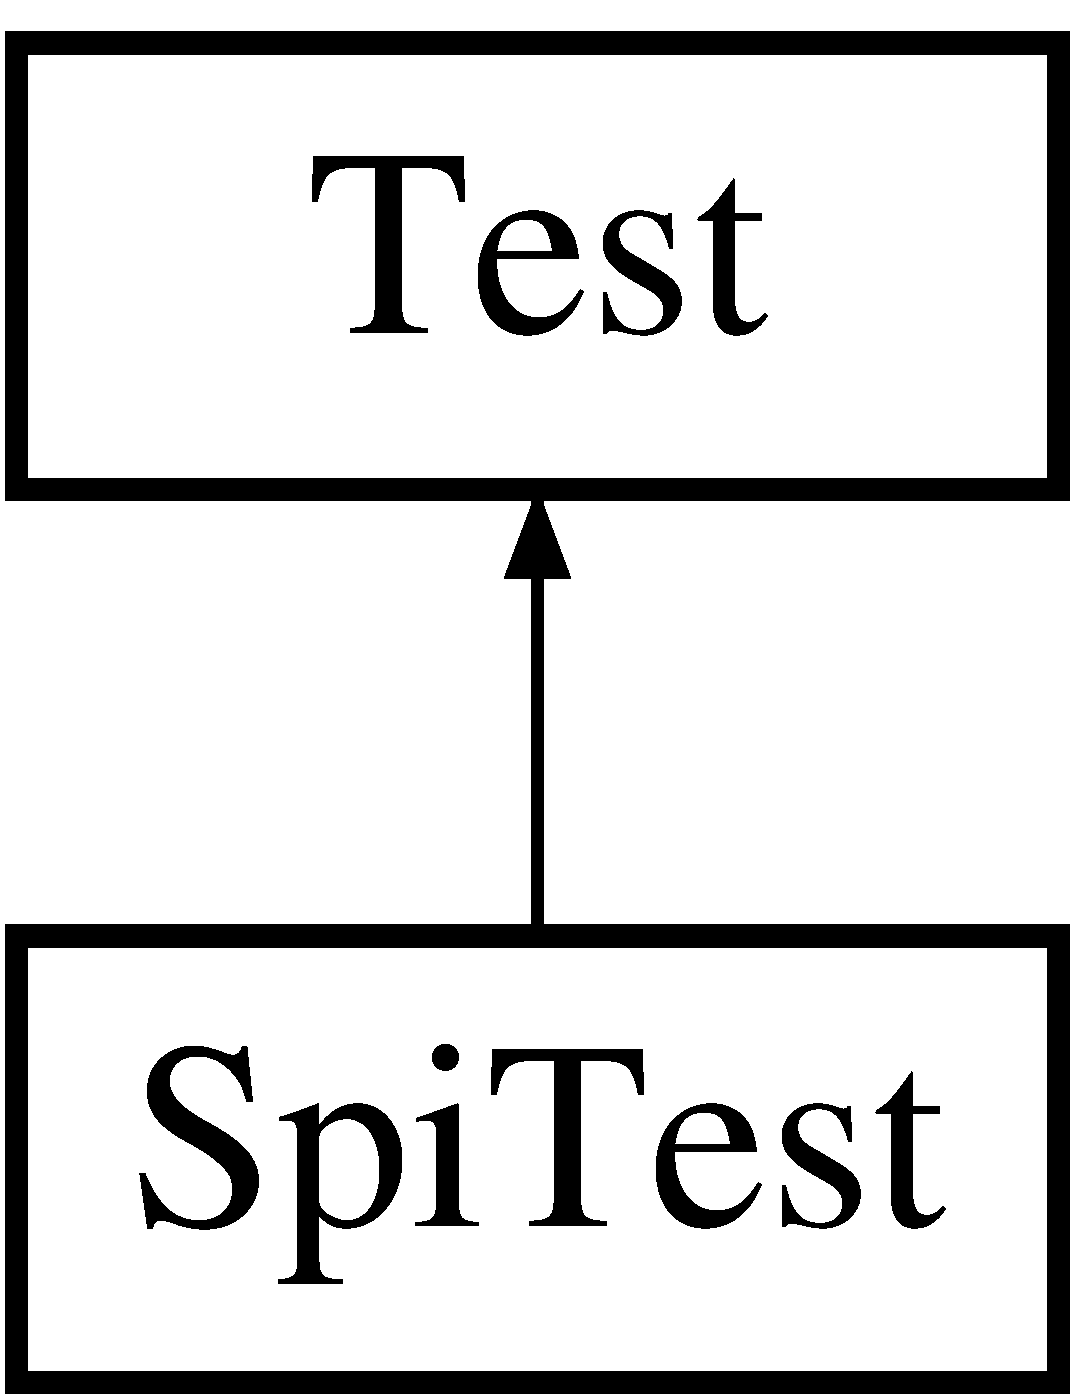
\includegraphics[height=2.000000cm]{class_spi_test}
\end{center}
\end{figure}
\subsection*{Public Member Functions}
\begin{DoxyCompactItemize}
\item 
u8 \mbox{\hyperlink{class_spi_test_a6f3260038241bf80545cddf4e1d73130}{get\+Clock\+Speed\+From\+Registers}} ()
\end{DoxyCompactItemize}
\subsection*{Public Attributes}
\begin{DoxyCompactItemize}
\item 
\mbox{\Hypertarget{class_spi_test_a2124422a4366e5d93c187f28b501d329}\label{class_spi_test_a2124422a4366e5d93c187f28b501d329}} 
u8 {\bfseries pin\+Direction\+Reg} = 0
\item 
\mbox{\Hypertarget{class_spi_test_a880e38b17b7c677f4bb8f080d9c456ce}\label{class_spi_test_a880e38b17b7c677f4bb8f080d9c456ce}} 
u8 {\bfseries control\+Reg} = 0
\item 
\mbox{\Hypertarget{class_spi_test_a699992d86eb612c5075cb6c20fbc7ee3}\label{class_spi_test_a699992d86eb612c5075cb6c20fbc7ee3}} 
u8 {\bfseries status\+Reg} = 0
\item 
\mbox{\Hypertarget{class_spi_test_aa67bba41833d0757d6d60f24102313bf}\label{class_spi_test_aa67bba41833d0757d6d60f24102313bf}} 
u8 {\bfseries data\+Reg} = 0
\item 
\mbox{\Hypertarget{class_spi_test_a2cb7044aa4c2cf119b0ee7338e0e66b6}\label{class_spi_test_a2cb7044aa4c2cf119b0ee7338e0e66b6}} 
\mbox{\hyperlink{class_spi}{Spi}} {\bfseries spi} = \mbox{\hyperlink{class_spi}{Spi}}(pin\+Direction\+Reg, control\+Reg, status\+Reg, data\+Reg)
\end{DoxyCompactItemize}


\subsection{Member Function Documentation}
\mbox{\Hypertarget{class_spi_test_a6f3260038241bf80545cddf4e1d73130}\label{class_spi_test_a6f3260038241bf80545cddf4e1d73130}} 
\index{Spi\+Test@{Spi\+Test}!get\+Clock\+Speed\+From\+Registers@{get\+Clock\+Speed\+From\+Registers}}
\index{get\+Clock\+Speed\+From\+Registers@{get\+Clock\+Speed\+From\+Registers}!Spi\+Test@{Spi\+Test}}
\subsubsection{\texorpdfstring{get\+Clock\+Speed\+From\+Registers()}{getClockSpeedFromRegisters()}}
{\footnotesize\ttfamily u8 Spi\+Test\+::get\+Clock\+Speed\+From\+Registers (\begin{DoxyParamCaption}{ }\end{DoxyParamCaption})\hspace{0.3cm}{\ttfamily [inline]}}

Combines bits S\+P\+R0, S\+P\+R1 and S\+P\+I2X to form the entries in table 23-\/5 \char`\"{}\+Relationship between S\+C\+K and Oscillator Frequency\char`\"{} at page 222 in the \char`\"{}\+Atmel-\/42735\+B-\/\+A\+Tmega328/\+P\+\_\+\+Datasheet\+\_\+\+Complete-\/11/2016\char`\"{} document.

\subsubsection*{Selection Number $\vert$ S\+PI Clock Frequency }

0 $\vert$ Sys Freq / 4 1 $\vert$ Sys Freq / 16 2 $\vert$ Sys Freq / 64 3 $\vert$ Sys Freq / 128 4 $\vert$ Sys Freq / 2 5 $\vert$ Sys Freq / 8 6 $\vert$ Sys Freq / 32 7 $\vert$ Sys Freq / 64 

The documentation for this class was generated from the following file\+:\begin{DoxyCompactItemize}
\item 
..\textbackslash{}..\textbackslash{}software/drivers/spi/test/spitest.\+cpp\end{DoxyCompactItemize}

\hypertarget{class_tempo_control_view}{}\section{Tempo\+Control\+View Class Reference}
\label{class_tempo_control_view}\index{Tempo\+Control\+View@{Tempo\+Control\+View}}
\subsection*{Public Member Functions}
\begin{DoxyCompactItemize}
\item 
\mbox{\Hypertarget{class_tempo_control_view_a7fa038833fdcbf54387da7722b963110}\label{class_tempo_control_view_a7fa038833fdcbf54387da7722b963110}} 
{\bfseries Tempo\+Control\+View} (\mbox{\hyperlink{class_rhythm_playback_controller}{Rhythm\+Playback\+Controller}} \&controller, \mbox{\hyperlink{class_tempo_knob}{Tempo\+Knob}} \&knob, \mbox{\hyperlink{class_four_digit_display}{Four\+Digit\+Display}} \&display)
\item 
\mbox{\Hypertarget{class_tempo_control_view_a878bf24175c64c6caea1e5ae037783cc}\label{class_tempo_control_view_a878bf24175c64c6caea1e5ae037783cc}} 
void {\bfseries handle\+Tempo\+Control} ()
\end{DoxyCompactItemize}


The documentation for this class was generated from the following files\+:\begin{DoxyCompactItemize}
\item 
..\textbackslash{}..\textbackslash{}software/presentation/tempo\+\_\+control/tempo\+\_\+control\+\_\+view/inc/tempo\+\_\+control\+\_\+view.\+h\item 
..\textbackslash{}..\textbackslash{}software/presentation/tempo\+\_\+control/tempo\+\_\+control\+\_\+view/src/tempo\+\_\+control\+\_\+view.\+cpp\end{DoxyCompactItemize}

\hypertarget{class_tempo_control_view_test}{}\section{Tempo\+Control\+View\+Test Class Reference}
\label{class_tempo_control_view_test}\index{Tempo\+Control\+View\+Test@{Tempo\+Control\+View\+Test}}
Inheritance diagram for Tempo\+Control\+View\+Test\+:\begin{figure}[H]
\begin{center}
\leavevmode
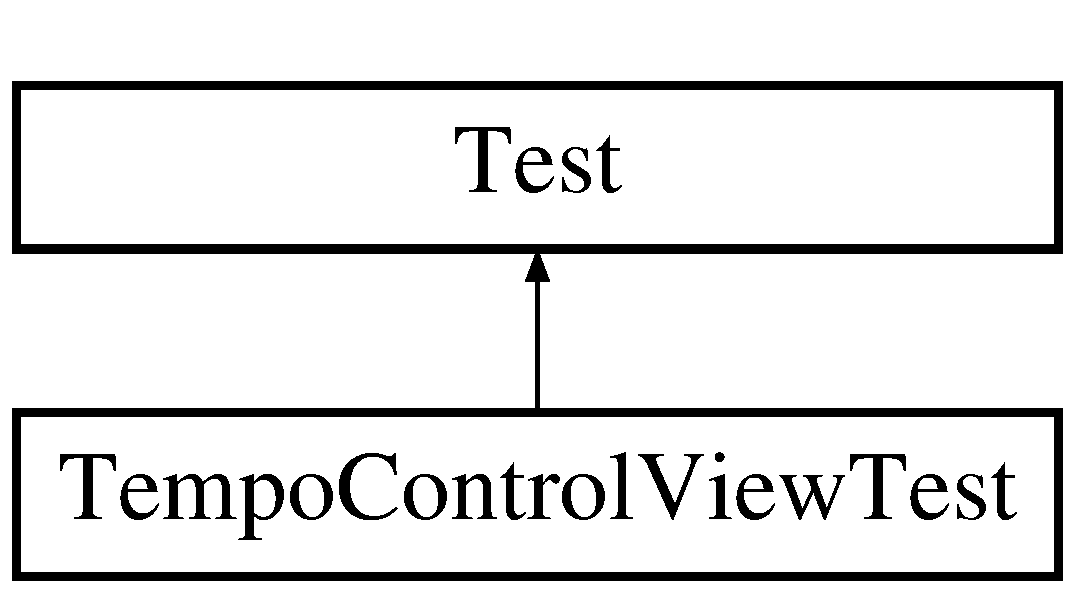
\includegraphics[height=2.000000cm]{class_tempo_control_view_test}
\end{center}
\end{figure}
\subsection*{Public Attributes}
\begin{DoxyCompactItemize}
\item 
\mbox{\Hypertarget{class_tempo_control_view_test_a050771720c01d6c11b704d9ad1cff01f}\label{class_tempo_control_view_test_a050771720c01d6c11b704d9ad1cff01f}} 
Nice\+Mock$<$ \mbox{\hyperlink{class_tempo_timer_mock}{Tempo\+Timer\+Mock}} $>$ {\bfseries timer\+Mock}
\item 
\mbox{\Hypertarget{class_tempo_control_view_test_aecfb3b3851d950e21d396c3e4cee47e7}\label{class_tempo_control_view_test_aecfb3b3851d950e21d396c3e4cee47e7}} 
Nice\+Mock$<$ \mbox{\hyperlink{class_tempo_knob_mock}{Tempo\+Knob\+Mock}} $>$ {\bfseries knob\+Mock}
\item 
\mbox{\Hypertarget{class_tempo_control_view_test_a6af0815cecb1529f78391d9b9cb9dd3d}\label{class_tempo_control_view_test_a6af0815cecb1529f78391d9b9cb9dd3d}} 
Nice\+Mock$<$ \mbox{\hyperlink{class_four_digit_display_mock}{Four\+Digit\+Display\+Mock}} $>$ {\bfseries display\+Mock}
\item 
\mbox{\Hypertarget{class_tempo_control_view_test_aa30375b51fa125e46732b2c16a8c0b6d}\label{class_tempo_control_view_test_aa30375b51fa125e46732b2c16a8c0b6d}} 
\mbox{\hyperlink{class_rhythm_playback_controller}{Rhythm\+Playback\+Controller}} {\bfseries controller} = \mbox{\hyperlink{class_rhythm_playback_controller}{Rhythm\+Playback\+Controller}}(timer\+Mock)
\item 
\mbox{\Hypertarget{class_tempo_control_view_test_abfb369b29db3a42dca9ef54c4a742714}\label{class_tempo_control_view_test_abfb369b29db3a42dca9ef54c4a742714}} 
\mbox{\hyperlink{class_tempo_control_view}{Tempo\+Control\+View}} {\bfseries tempo\+View} = \mbox{\hyperlink{class_tempo_control_view}{Tempo\+Control\+View}}(controller, knob\+Mock, display\+Mock)
\end{DoxyCompactItemize}


The documentation for this class was generated from the following file\+:\begin{DoxyCompactItemize}
\item 
..\textbackslash{}..\textbackslash{}software/presentation/tempo\+\_\+control/tempo\+\_\+control\+\_\+view/test/tempo\+\_\+control\+\_\+view\+\_\+test.\+cpp\end{DoxyCompactItemize}

\hypertarget{class_tempo_knob}{}\section{Tempo\+Knob Class Reference}
\label{class_tempo_knob}\index{TempoKnob@{TempoKnob}}
Inheritance diagram for Tempo\+Knob\+:\begin{figure}[H]
\begin{center}
\leavevmode
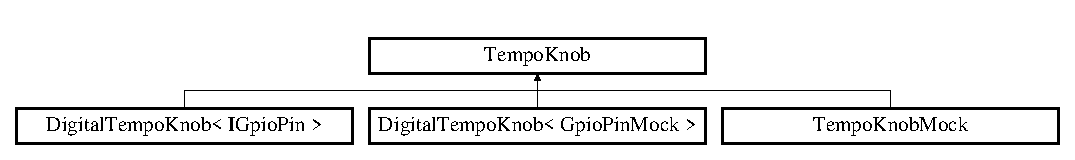
\includegraphics[height=1.696970cm]{class_tempo_knob}
\end{center}
\end{figure}
\subsection*{Public Member Functions}
\begin{DoxyCompactItemize}
\item 
\mbox{\Hypertarget{class_tempo_knob_aac8920db810057a523201b0027d6c852}\label{class_tempo_knob_aac8920db810057a523201b0027d6c852}} 
virtual \mbox{\hyperlink{class_beats_per_minute}{Beats\+Per\+Minute}} {\bfseries read} () const =0
\end{DoxyCompactItemize}


The documentation for this class was generated from the following file\+:\begin{DoxyCompactItemize}
\item 
C\+:/\+Development/code/proj/tr2k\+\_\+drum\+\_\+machine/software/presentation/\+Tempo\+Control/\+Tempo\+Knob/if/Tempo\+Knob.\+h\end{DoxyCompactItemize}

\hypertarget{class_tempo_knob_mock}{}\section{Tempo\+Knob\+Mock Class Reference}
\label{class_tempo_knob_mock}\index{TempoKnobMock@{TempoKnobMock}}
Inheritance diagram for Tempo\+Knob\+Mock\+:\begin{figure}[H]
\begin{center}
\leavevmode
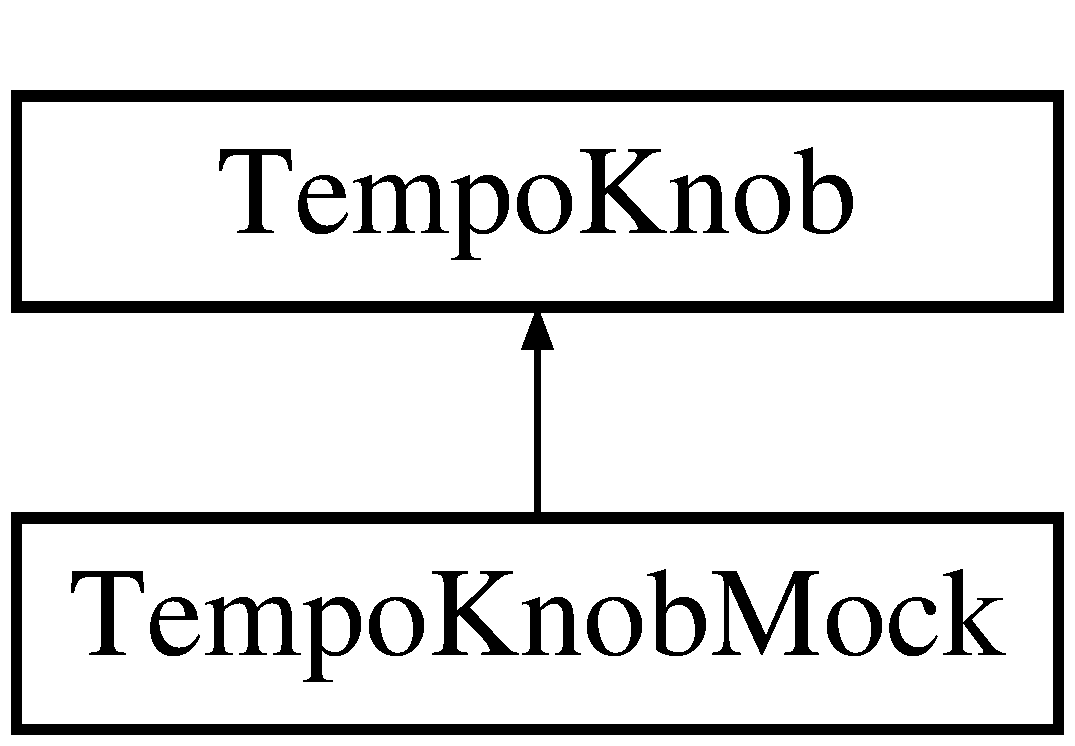
\includegraphics[height=2.000000cm]{class_tempo_knob_mock}
\end{center}
\end{figure}
\subsection*{Public Member Functions}
\begin{DoxyCompactItemize}
\item 
\mbox{\Hypertarget{class_tempo_knob_mock_a2d3e4d224e3972cca38277f9ed25517d}\label{class_tempo_knob_mock_a2d3e4d224e3972cca38277f9ed25517d}} 
{\bfseries M\+O\+C\+K\+\_\+\+C\+O\+N\+S\+T\+\_\+\+M\+E\+T\+H\+O\+D0} (read, \mbox{\hyperlink{class_beats_per_minute}{Beats\+Per\+Minute}}())
\end{DoxyCompactItemize}


The documentation for this class was generated from the following file\+:\begin{DoxyCompactItemize}
\item 
C\+:/\+Development/code/proj/tr2k\+\_\+drum\+\_\+machine/software/presentation/\+Tempo\+Control/\+Tempo\+Knob/if/mock/Tempo\+Knob\+Mock.\+h\end{DoxyCompactItemize}

\hypertarget{class_tempo_timer}{}\section{Tempo\+Timer Class Reference}
\label{class_tempo_timer}\index{Tempo\+Timer@{Tempo\+Timer}}
Inheritance diagram for Tempo\+Timer\+:\begin{figure}[H]
\begin{center}
\leavevmode
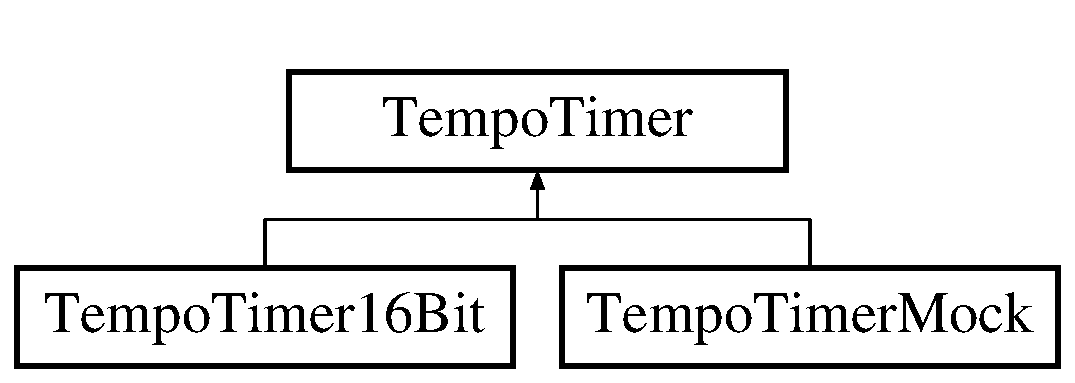
\includegraphics[height=2.000000cm]{class_tempo_timer}
\end{center}
\end{figure}
\subsection*{Public Member Functions}
\begin{DoxyCompactItemize}
\item 
\mbox{\Hypertarget{class_tempo_timer_a7becbb115ca987ae7629f6cb40f6824c}\label{class_tempo_timer_a7becbb115ca987ae7629f6cb40f6824c}} 
virtual void {\bfseries set\+Tempo} (\mbox{\hyperlink{class_beats_per_minute}{Beats\+Per\+Minute}} bpm)=0
\item 
\mbox{\Hypertarget{class_tempo_timer_aa33c53fa2a53e985d833c48a54a6b31c}\label{class_tempo_timer_aa33c53fa2a53e985d833c48a54a6b31c}} 
virtual void {\bfseries start} ()=0
\item 
\mbox{\Hypertarget{class_tempo_timer_addd234d765f7b39bd26da5bc09bf9e0a}\label{class_tempo_timer_addd234d765f7b39bd26da5bc09bf9e0a}} 
virtual void {\bfseries stop} ()=0
\item 
\mbox{\Hypertarget{class_tempo_timer_a2ae88d3a0e961dd42577b8b93e1ab6df}\label{class_tempo_timer_a2ae88d3a0e961dd42577b8b93e1ab6df}} 
virtual void {\bfseries clear} ()=0
\item 
\mbox{\Hypertarget{class_tempo_timer_ac0241c95a4c094bf62aede38cf9de595}\label{class_tempo_timer_ac0241c95a4c094bf62aede38cf9de595}} 
virtual bool {\bfseries playback\+Step\+Is\+Due} ()=0
\item 
\mbox{\Hypertarget{class_tempo_timer_a3758ecc82d1ceaec84076d1852275da3}\label{class_tempo_timer_a3758ecc82d1ceaec84076d1852275da3}} 
virtual void {\bfseries start\+Counting\+Next\+Step} ()=0
\end{DoxyCompactItemize}


The documentation for this class was generated from the following file\+:\begin{DoxyCompactItemize}
\item 
..\textbackslash{}..\textbackslash{}software/domain/rhythm\+\_\+playback/tempo\+\_\+timer/if/tempotimer.\+h\end{DoxyCompactItemize}

\hypertarget{class_tempo_timer16_bit}{}\section{Tempo\+Timer16\+Bit Class Reference}
\label{class_tempo_timer16_bit}\index{Tempo\+Timer16\+Bit@{Tempo\+Timer16\+Bit}}
Inheritance diagram for Tempo\+Timer16\+Bit\+:\begin{figure}[H]
\begin{center}
\leavevmode
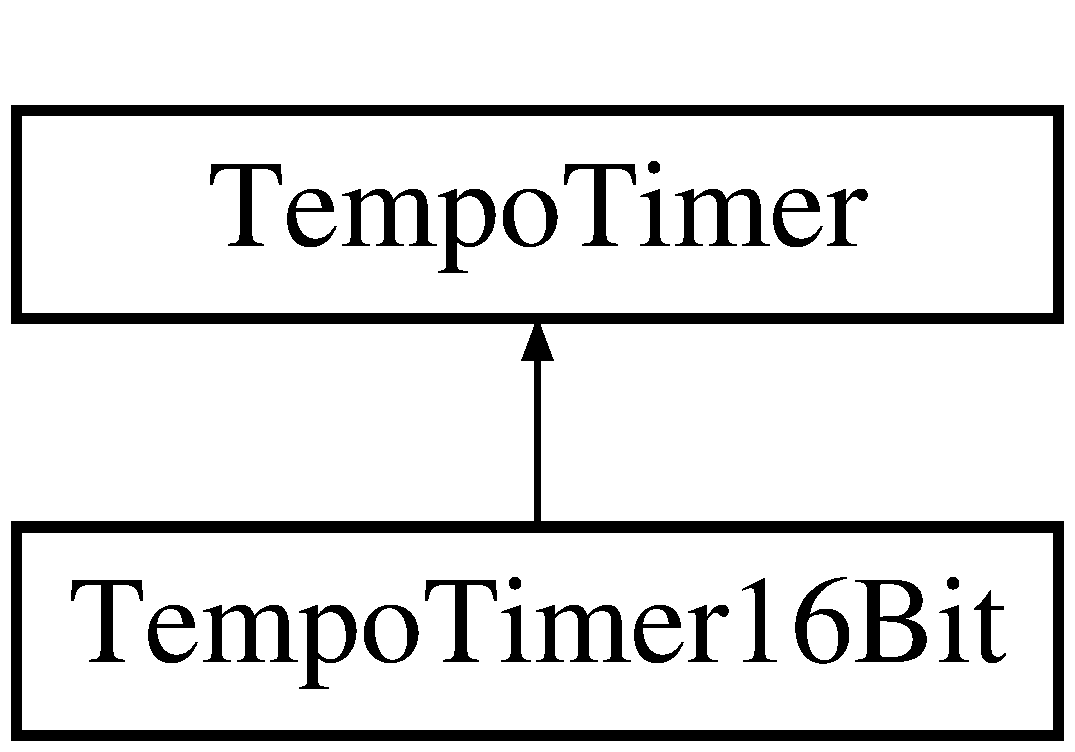
\includegraphics[height=2.000000cm]{class_tempo_timer16_bit}
\end{center}
\end{figure}
\subsection*{Public Member Functions}
\begin{DoxyCompactItemize}
\item 
\mbox{\Hypertarget{class_tempo_timer16_bit_ad1d65ddce9cb60487b7c47f0b4a46dd3}\label{class_tempo_timer16_bit_ad1d65ddce9cb60487b7c47f0b4a46dd3}} 
{\bfseries Tempo\+Timer16\+Bit} (\mbox{\hyperlink{class_timer16_bit}{Timer16\+Bit}} \&timer16\+Bit)
\item 
void \mbox{\hyperlink{class_tempo_timer16_bit_adbd6f0e4af015b240e65109a128988a4}{set\+Tempo}} (\mbox{\hyperlink{class_beats_per_minute}{Beats\+Per\+Minute}} bpm)
\item 
void \mbox{\hyperlink{class_tempo_timer16_bit_a84b46988dda79e20172382417966de13}{start}} ()
\item 
void \mbox{\hyperlink{class_tempo_timer16_bit_abb43b9ec84b965feaf3062aa1cb5be5e}{stop}} ()
\item 
void \mbox{\hyperlink{class_tempo_timer16_bit_a749e01b62ff3ff184c62a99db70588ba}{clear}} ()
\item 
void \mbox{\hyperlink{class_tempo_timer16_bit_a1dcf447b3ffdeadfc65f8bd3da24c632}{count\+Pulse}} ()
\item 
bool \mbox{\hyperlink{class_tempo_timer16_bit_a480d726dc86d7136904056ac4b37082b}{playback\+Step\+Is\+Due}} ()
\item 
void \mbox{\hyperlink{class_tempo_timer16_bit_a1f5d42ac7fe24317a0c04484bbf345c6}{start\+Counting\+Next\+Step}} ()
\end{DoxyCompactItemize}


\subsection{Member Function Documentation}
\mbox{\Hypertarget{class_tempo_timer16_bit_a749e01b62ff3ff184c62a99db70588ba}\label{class_tempo_timer16_bit_a749e01b62ff3ff184c62a99db70588ba}} 
\index{Tempo\+Timer16\+Bit@{Tempo\+Timer16\+Bit}!clear@{clear}}
\index{clear@{clear}!Tempo\+Timer16\+Bit@{Tempo\+Timer16\+Bit}}
\subsubsection{\texorpdfstring{clear()}{clear()}}
{\footnotesize\ttfamily void Tempo\+Timer16\+Bit\+::clear (\begin{DoxyParamCaption}{ }\end{DoxyParamCaption})\hspace{0.3cm}{\ttfamily [virtual]}}

Clears the tempo timer by clearing the underlying 16-\/bit timer. 

Implements \mbox{\hyperlink{class_tempo_timer}{Tempo\+Timer}}.

\mbox{\Hypertarget{class_tempo_timer16_bit_a1dcf447b3ffdeadfc65f8bd3da24c632}\label{class_tempo_timer16_bit_a1dcf447b3ffdeadfc65f8bd3da24c632}} 
\index{Tempo\+Timer16\+Bit@{Tempo\+Timer16\+Bit}!count\+Pulse@{count\+Pulse}}
\index{count\+Pulse@{count\+Pulse}!Tempo\+Timer16\+Bit@{Tempo\+Timer16\+Bit}}
\subsubsection{\texorpdfstring{count\+Pulse()}{countPulse()}}
{\footnotesize\ttfamily void Tempo\+Timer16\+Bit\+::count\+Pulse (\begin{DoxyParamCaption}{ }\end{DoxyParamCaption})}

Count a tempo pulse (pulses-\/per-\/sixteenth-\/note pulses). Used to track when the period for a sixteenth note has elapsed, and the next playback step is due for execution. \mbox{\Hypertarget{class_tempo_timer16_bit_a480d726dc86d7136904056ac4b37082b}\label{class_tempo_timer16_bit_a480d726dc86d7136904056ac4b37082b}} 
\index{Tempo\+Timer16\+Bit@{Tempo\+Timer16\+Bit}!playback\+Step\+Is\+Due@{playback\+Step\+Is\+Due}}
\index{playback\+Step\+Is\+Due@{playback\+Step\+Is\+Due}!Tempo\+Timer16\+Bit@{Tempo\+Timer16\+Bit}}
\subsubsection{\texorpdfstring{playback\+Step\+Is\+Due()}{playbackStepIsDue()}}
{\footnotesize\ttfamily bool Tempo\+Timer16\+Bit\+::playback\+Step\+Is\+Due (\begin{DoxyParamCaption}{ }\end{DoxyParamCaption})\hspace{0.3cm}{\ttfamily [virtual]}}

Should be polled continously by the client. \begin{DoxyReturn}{Returns}
true if the next playback step is due for execution. 
\end{DoxyReturn}


Implements \mbox{\hyperlink{class_tempo_timer}{Tempo\+Timer}}.

\mbox{\Hypertarget{class_tempo_timer16_bit_adbd6f0e4af015b240e65109a128988a4}\label{class_tempo_timer16_bit_adbd6f0e4af015b240e65109a128988a4}} 
\index{Tempo\+Timer16\+Bit@{Tempo\+Timer16\+Bit}!set\+Tempo@{set\+Tempo}}
\index{set\+Tempo@{set\+Tempo}!Tempo\+Timer16\+Bit@{Tempo\+Timer16\+Bit}}
\subsubsection{\texorpdfstring{set\+Tempo()}{setTempo()}}
{\footnotesize\ttfamily void Tempo\+Timer16\+Bit\+::set\+Tempo (\begin{DoxyParamCaption}\item[{\mbox{\hyperlink{class_beats_per_minute}{Beats\+Per\+Minute}}}]{bpm }\end{DoxyParamCaption})\hspace{0.3cm}{\ttfamily [virtual]}}

Sets a tempo in beats per minutes by calculating the corresponding 16-\/bit timer period and assigning it. 

Implements \mbox{\hyperlink{class_tempo_timer}{Tempo\+Timer}}.

\mbox{\Hypertarget{class_tempo_timer16_bit_a84b46988dda79e20172382417966de13}\label{class_tempo_timer16_bit_a84b46988dda79e20172382417966de13}} 
\index{Tempo\+Timer16\+Bit@{Tempo\+Timer16\+Bit}!start@{start}}
\index{start@{start}!Tempo\+Timer16\+Bit@{Tempo\+Timer16\+Bit}}
\subsubsection{\texorpdfstring{start()}{start()}}
{\footnotesize\ttfamily void Tempo\+Timer16\+Bit\+::start (\begin{DoxyParamCaption}{ }\end{DoxyParamCaption})\hspace{0.3cm}{\ttfamily [virtual]}}

Starts the tempo timer by starting the underlying 16-\/bit timer. 

Implements \mbox{\hyperlink{class_tempo_timer}{Tempo\+Timer}}.

\mbox{\Hypertarget{class_tempo_timer16_bit_a1f5d42ac7fe24317a0c04484bbf345c6}\label{class_tempo_timer16_bit_a1f5d42ac7fe24317a0c04484bbf345c6}} 
\index{Tempo\+Timer16\+Bit@{Tempo\+Timer16\+Bit}!start\+Counting\+Next\+Step@{start\+Counting\+Next\+Step}}
\index{start\+Counting\+Next\+Step@{start\+Counting\+Next\+Step}!Tempo\+Timer16\+Bit@{Tempo\+Timer16\+Bit}}
\subsubsection{\texorpdfstring{start\+Counting\+Next\+Step()}{startCountingNextStep()}}
{\footnotesize\ttfamily void Tempo\+Timer16\+Bit\+::start\+Counting\+Next\+Step (\begin{DoxyParamCaption}{ }\end{DoxyParamCaption})\hspace{0.3cm}{\ttfamily [virtual]}}

Used to signal that current playback step has been handled and that the next playback step wait period should start elapsing. Counted pulses are reset. 

Implements \mbox{\hyperlink{class_tempo_timer}{Tempo\+Timer}}.

\mbox{\Hypertarget{class_tempo_timer16_bit_abb43b9ec84b965feaf3062aa1cb5be5e}\label{class_tempo_timer16_bit_abb43b9ec84b965feaf3062aa1cb5be5e}} 
\index{Tempo\+Timer16\+Bit@{Tempo\+Timer16\+Bit}!stop@{stop}}
\index{stop@{stop}!Tempo\+Timer16\+Bit@{Tempo\+Timer16\+Bit}}
\subsubsection{\texorpdfstring{stop()}{stop()}}
{\footnotesize\ttfamily void Tempo\+Timer16\+Bit\+::stop (\begin{DoxyParamCaption}{ }\end{DoxyParamCaption})\hspace{0.3cm}{\ttfamily [virtual]}}

Stops the tempo timer by stopping the underlying 16-\/bit timer. 

Implements \mbox{\hyperlink{class_tempo_timer}{Tempo\+Timer}}.



The documentation for this class was generated from the following files\+:\begin{DoxyCompactItemize}
\item 
..\textbackslash{}..\textbackslash{}software/domain/rhythm\+\_\+playback/tempo\+\_\+timer/inc/tempotimer16bit.\+h\item 
..\textbackslash{}..\textbackslash{}software/domain/rhythm\+\_\+playback/tempo\+\_\+timer/src/tempotimer16bit.\+cpp\end{DoxyCompactItemize}

\hypertarget{class_tempo_timer_mock}{}\section{Tempo\+Timer\+Mock Class Reference}
\label{class_tempo_timer_mock}\index{Tempo\+Timer\+Mock@{Tempo\+Timer\+Mock}}
Inheritance diagram for Tempo\+Timer\+Mock\+:\begin{figure}[H]
\begin{center}
\leavevmode
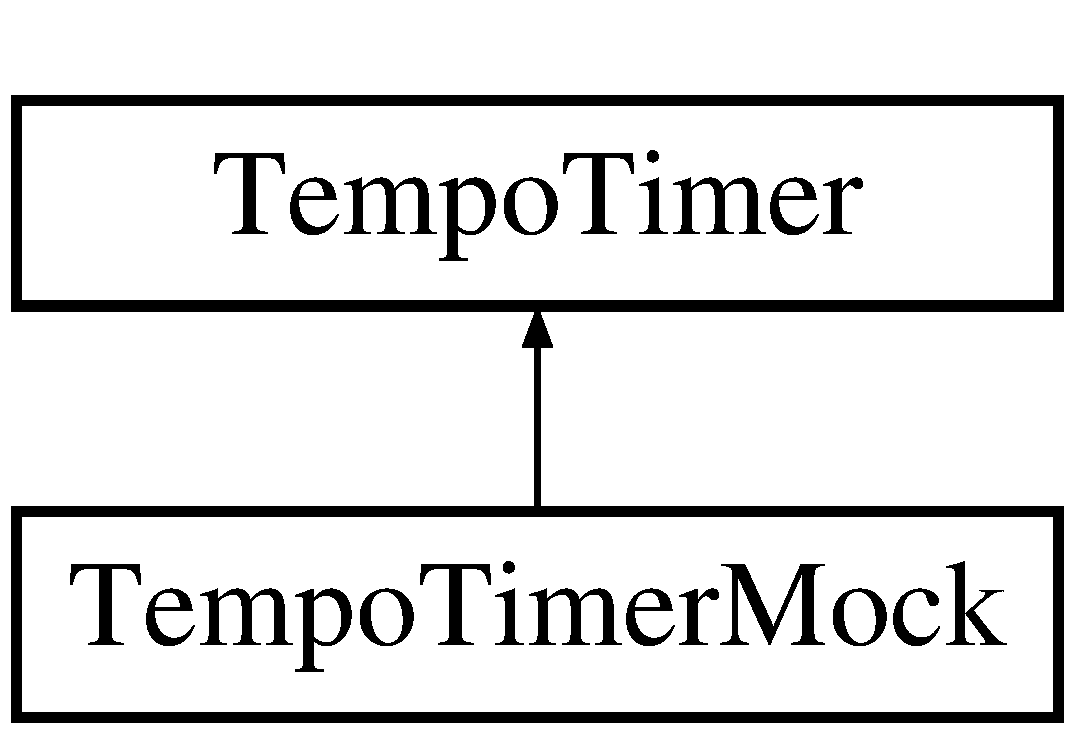
\includegraphics[height=2.000000cm]{class_tempo_timer_mock}
\end{center}
\end{figure}
\subsection*{Public Member Functions}
\begin{DoxyCompactItemize}
\item 
\mbox{\Hypertarget{class_tempo_timer_mock_a744b62ff6f202c876325f757f9ccc836}\label{class_tempo_timer_mock_a744b62ff6f202c876325f757f9ccc836}} 
{\bfseries M\+O\+C\+K\+\_\+\+M\+E\+T\+H\+O\+D1} (set\+Tempo, void(\mbox{\hyperlink{class_beats_per_minute}{Beats\+Per\+Minute}} bpm))
\item 
\mbox{\Hypertarget{class_tempo_timer_mock_a77a9c50cf356c36511139c8270625793}\label{class_tempo_timer_mock_a77a9c50cf356c36511139c8270625793}} 
{\bfseries M\+O\+C\+K\+\_\+\+M\+E\+T\+H\+O\+D0} (start, void())
\item 
\mbox{\Hypertarget{class_tempo_timer_mock_a79ac2d1e81fe29d3301b8c38c93879d1}\label{class_tempo_timer_mock_a79ac2d1e81fe29d3301b8c38c93879d1}} 
{\bfseries M\+O\+C\+K\+\_\+\+M\+E\+T\+H\+O\+D0} (stop, void())
\item 
\mbox{\Hypertarget{class_tempo_timer_mock_a2a9634cefd6bafe16cd7f09621a57fe9}\label{class_tempo_timer_mock_a2a9634cefd6bafe16cd7f09621a57fe9}} 
{\bfseries M\+O\+C\+K\+\_\+\+M\+E\+T\+H\+O\+D0} (clear, void())
\item 
\mbox{\Hypertarget{class_tempo_timer_mock_ac38619037ba0cdc4659286cb512ff08a}\label{class_tempo_timer_mock_ac38619037ba0cdc4659286cb512ff08a}} 
{\bfseries M\+O\+C\+K\+\_\+\+M\+E\+T\+H\+O\+D0} (playback\+Step\+Is\+Due, bool())
\item 
\mbox{\Hypertarget{class_tempo_timer_mock_a2db4e5a24a1e9e2c253d9efcc8a3f6c5}\label{class_tempo_timer_mock_a2db4e5a24a1e9e2c253d9efcc8a3f6c5}} 
{\bfseries M\+O\+C\+K\+\_\+\+M\+E\+T\+H\+O\+D0} (start\+Counting\+Next\+Step, void())
\end{DoxyCompactItemize}


The documentation for this class was generated from the following file\+:\begin{DoxyCompactItemize}
\item 
..\textbackslash{}..\textbackslash{}software/domain/rhythm\+\_\+playback/tempo\+\_\+timer/if/mock/tempotimermock.\+h\end{DoxyCompactItemize}

\hypertarget{class_tempo_timing_manager}{}\section{Tempo\+Timing\+Manager Class Reference}
\label{class_tempo_timing_manager}\index{Tempo\+Timing\+Manager@{Tempo\+Timing\+Manager}}
\subsection*{Public Member Functions}
\begin{DoxyCompactItemize}
\item 
\mbox{\Hypertarget{class_tempo_timing_manager_a1001a3fdd1d051076fb440da068cf11a}\label{class_tempo_timing_manager_a1001a3fdd1d051076fb440da068cf11a}} 
{\bfseries Tempo\+Timing\+Manager} (\mbox{\hyperlink{class_tempo_timer}{Tempo\+Timer}} \&tempo\+Timer)
\item 
void \mbox{\hyperlink{class_tempo_timing_manager_aff742971bd50205edc863163c7674740}{add\+Playback\+Step\+Handler}} (Playback\+Step\+Handler handler)
\item 
void \mbox{\hyperlink{class_tempo_timing_manager_a697545e7fa499a13630d2f224eac4fac}{handle\+Playback}} ()
\end{DoxyCompactItemize}
\subsection*{Static Public Attributes}
\begin{DoxyCompactItemize}
\item 
\mbox{\Hypertarget{class_tempo_timing_manager_aa0987abea44aeac79ca46b859ae444a1}\label{class_tempo_timing_manager_aa0987abea44aeac79ca46b859ae444a1}} 
static constexpr u8 {\bfseries max\+Num\+Handlers} = 16
\end{DoxyCompactItemize}


\subsection{Member Function Documentation}
\mbox{\Hypertarget{class_tempo_timing_manager_aff742971bd50205edc863163c7674740}\label{class_tempo_timing_manager_aff742971bd50205edc863163c7674740}} 
\index{Tempo\+Timing\+Manager@{Tempo\+Timing\+Manager}!add\+Playback\+Step\+Handler@{add\+Playback\+Step\+Handler}}
\index{add\+Playback\+Step\+Handler@{add\+Playback\+Step\+Handler}!Tempo\+Timing\+Manager@{Tempo\+Timing\+Manager}}
\subsubsection{\texorpdfstring{add\+Playback\+Step\+Handler()}{addPlaybackStepHandler()}}
{\footnotesize\ttfamily void Tempo\+Timing\+Manager\+::add\+Playback\+Step\+Handler (\begin{DoxyParamCaption}\item[{Playback\+Step\+Handler}]{handler }\end{DoxyParamCaption})}

Add a new callback to be called in the \mbox{\hyperlink{class_tempo_timing_manager_a697545e7fa499a13630d2f224eac4fac}{handle\+Playback()}} method. If maximum number of callbacks registered, this method does nothing. \mbox{\Hypertarget{class_tempo_timing_manager_a697545e7fa499a13630d2f224eac4fac}\label{class_tempo_timing_manager_a697545e7fa499a13630d2f224eac4fac}} 
\index{Tempo\+Timing\+Manager@{Tempo\+Timing\+Manager}!handle\+Playback@{handle\+Playback}}
\index{handle\+Playback@{handle\+Playback}!Tempo\+Timing\+Manager@{Tempo\+Timing\+Manager}}
\subsubsection{\texorpdfstring{handle\+Playback()}{handlePlayback()}}
{\footnotesize\ttfamily void Tempo\+Timing\+Manager\+::handle\+Playback (\begin{DoxyParamCaption}{ }\end{DoxyParamCaption})}

Checks with the \mbox{\hyperlink{class_tempo_timer}{Tempo\+Timer}} if a playback step is due for execution. If it is, all registered playback step handler callbacks are called. 

The documentation for this class was generated from the following files\+:\begin{DoxyCompactItemize}
\item 
..\textbackslash{}..\textbackslash{}software/domain/rhythm\+\_\+playback/tempo\+\_\+timing\+\_\+manager/inc/tempotimingmanager.\+h\item 
..\textbackslash{}..\textbackslash{}software/domain/rhythm\+\_\+playback/tempo\+\_\+timing\+\_\+manager/src/tempotimingmanager.\+cpp\end{DoxyCompactItemize}

\hypertarget{class_test_beats_per_minute}{}\section{Test\+Beats\+Per\+Minute Class Reference}
\label{class_test_beats_per_minute}\index{Test\+Beats\+Per\+Minute@{Test\+Beats\+Per\+Minute}}
Inheritance diagram for Test\+Beats\+Per\+Minute\+:\begin{figure}[H]
\begin{center}
\leavevmode
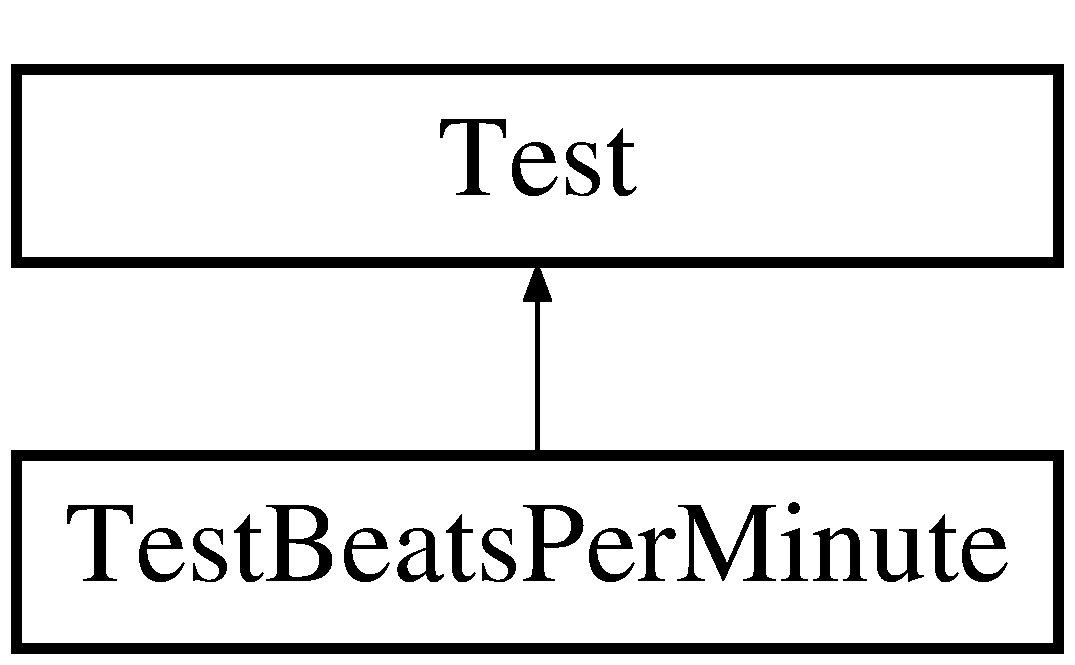
\includegraphics[height=2.000000cm]{class_test_beats_per_minute}
\end{center}
\end{figure}


The documentation for this class was generated from the following file\+:\begin{DoxyCompactItemize}
\item 
..\textbackslash{}..\textbackslash{}software/domain/rhythm\+\_\+playback/beats\+\_\+per\+\_\+minute/test/beatsperminute\+\_\+test.\+cpp\end{DoxyCompactItemize}

\hypertarget{class_test_gpio_pin}{}\section{Test\+Gpio\+Pin Class Reference}
\label{class_test_gpio_pin}\index{TestGpioPin@{TestGpioPin}}
Inheritance diagram for Test\+Gpio\+Pin\+:\begin{figure}[H]
\begin{center}
\leavevmode
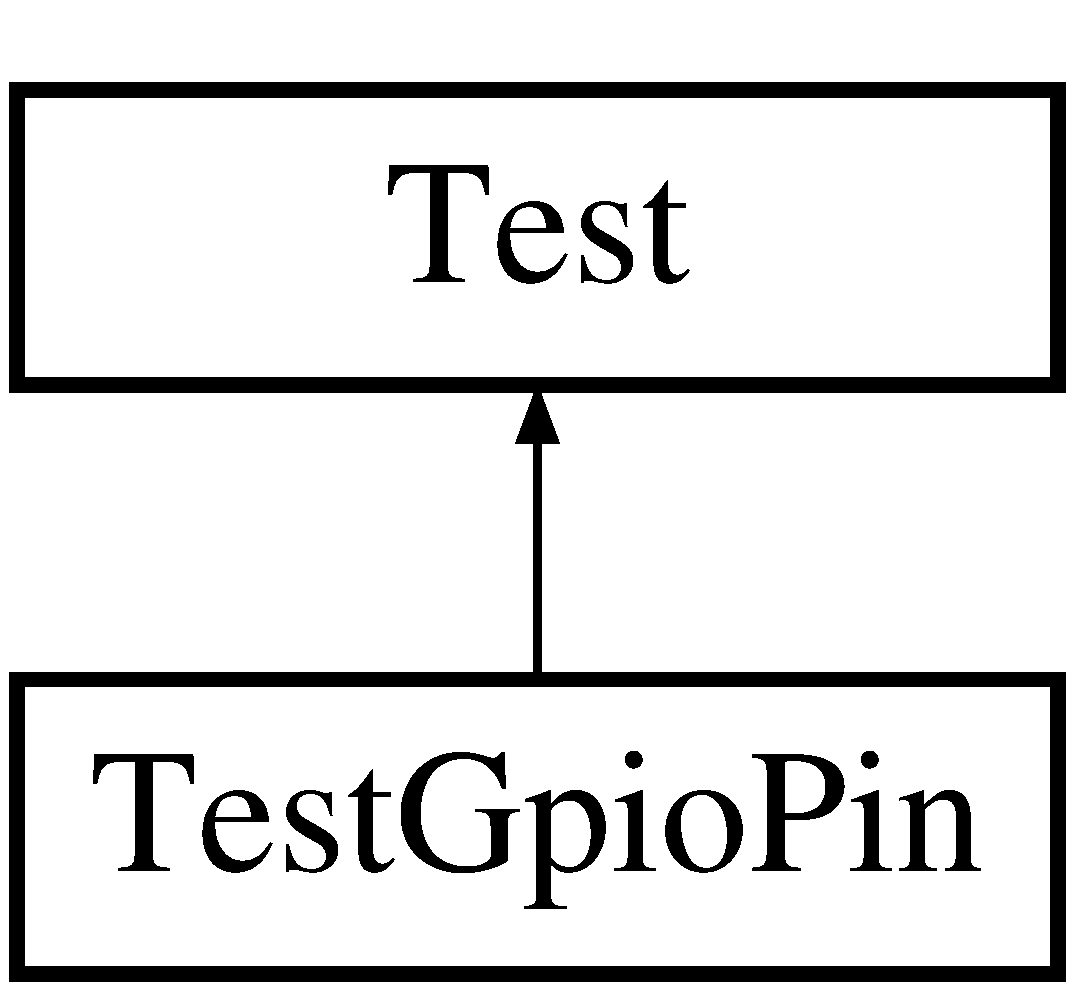
\includegraphics[height=2.000000cm]{class_test_gpio_pin}
\end{center}
\end{figure}
\subsection*{Public Member Functions}
\begin{DoxyCompactItemize}
\item 
\mbox{\Hypertarget{class_test_gpio_pin_a16dac6c5fc1a9d2a192e9ece77e68e08}\label{class_test_gpio_pin_a16dac6c5fc1a9d2a192e9ece77e68e08}} 
void {\bfseries Set\+Up} ()
\end{DoxyCompactItemize}
\subsection*{Public Attributes}
\begin{DoxyCompactItemize}
\item 
\mbox{\Hypertarget{class_test_gpio_pin_abfdc244ab65eef13ffe89867e360dcb1}\label{class_test_gpio_pin_abfdc244ab65eef13ffe89867e360dcb1}} 
\mbox{\hyperlink{class_gpio_pin}{Gpio\+Pin}} {\bfseries test\+Pin} = \mbox{\hyperlink{class_gpio_pin}{Gpio\+Pin}}(Pin0, PortB)
\item 
std\+::vector$<$ \mbox{\hyperlink{class_gpio_pin}{Gpio\+Pin}} $>$ {\bfseries test\+Pins}
\item 
\mbox{\Hypertarget{class_test_gpio_pin_a8624b302e310f70ff1d836765ac70d42}\label{class_test_gpio_pin_a8624b302e310f70ff1d836765ac70d42}} 
uint8\+\_\+t {\bfseries input\+Register} = 0
\item 
\mbox{\Hypertarget{class_test_gpio_pin_a14d28ad10e22bc6ad548e967a7ba8cdf}\label{class_test_gpio_pin_a14d28ad10e22bc6ad548e967a7ba8cdf}} 
uint8\+\_\+t {\bfseries output\+Register} = 0
\item 
\mbox{\Hypertarget{class_test_gpio_pin_ac17d157baca46eaede873ce26bd766fc}\label{class_test_gpio_pin_ac17d157baca46eaede873ce26bd766fc}} 
uint8\+\_\+t {\bfseries data\+Direction\+Register} = 0
\end{DoxyCompactItemize}


\subsection{Member Data Documentation}
\mbox{\Hypertarget{class_test_gpio_pin_a9f11ed851f5dc2f0a9d73a8176c58560}\label{class_test_gpio_pin_a9f11ed851f5dc2f0a9d73a8176c58560}} 
\index{TestGpioPin@{TestGpioPin}!testPins@{testPins}}
\index{testPins@{testPins}!TestGpioPin@{TestGpioPin}}
\subsubsection{\texorpdfstring{testPins}{testPins}}
{\footnotesize\ttfamily std\+::vector$<$\mbox{\hyperlink{class_gpio_pin}{Gpio\+Pin}}$>$ Test\+Gpio\+Pin\+::test\+Pins}

{\bfseries Initial value\+:}
\begin{DoxyCode}{0}
\DoxyCodeLine{= \{ \mbox{\hyperlink{class_gpio_pin}{GpioPin}}(Pin0, PortB),}
\DoxyCodeLine{        \mbox{\hyperlink{class_gpio_pin}{GpioPin}}(Pin1, PortB), \mbox{\hyperlink{class_gpio_pin}{GpioPin}}(Pin2, PortB) \}}

\end{DoxyCode}


The documentation for this class was generated from the following file\+:\begin{DoxyCompactItemize}
\item 
C\+:/\+Development/code/proj/tr2k\+\_\+drum\+\_\+machine/software/drivers/\+Gpio\+Pin/test/Gpio\+Pin\+Test.\+cpp\end{DoxyCompactItemize}

\hypertarget{class_test_interrupts}{}\section{Test\+Interrupts Class Reference}
\label{class_test_interrupts}\index{Test\+Interrupts@{Test\+Interrupts}}
Inheritance diagram for Test\+Interrupts\+:\begin{figure}[H]
\begin{center}
\leavevmode
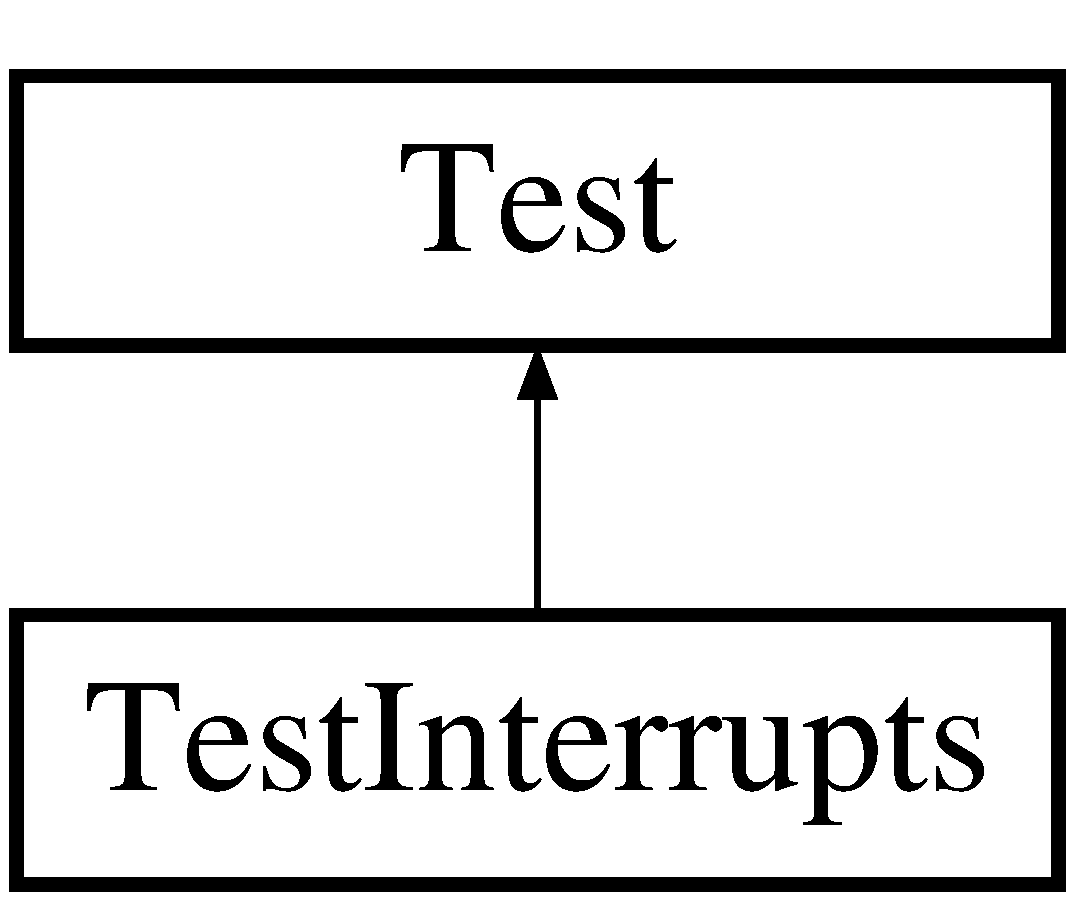
\includegraphics[height=2.000000cm]{class_test_interrupts}
\end{center}
\end{figure}
\subsection*{Public Member Functions}
\begin{DoxyCompactItemize}
\item 
\mbox{\Hypertarget{class_test_interrupts_a21921f75ea496b1bfdc5e4ed6d335db8}\label{class_test_interrupts_a21921f75ea496b1bfdc5e4ed6d335db8}} 
void {\bfseries Set\+Up} ()
\item 
void \mbox{\hyperlink{class_test_interrupts_ab6080c1aab065f65cf6c7c6e4fd271a0}{test\+Interrupt\+Handler\+Calls\+Callback}} (Interrupt\+Handler interrupt\+Handler, Interrupt\+Request interrupt\+Request, Interrupt\+Service\+Routine service\+Routine, std\+::string interrupt\+Name)
\end{DoxyCompactItemize}


\subsection{Member Function Documentation}
\mbox{\Hypertarget{class_test_interrupts_ab6080c1aab065f65cf6c7c6e4fd271a0}\label{class_test_interrupts_ab6080c1aab065f65cf6c7c6e4fd271a0}} 
\index{Test\+Interrupts@{Test\+Interrupts}!test\+Interrupt\+Handler\+Calls\+Callback@{test\+Interrupt\+Handler\+Calls\+Callback}}
\index{test\+Interrupt\+Handler\+Calls\+Callback@{test\+Interrupt\+Handler\+Calls\+Callback}!Test\+Interrupts@{Test\+Interrupts}}
\subsubsection{\texorpdfstring{test\+Interrupt\+Handler\+Calls\+Callback()}{testInterruptHandlerCallsCallback()}}
{\footnotesize\ttfamily void Test\+Interrupts\+::test\+Interrupt\+Handler\+Calls\+Callback (\begin{DoxyParamCaption}\item[{Interrupt\+Handler}]{interrupt\+Handler,  }\item[{Interrupt\+Request}]{interrupt\+Request,  }\item[{Interrupt\+Service\+Routine}]{service\+Routine,  }\item[{std\+::string}]{interrupt\+Name }\end{DoxyParamCaption})\hspace{0.3cm}{\ttfamily [inline]}}

Helper function for testing that handlers attached to an interrupt gets called from the corresponding service routine (which is the destination from the interrupt vector). 
\begin{DoxyParams}{Parameters}
{\em interrupt\+Handler} & pointer to function to be called from service routine \\
\hline
{\em interrupt\+Request} & enum specifying interrupt signal to attach handler to \\
\hline
{\em service\+Routine} & pointer to interrupt service routine belonging to interrupt \\
\hline
{\em interrupt\+Name} & name of interrupt to print out in assertion error message \\
\hline
\end{DoxyParams}


The documentation for this class was generated from the following file\+:\begin{DoxyCompactItemize}
\item 
..\textbackslash{}..\textbackslash{}software/infrastructure/interrupts/test/interrupt\+\_\+test.\+cpp\end{DoxyCompactItemize}

\hypertarget{class_test_rhythm_playback_controller}{}\section{Test\+Rhythm\+Playback\+Controller Class Reference}
\label{class_test_rhythm_playback_controller}\index{Test\+Rhythm\+Playback\+Controller@{Test\+Rhythm\+Playback\+Controller}}
Inheritance diagram for Test\+Rhythm\+Playback\+Controller\+:\begin{figure}[H]
\begin{center}
\leavevmode
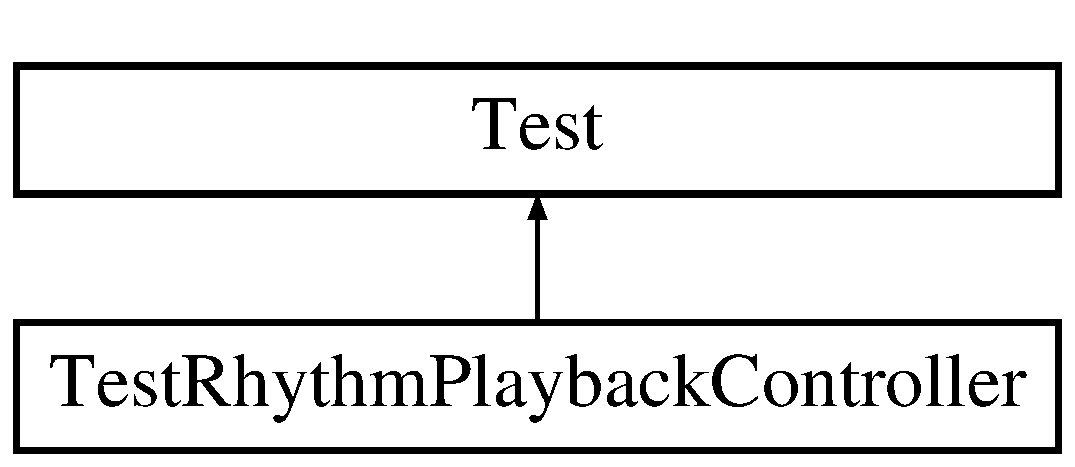
\includegraphics[height=2.000000cm]{class_test_rhythm_playback_controller}
\end{center}
\end{figure}
\subsection*{Public Attributes}
\begin{DoxyCompactItemize}
\item 
\mbox{\Hypertarget{class_test_rhythm_playback_controller_abe8f6c5c945fc43aa1c4feb96ba30f64}\label{class_test_rhythm_playback_controller_abe8f6c5c945fc43aa1c4feb96ba30f64}} 
\mbox{\hyperlink{class_tempo_timer_mock}{Tempo\+Timer\+Mock}} {\bfseries timer\+Mock}
\item 
\mbox{\Hypertarget{class_test_rhythm_playback_controller_a2dbfa579ee33a84cead39a167cdc28e2}\label{class_test_rhythm_playback_controller_a2dbfa579ee33a84cead39a167cdc28e2}} 
\mbox{\hyperlink{class_rhythm_playback_controller}{Rhythm\+Playback\+Controller}} {\bfseries controller} = \mbox{\hyperlink{class_rhythm_playback_controller}{Rhythm\+Playback\+Controller}}(timer\+Mock)
\end{DoxyCompactItemize}


The documentation for this class was generated from the following file\+:\begin{DoxyCompactItemize}
\item 
..\textbackslash{}..\textbackslash{}software/application/rhythm\+\_\+playback\+\_\+controller/test/rhythm\+\_\+playback\+\_\+controller\+\_\+test.\+cpp\end{DoxyCompactItemize}

\hypertarget{class_test_segment_display74_h_c595}{}\section{Test\+Segment\+Display74\+H\+C595 Class Reference}
\label{class_test_segment_display74_h_c595}\index{TestSegmentDisplay74HC595@{TestSegmentDisplay74HC595}}
Inheritance diagram for Test\+Segment\+Display74\+H\+C595\+:\begin{figure}[H]
\begin{center}
\leavevmode
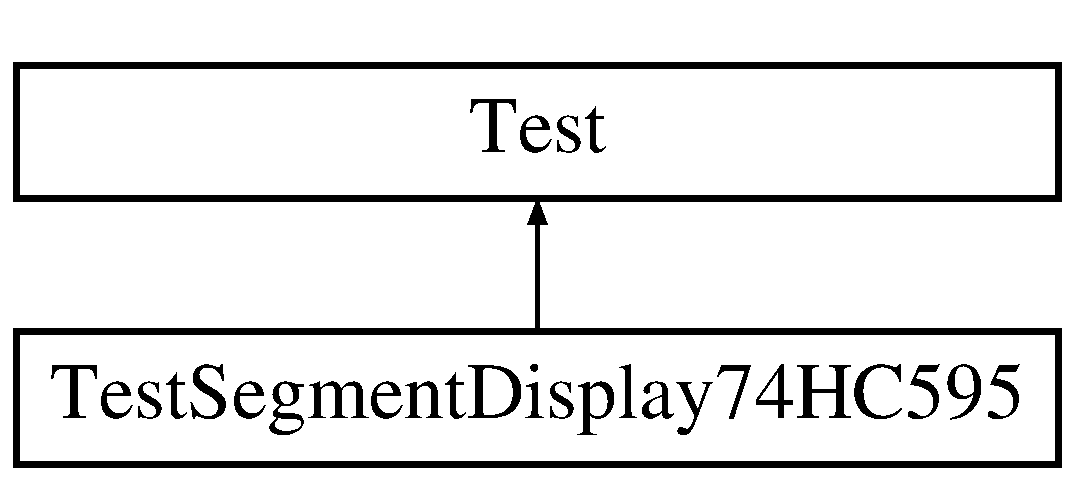
\includegraphics[height=2.000000cm]{class_test_segment_display74_h_c595}
\end{center}
\end{figure}
\subsection*{Public Attributes}
\begin{DoxyCompactItemize}
\item 
\mbox{\Hypertarget{class_test_segment_display74_h_c595_af2798ef4f77230c853c944bc049a6082}\label{class_test_segment_display74_h_c595_af2798ef4f77230c853c944bc049a6082}} 
u8 {\bfseries pin\+Direction\+Reg} = 0
\item 
\mbox{\Hypertarget{class_test_segment_display74_h_c595_aa81517db050dcb1bfc54c5ccce0de0fa}\label{class_test_segment_display74_h_c595_aa81517db050dcb1bfc54c5ccce0de0fa}} 
u8 {\bfseries control\+Reg} = 0
\item 
\mbox{\Hypertarget{class_test_segment_display74_h_c595_a59e27e6533a5dade8460c3acd1c2a4bc}\label{class_test_segment_display74_h_c595_a59e27e6533a5dade8460c3acd1c2a4bc}} 
u8 {\bfseries status\+Reg} = 0
\item 
\mbox{\Hypertarget{class_test_segment_display74_h_c595_a343a03e0831f6efcdeb675dceb1949ff}\label{class_test_segment_display74_h_c595_a343a03e0831f6efcdeb675dceb1949ff}} 
u8 {\bfseries data\+Reg} = 0
\item 
\mbox{\Hypertarget{class_test_segment_display74_h_c595_ab093597d558c95849a23fce5886fadea}\label{class_test_segment_display74_h_c595_ab093597d558c95849a23fce5886fadea}} 
\mbox{\hyperlink{class_spi}{Spi}} {\bfseries spi} = \mbox{\hyperlink{class_spi}{Spi}}(pin\+Direction\+Reg, control\+Reg, status\+Reg, data\+Reg)
\item 
\mbox{\Hypertarget{class_test_segment_display74_h_c595_aaa666829ff3f82cf4d8ec37a97cdf13b}\label{class_test_segment_display74_h_c595_aaa666829ff3f82cf4d8ec37a97cdf13b}} 
\mbox{\hyperlink{class_segment_display74_h_c595}{Segment\+Display74\+H\+C595}} {\bfseries display} = \mbox{\hyperlink{class_segment_display74_h_c595}{Segment\+Display74\+H\+C595}}(spi)
\item 
std\+::map$<$ digit\+Value, segment\+Data $>$ {\bfseries segment\+Data\+Look\+Up\+Table}
\end{DoxyCompactItemize}


\subsection{Member Data Documentation}
\mbox{\Hypertarget{class_test_segment_display74_h_c595_a5adfa8af8f14cedfff1ae6129d423355}\label{class_test_segment_display74_h_c595_a5adfa8af8f14cedfff1ae6129d423355}} 
\index{TestSegmentDisplay74HC595@{TestSegmentDisplay74HC595}!segmentDataLookUpTable@{segmentDataLookUpTable}}
\index{segmentDataLookUpTable@{segmentDataLookUpTable}!TestSegmentDisplay74HC595@{TestSegmentDisplay74HC595}}
\subsubsection{\texorpdfstring{segmentDataLookUpTable}{segmentDataLookUpTable}}
{\footnotesize\ttfamily std\+::map$<$digit\+Value, segment\+Data$>$ Test\+Segment\+Display74\+H\+C595\+::segment\+Data\+Look\+Up\+Table}

{\bfseries Initial value\+:}
\begin{DoxyCode}{0}
\DoxyCodeLine{=}
\DoxyCodeLine{    \{}
\DoxyCodeLine{        \{0, 0xC0\}, \{1, 0xF9\}, \{2, 0xA4\}, \{3, 0xB0\}, \{4, 0x99\},}
\DoxyCodeLine{        \{5, 0x92\}, \{6, 0x82\}, \{7, 0xF8\}, \{8, 0x80\}, \{9, 0x90\}}
\DoxyCodeLine{    \}}

\end{DoxyCode}


The documentation for this class was generated from the following file\+:\begin{DoxyCompactItemize}
\item 
C\+:/\+Development/code/proj/tr2k\+\_\+drum\+\_\+machine/software/drivers/\+Segment\+Display/test/Segment\+Display\+Test.\+cpp\end{DoxyCompactItemize}

\hypertarget{class_test_tempo_timer16_bit}{}\section{Test\+Tempo\+Timer16\+Bit Class Reference}
\label{class_test_tempo_timer16_bit}\index{TestTempoTimer16Bit@{TestTempoTimer16Bit}}
Inheritance diagram for Test\+Tempo\+Timer16\+Bit\+:\begin{figure}[H]
\begin{center}
\leavevmode
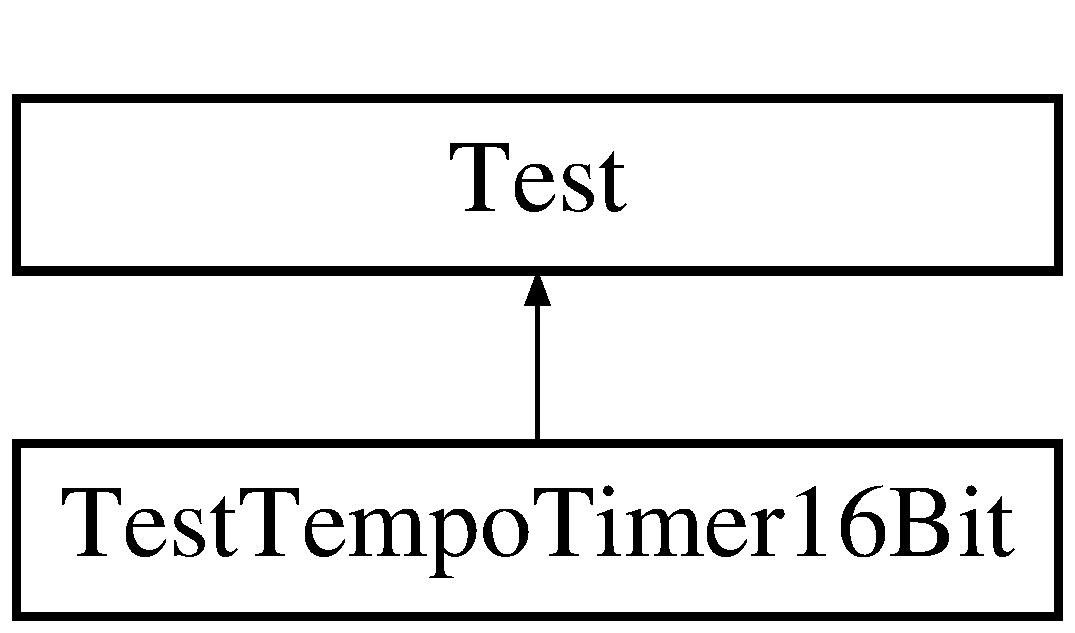
\includegraphics[height=2.000000cm]{class_test_tempo_timer16_bit}
\end{center}
\end{figure}
\subsection*{Public Member Functions}
\begin{DoxyCompactItemize}
\item 
\mbox{\Hypertarget{class_test_tempo_timer16_bit_a0686c53579db8bafbc86afb8159254de}\label{class_test_tempo_timer16_bit_a0686c53579db8bafbc86afb8159254de}} 
void {\bfseries count\+Tempo\+Pulses} (u16 num\+Pulses)
\end{DoxyCompactItemize}
\subsection*{Public Attributes}
\begin{DoxyCompactItemize}
\item 
\mbox{\Hypertarget{class_test_tempo_timer16_bit_aa260c814720ac243dae4f16949730bea}\label{class_test_tempo_timer16_bit_aa260c814720ac243dae4f16949730bea}} 
Nice\+Mock$<$ \mbox{\hyperlink{class_timer16_bit_mock}{Timer16\+Bit\+Mock}} $>$ {\bfseries timer16\+Mock}
\item 
\mbox{\Hypertarget{class_test_tempo_timer16_bit_ab636f3982d6a96505efd66385f111814}\label{class_test_tempo_timer16_bit_ab636f3982d6a96505efd66385f111814}} 
\mbox{\hyperlink{class_tempo_timer16_bit}{Tempo\+Timer16\+Bit}} {\bfseries tempo\+Timer} = \mbox{\hyperlink{class_tempo_timer16_bit}{Tempo\+Timer16\+Bit}}(timer16\+Mock)
\end{DoxyCompactItemize}


The documentation for this class was generated from the following file\+:\begin{DoxyCompactItemize}
\item 
C\+:/\+Development/code/proj/tr2k\+\_\+drum\+\_\+machine/software/domain/\+Rhythm\+Playback/\+Tempo\+Timer/test/Tempo\+Timer16\+Bit\+Test.\+cpp\end{DoxyCompactItemize}

\hypertarget{class_test_tempo_timing_manager}{}\section{Test\+Tempo\+Timing\+Manager Class Reference}
\label{class_test_tempo_timing_manager}\index{Test\+Tempo\+Timing\+Manager@{Test\+Tempo\+Timing\+Manager}}
Inheritance diagram for Test\+Tempo\+Timing\+Manager\+:\begin{figure}[H]
\begin{center}
\leavevmode
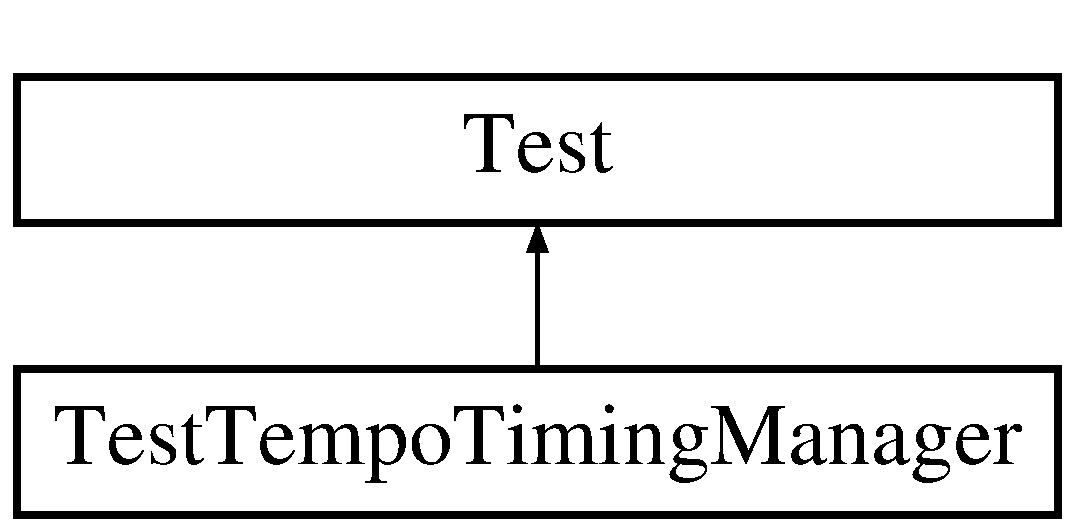
\includegraphics[height=2.000000cm]{class_test_tempo_timing_manager}
\end{center}
\end{figure}
\subsection*{Public Member Functions}
\begin{DoxyCompactItemize}
\item 
\mbox{\Hypertarget{class_test_tempo_timing_manager_ab2dd23b7793242f68e6d4b577f2d46ee}\label{class_test_tempo_timing_manager_ab2dd23b7793242f68e6d4b577f2d46ee}} 
void {\bfseries Set\+Up} ()
\end{DoxyCompactItemize}
\subsection*{Public Attributes}
\begin{DoxyCompactItemize}
\item 
\mbox{\Hypertarget{class_test_tempo_timing_manager_a9b82197ab9c924bfbcc294e0f8a3d115}\label{class_test_tempo_timing_manager_a9b82197ab9c924bfbcc294e0f8a3d115}} 
Nice\+Mock$<$ \mbox{\hyperlink{class_tempo_timer_mock}{Tempo\+Timer\+Mock}} $>$ {\bfseries mock\+Timer}
\item 
\mbox{\Hypertarget{class_test_tempo_timing_manager_a270baf608cf066d37fafaf89dd79c8d1}\label{class_test_tempo_timing_manager_a270baf608cf066d37fafaf89dd79c8d1}} 
\mbox{\hyperlink{class_tempo_timing_manager}{Tempo\+Timing\+Manager}} {\bfseries timing\+Manager} = \mbox{\hyperlink{class_tempo_timing_manager}{Tempo\+Timing\+Manager}}(mock\+Timer)
\end{DoxyCompactItemize}


The documentation for this class was generated from the following file\+:\begin{DoxyCompactItemize}
\item 
..\textbackslash{}..\textbackslash{}software/domain/rhythm\+\_\+playback/tempo\+\_\+timing\+\_\+manager/test/tempotimingmanager\+\_\+test.\+cpp\end{DoxyCompactItemize}

\hypertarget{class_test_timer0}{}\section{Test\+Timer0 Class Reference}
\label{class_test_timer0}\index{Test\+Timer0@{Test\+Timer0}}
Inheritance diagram for Test\+Timer0\+:\begin{figure}[H]
\begin{center}
\leavevmode
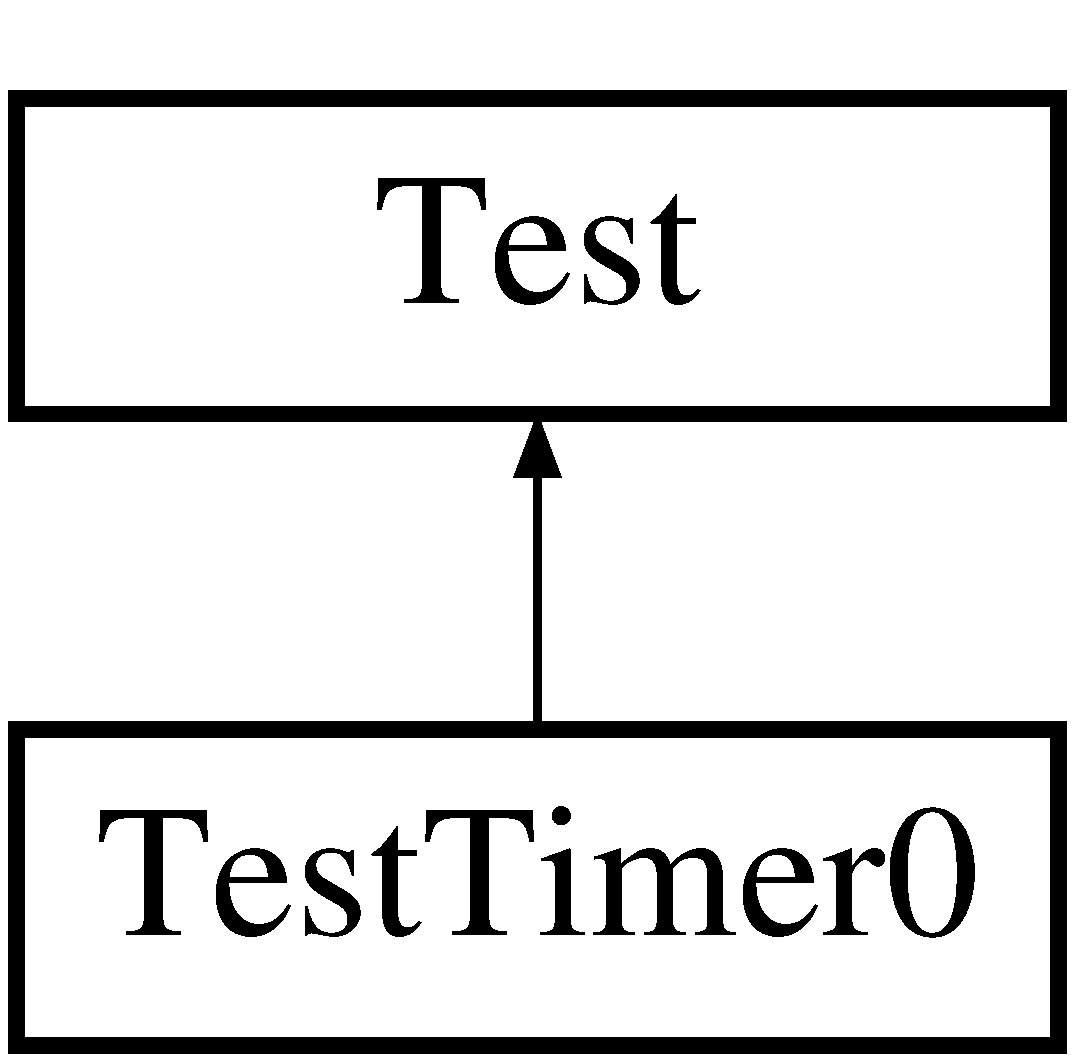
\includegraphics[height=2.000000cm]{class_test_timer0}
\end{center}
\end{figure}
\subsection*{Public Member Functions}
\begin{DoxyCompactItemize}
\item 
\mbox{\Hypertarget{class_test_timer0_abb854fcebd77c9d93b5154f6ada10ebb}\label{class_test_timer0_abb854fcebd77c9d93b5154f6ada10ebb}} 
void {\bfseries Set\+Up} ()
\item 
\mbox{\Hypertarget{class_test_timer0_a9d9b41cb2775201328c8123cb9d26950}\label{class_test_timer0_a9d9b41cb2775201328c8123cb9d26950}} 
void {\bfseries test\+Prescaler} (Timer8\+Bit\+::\+Prescale\+Option prescaler, u8 clock\+Select\+Bits)
\end{DoxyCompactItemize}
\subsection*{Public Attributes}
\begin{DoxyCompactItemize}
\item 
\mbox{\Hypertarget{class_test_timer0_aa22a6242e48d5315ea17a1a001c819dd}\label{class_test_timer0_aa22a6242e48d5315ea17a1a001c819dd}} 
u8 {\bfseries control\+RegisterA} = 0
\item 
\mbox{\Hypertarget{class_test_timer0_a2d800f86dd254e32cab71fb5595d4391}\label{class_test_timer0_a2d800f86dd254e32cab71fb5595d4391}} 
u8 {\bfseries control\+RegisterB} = 0
\item 
\mbox{\Hypertarget{class_test_timer0_a23a7a97c609bb8a7ea3307266481e26b}\label{class_test_timer0_a23a7a97c609bb8a7ea3307266481e26b}} 
u8 {\bfseries mask\+Register} = 0
\item 
\mbox{\Hypertarget{class_test_timer0_a1d81a0a9c8767abd53ecf3b03caaf713}\label{class_test_timer0_a1d81a0a9c8767abd53ecf3b03caaf713}} 
u8 {\bfseries compare\+Register} = 0
\item 
\mbox{\Hypertarget{class_test_timer0_a9ae8de68b76b9eaa674c308d3766f346}\label{class_test_timer0_a9ae8de68b76b9eaa674c308d3766f346}} 
u8 {\bfseries counter\+Register} = 0
\item 
\mbox{\hyperlink{class_timer0}{Timer0}} {\bfseries timer}
\end{DoxyCompactItemize}


\subsection{Member Data Documentation}
\mbox{\Hypertarget{class_test_timer0_a90dac1cc2a8a41c22f76fc0dd169ab67}\label{class_test_timer0_a90dac1cc2a8a41c22f76fc0dd169ab67}} 
\index{Test\+Timer0@{Test\+Timer0}!timer@{timer}}
\index{timer@{timer}!Test\+Timer0@{Test\+Timer0}}
\subsubsection{\texorpdfstring{timer}{timer}}
{\footnotesize\ttfamily \mbox{\hyperlink{class_timer0}{Timer0}} Test\+Timer0\+::timer}

{\bfseries Initial value\+:}
\begin{DoxyCode}
= \mbox{\hyperlink{class_timer0}{Timer0}}(controlRegisterA, controlRegisterB, maskRegister,
        compareRegister, counterRegister)
\end{DoxyCode}


The documentation for this class was generated from the following file\+:\begin{DoxyCompactItemize}
\item 
..\textbackslash{}..\textbackslash{}software/drivers/timer0/test/timer0\+\_\+test.\+cpp\end{DoxyCompactItemize}

\hypertarget{class_test_timer1}{}\section{Test\+Timer1 Class Reference}
\label{class_test_timer1}\index{TestTimer1@{TestTimer1}}
Inheritance diagram for Test\+Timer1\+:\begin{figure}[H]
\begin{center}
\leavevmode
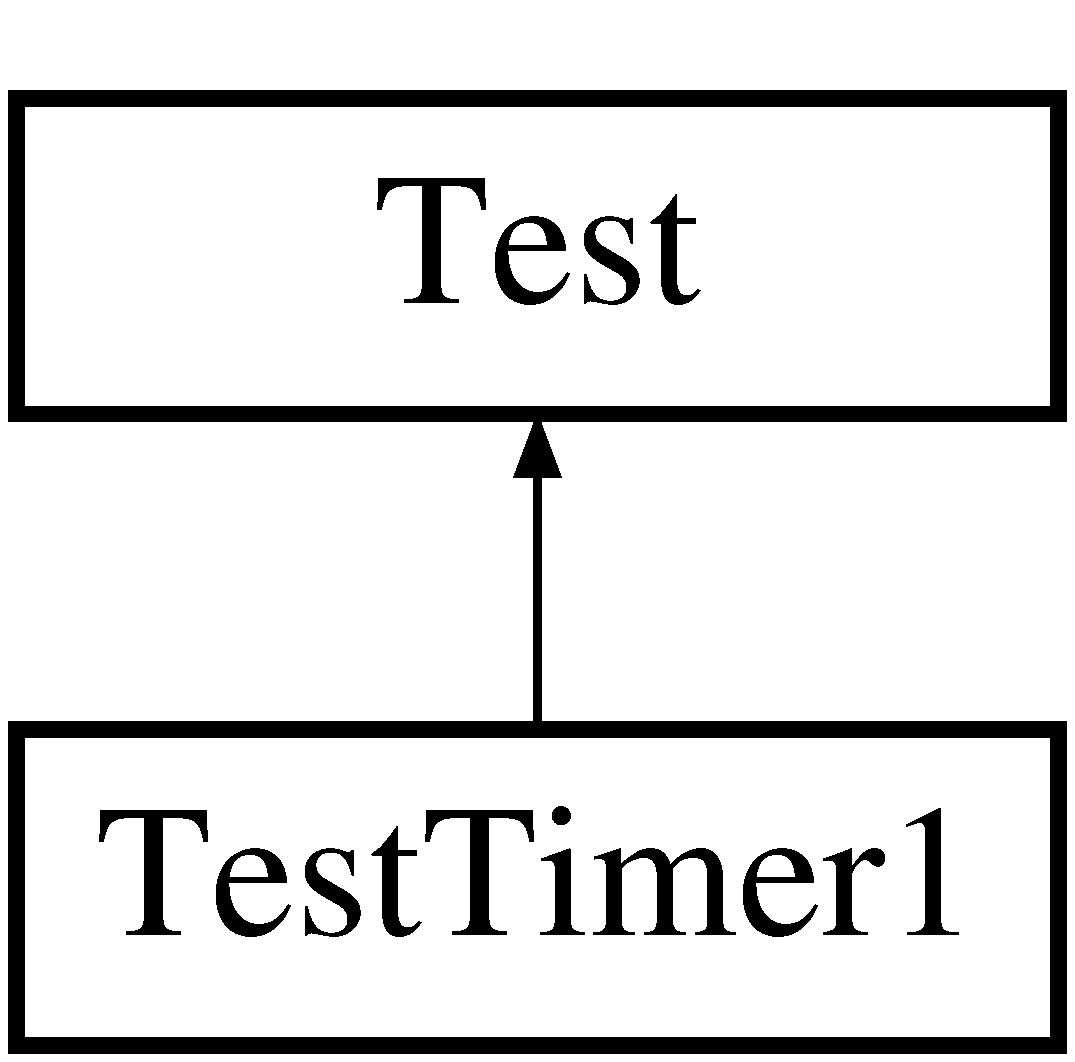
\includegraphics[height=2.000000cm]{class_test_timer1}
\end{center}
\end{figure}
\subsection*{Public Member Functions}
\begin{DoxyCompactItemize}
\item 
\mbox{\Hypertarget{class_test_timer1_a4d7cf69c616454c22965c8ab4c66f2db}\label{class_test_timer1_a4d7cf69c616454c22965c8ab4c66f2db}} 
void {\bfseries test\+Prescaler} (Timer16\+Bit\+::\+Prescale\+Option prescaler, u8 clock\+Select\+Bits)
\end{DoxyCompactItemize}
\subsection*{Public Attributes}
\begin{DoxyCompactItemize}
\item 
\mbox{\Hypertarget{class_test_timer1_add5d5b6530c9413c76006ecf1298a557}\label{class_test_timer1_add5d5b6530c9413c76006ecf1298a557}} 
u8 {\bfseries control\+Register} = 0
\item 
\mbox{\Hypertarget{class_test_timer1_a558b30afc156a6b059dec60b0865afff}\label{class_test_timer1_a558b30afc156a6b059dec60b0865afff}} 
u8 {\bfseries mask\+Register} = 0
\item 
\mbox{\Hypertarget{class_test_timer1_a8dfc65d3d55a990516eedf2b53b45c4a}\label{class_test_timer1_a8dfc65d3d55a990516eedf2b53b45c4a}} 
u16 {\bfseries compare\+Register} = 0
\item 
\mbox{\Hypertarget{class_test_timer1_a73a86e57155af36771df5355b2caea13}\label{class_test_timer1_a73a86e57155af36771df5355b2caea13}} 
u16 {\bfseries counter\+Register} = 0
\item 
\mbox{\Hypertarget{class_test_timer1_ae95c4709c5e8061b5fe4a4c16e46860e}\label{class_test_timer1_ae95c4709c5e8061b5fe4a4c16e46860e}} 
\mbox{\hyperlink{class_timer1}{Timer1}} {\bfseries timer} = \mbox{\hyperlink{class_timer1}{Timer1}}(control\+Register, mask\+Register, compare\+Register, counter\+Register)
\end{DoxyCompactItemize}


The documentation for this class was generated from the following file\+:\begin{DoxyCompactItemize}
\item 
C\+:/\+Development/code/proj/tr2k\+\_\+drum\+\_\+machine/software/drivers/\+Timer1/test/Timer1\+Test.\+cpp\end{DoxyCompactItemize}

\hypertarget{class_timer0}{}\section{Timer0 Class Reference}
\label{class_timer0}\index{Timer0@{Timer0}}
Inheritance diagram for Timer0\+:\begin{figure}[H]
\begin{center}
\leavevmode
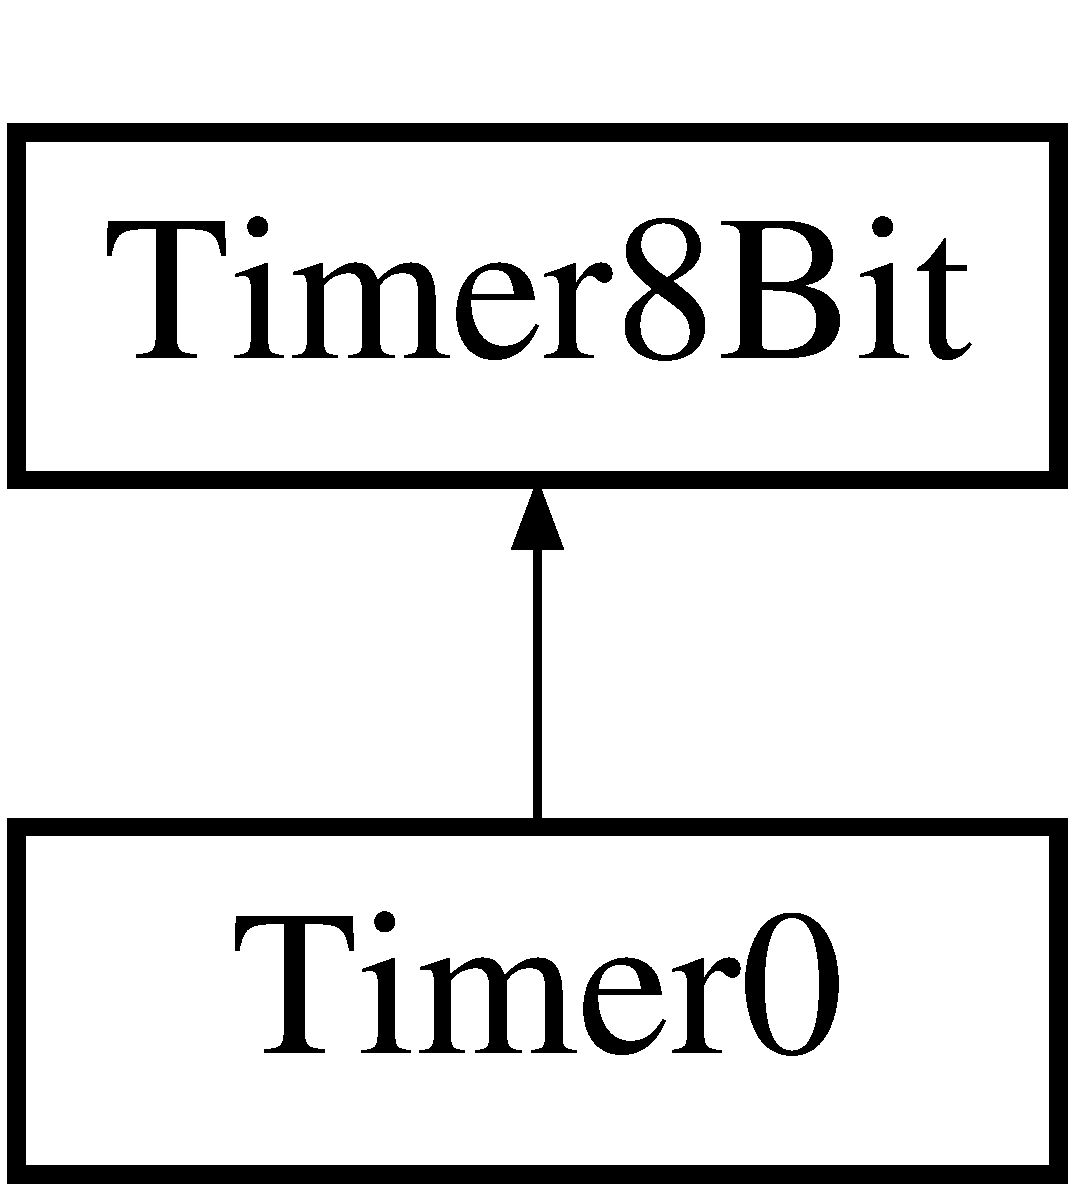
\includegraphics[height=2.000000cm]{class_timer0}
\end{center}
\end{figure}
\subsection*{Public Member Functions}
\begin{DoxyCompactItemize}
\item 
\mbox{\hyperlink{class_timer0_a660c8150e1d5462c7e0cd5b5f173bf5a}{Timer0}} ()
\item 
\mbox{\hyperlink{class_timer0_add6e98a4cf3fcecfe8f2e9372414fbd5}{Timer0}} (u8 \&control\+RegA, u8 \&control\+RegB, u8 \&interrupt\+Mask\+Reg, u8 \&output\+Compare\+Reg, u8 \&counter\+Value\+Reg)
\item 
void \mbox{\hyperlink{class_timer0_a8f0117cda8e82867d58725cf76a73686}{enable\+Periodic\+Interrupts}} ()
\item 
void \mbox{\hyperlink{class_timer0_aaa42d8cd37a0f9f37d42bd4f1f6c91f8}{set\+Prescaler}} (Prescale\+Option prescaler)
\item 
void \mbox{\hyperlink{class_timer0_af19c7f55137a551a3e9ae1c6b15fd4c5}{set\+Period}} (u8 period)
\item 
void \mbox{\hyperlink{class_timer0_a8294e4507ea1b68e090ea77a847257c2}{start}} ()
\item 
void \mbox{\hyperlink{class_timer0_a423cccd0c305d4e552de970b7e71fd0b}{stop}} ()
\item 
void \mbox{\hyperlink{class_timer0_a28a4702cf58fd3cf39ae01e092c0d372}{clear}} ()
\end{DoxyCompactItemize}
\subsection*{Additional Inherited Members}


\subsection{Constructor \& Destructor Documentation}
\mbox{\Hypertarget{class_timer0_a660c8150e1d5462c7e0cd5b5f173bf5a}\label{class_timer0_a660c8150e1d5462c7e0cd5b5f173bf5a}} 
\index{Timer0@{Timer0}!Timer0@{Timer0}}
\index{Timer0@{Timer0}!Timer0@{Timer0}}
\subsubsection{\texorpdfstring{Timer0()}{Timer0()}\hspace{0.1cm}{\footnotesize\ttfamily [1/2]}}
{\footnotesize\ttfamily Timer0\+::\+Timer0 (\begin{DoxyParamCaption}{ }\end{DoxyParamCaption})}

Default constructor, initializes register pointers. \mbox{\Hypertarget{class_timer0_add6e98a4cf3fcecfe8f2e9372414fbd5}\label{class_timer0_add6e98a4cf3fcecfe8f2e9372414fbd5}} 
\index{Timer0@{Timer0}!Timer0@{Timer0}}
\index{Timer0@{Timer0}!Timer0@{Timer0}}
\subsubsection{\texorpdfstring{Timer0()}{Timer0()}\hspace{0.1cm}{\footnotesize\ttfamily [2/2]}}
{\footnotesize\ttfamily Timer0\+::\+Timer0 (\begin{DoxyParamCaption}\item[{u8 \&}]{control\+RegA,  }\item[{u8 \&}]{control\+RegB,  }\item[{u8 \&}]{interrupt\+Mask\+Reg,  }\item[{u8 \&}]{output\+Compare\+Reg,  }\item[{u8 \&}]{counter\+Value\+Reg }\end{DoxyParamCaption})}

Constructor used in tests. 

\subsection{Member Function Documentation}
\mbox{\Hypertarget{class_timer0_a28a4702cf58fd3cf39ae01e092c0d372}\label{class_timer0_a28a4702cf58fd3cf39ae01e092c0d372}} 
\index{Timer0@{Timer0}!clear@{clear}}
\index{clear@{clear}!Timer0@{Timer0}}
\subsubsection{\texorpdfstring{clear()}{clear()}}
{\footnotesize\ttfamily void Timer0\+::clear (\begin{DoxyParamCaption}{ }\end{DoxyParamCaption})\hspace{0.3cm}{\ttfamily [virtual]}}

Clears the timer counter register so that the current period is restarted. 

Implements \mbox{\hyperlink{class_timer8_bit}{Timer8\+Bit}}.

\mbox{\Hypertarget{class_timer0_a8f0117cda8e82867d58725cf76a73686}\label{class_timer0_a8f0117cda8e82867d58725cf76a73686}} 
\index{Timer0@{Timer0}!enable\+Periodic\+Interrupts@{enable\+Periodic\+Interrupts}}
\index{enable\+Periodic\+Interrupts@{enable\+Periodic\+Interrupts}!Timer0@{Timer0}}
\subsubsection{\texorpdfstring{enable\+Periodic\+Interrupts()}{enablePeriodicInterrupts()}}
{\footnotesize\ttfamily void Timer0\+::enable\+Periodic\+Interrupts (\begin{DoxyParamCaption}{ }\end{DoxyParamCaption})}

Enables the timer to generate timer0\+\_\+\+C\+O\+M\+PA interrupts at a frequency determined by the last argument given to \mbox{\hyperlink{class_timer0_af19c7f55137a551a3e9ae1c6b15fd4c5}{Timer0\+::set\+Period()}}. \mbox{\Hypertarget{class_timer0_af19c7f55137a551a3e9ae1c6b15fd4c5}\label{class_timer0_af19c7f55137a551a3e9ae1c6b15fd4c5}} 
\index{Timer0@{Timer0}!set\+Period@{set\+Period}}
\index{set\+Period@{set\+Period}!Timer0@{Timer0}}
\subsubsection{\texorpdfstring{set\+Period()}{setPeriod()}}
{\footnotesize\ttfamily void Timer0\+::set\+Period (\begin{DoxyParamCaption}\item[{u8}]{period }\end{DoxyParamCaption})\hspace{0.3cm}{\ttfamily [virtual]}}

Set the period for the timer before counter rolls back to to 0. If interrupts have been enabled, this period will be the time between each timer0\+\_\+\+C\+O\+M\+PA interrupt. 

Implements \mbox{\hyperlink{class_timer8_bit}{Timer8\+Bit}}.

\mbox{\Hypertarget{class_timer0_aaa42d8cd37a0f9f37d42bd4f1f6c91f8}\label{class_timer0_aaa42d8cd37a0f9f37d42bd4f1f6c91f8}} 
\index{Timer0@{Timer0}!set\+Prescaler@{set\+Prescaler}}
\index{set\+Prescaler@{set\+Prescaler}!Timer0@{Timer0}}
\subsubsection{\texorpdfstring{set\+Prescaler()}{setPrescaler()}}
{\footnotesize\ttfamily void Timer0\+::set\+Prescaler (\begin{DoxyParamCaption}\item[{Prescale\+Option}]{prescaler }\end{DoxyParamCaption})\hspace{0.3cm}{\ttfamily [virtual]}}

Set which prescaler to divide clock source by. 
\begin{DoxyParams}{Parameters}
{\em prescaler} & enum containing legal prescale-\/values. \\
\hline
\end{DoxyParams}


Implements \mbox{\hyperlink{class_timer8_bit}{Timer8\+Bit}}.

\mbox{\Hypertarget{class_timer0_a8294e4507ea1b68e090ea77a847257c2}\label{class_timer0_a8294e4507ea1b68e090ea77a847257c2}} 
\index{Timer0@{Timer0}!start@{start}}
\index{start@{start}!Timer0@{Timer0}}
\subsubsection{\texorpdfstring{start()}{start()}}
{\footnotesize\ttfamily void Timer0\+::start (\begin{DoxyParamCaption}{ }\end{DoxyParamCaption})\hspace{0.3cm}{\ttfamily [virtual]}}

Starts the timer by selecting a prescaled clock source. 

Implements \mbox{\hyperlink{class_timer8_bit}{Timer8\+Bit}}.

\mbox{\Hypertarget{class_timer0_a423cccd0c305d4e552de970b7e71fd0b}\label{class_timer0_a423cccd0c305d4e552de970b7e71fd0b}} 
\index{Timer0@{Timer0}!stop@{stop}}
\index{stop@{stop}!Timer0@{Timer0}}
\subsubsection{\texorpdfstring{stop()}{stop()}}
{\footnotesize\ttfamily void Timer0\+::stop (\begin{DoxyParamCaption}{ }\end{DoxyParamCaption})\hspace{0.3cm}{\ttfamily [virtual]}}

Stops the timer by setting the clock source to none. 

Implements \mbox{\hyperlink{class_timer8_bit}{Timer8\+Bit}}.



The documentation for this class was generated from the following files\+:\begin{DoxyCompactItemize}
\item 
..\textbackslash{}..\textbackslash{}software/drivers/timer0/inc/timer0.\+h\item 
..\textbackslash{}..\textbackslash{}software/drivers/timer0/src/timer0.\+cpp\end{DoxyCompactItemize}

\hypertarget{class_timer1}{}\section{Timer1 Class Reference}
\label{class_timer1}\index{Timer1@{Timer1}}
Inheritance diagram for Timer1\+:\begin{figure}[H]
\begin{center}
\leavevmode
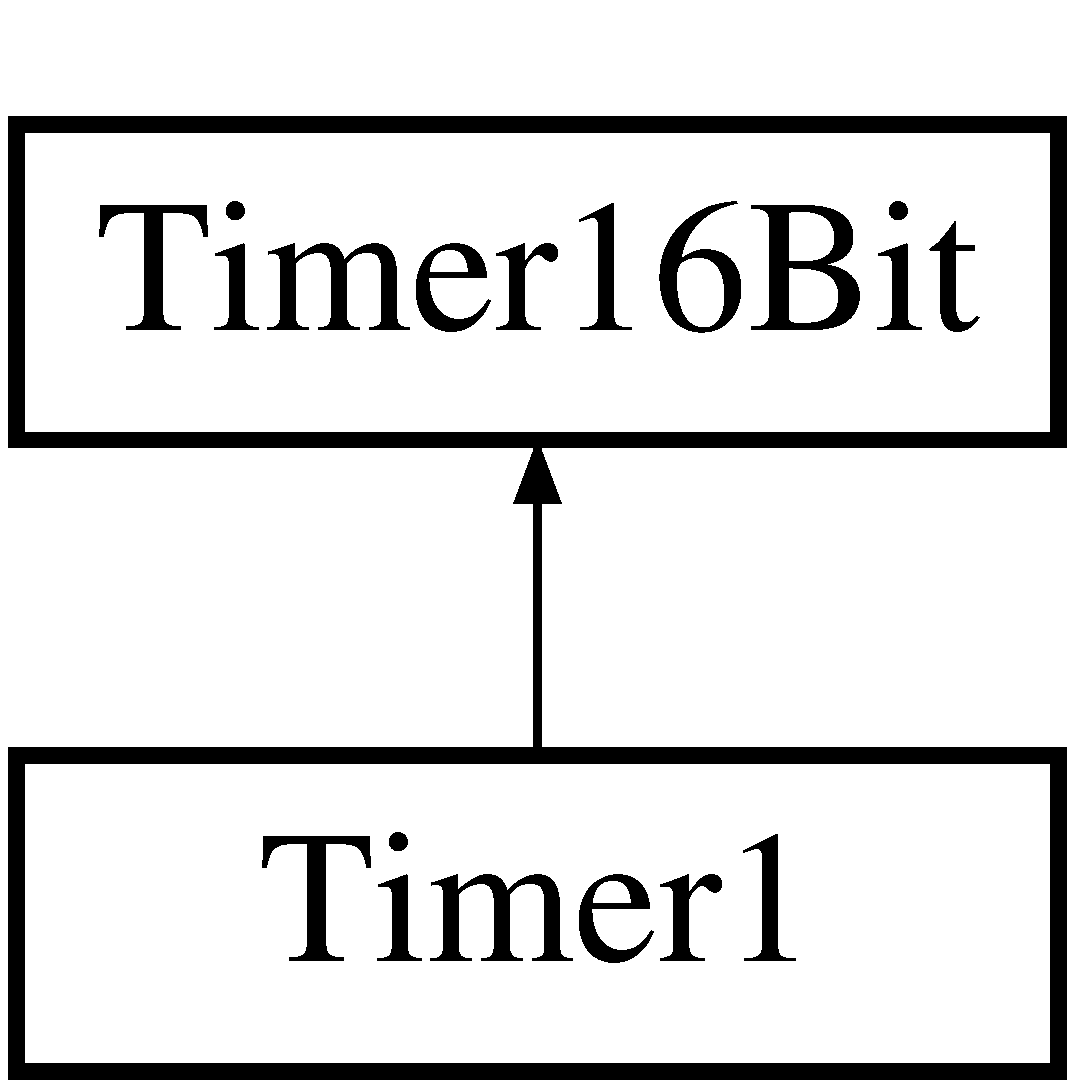
\includegraphics[height=2.000000cm]{class_timer1}
\end{center}
\end{figure}
\subsection*{Public Member Functions}
\begin{DoxyCompactItemize}
\item 
\mbox{\hyperlink{class_timer1_a899c49d4c508ade399a54de9a1a85aeb}{Timer1}} ()
\item 
\mbox{\hyperlink{class_timer1_aef700b65fd584470d6d672ff5df5e6fa}{Timer1}} (u8 \&control\+Reg, u8 \&interrupt\+Mask\+Reg, u16 \&output\+Compare\+Reg, u16 \&counter\+Value\+Reg)
\item 
void \mbox{\hyperlink{class_timer1_adffa570f7391a22de1f6ae1673cd2861}{enable\+Periodic\+Interrupts}} ()
\item 
void \mbox{\hyperlink{class_timer1_a4e841a09f12c8de397440cf6cd74fa4b}{set\+Prescaler}} (Prescale\+Option prescaler)
\item 
void \mbox{\hyperlink{class_timer1_a0aa1eeb582f2a3360f2cb53678c726f9}{set\+Period}} (u16 period)
\item 
void \mbox{\hyperlink{class_timer1_a29031bd6078a40cde7e782628b598035}{start}} ()
\item 
void \mbox{\hyperlink{class_timer1_ace3cab44330dd29aec8182f9a4dfa6f4}{stop}} ()
\item 
void \mbox{\hyperlink{class_timer1_a86a26557d431f334c14524a4c63b2bbe}{clear}} ()
\end{DoxyCompactItemize}
\subsection*{Additional Inherited Members}


\subsection{Constructor \& Destructor Documentation}
\mbox{\Hypertarget{class_timer1_a899c49d4c508ade399a54de9a1a85aeb}\label{class_timer1_a899c49d4c508ade399a54de9a1a85aeb}} 
\index{Timer1@{Timer1}!Timer1@{Timer1}}
\index{Timer1@{Timer1}!Timer1@{Timer1}}
\subsubsection{\texorpdfstring{Timer1()}{Timer1()}\hspace{0.1cm}{\footnotesize\ttfamily [1/2]}}
{\footnotesize\ttfamily Timer1\+::\+Timer1 (\begin{DoxyParamCaption}{ }\end{DoxyParamCaption})}

Default constructor, initializes register pointers. \mbox{\Hypertarget{class_timer1_aef700b65fd584470d6d672ff5df5e6fa}\label{class_timer1_aef700b65fd584470d6d672ff5df5e6fa}} 
\index{Timer1@{Timer1}!Timer1@{Timer1}}
\index{Timer1@{Timer1}!Timer1@{Timer1}}
\subsubsection{\texorpdfstring{Timer1()}{Timer1()}\hspace{0.1cm}{\footnotesize\ttfamily [2/2]}}
{\footnotesize\ttfamily Timer1\+::\+Timer1 (\begin{DoxyParamCaption}\item[{u8 \&}]{control\+Reg,  }\item[{u8 \&}]{interrupt\+Mask\+Reg,  }\item[{u16 \&}]{output\+Compare\+Reg,  }\item[{u16 \&}]{counter\+Value\+Reg }\end{DoxyParamCaption})}

Constructor used in tests. 

\subsection{Member Function Documentation}
\mbox{\Hypertarget{class_timer1_a86a26557d431f334c14524a4c63b2bbe}\label{class_timer1_a86a26557d431f334c14524a4c63b2bbe}} 
\index{Timer1@{Timer1}!clear@{clear}}
\index{clear@{clear}!Timer1@{Timer1}}
\subsubsection{\texorpdfstring{clear()}{clear()}}
{\footnotesize\ttfamily void Timer1\+::clear (\begin{DoxyParamCaption}{ }\end{DoxyParamCaption})\hspace{0.3cm}{\ttfamily [virtual]}}

Clears the timer counter register so that the current period is restarted. 

Implements \mbox{\hyperlink{class_timer16_bit}{Timer16\+Bit}}.

\mbox{\Hypertarget{class_timer1_adffa570f7391a22de1f6ae1673cd2861}\label{class_timer1_adffa570f7391a22de1f6ae1673cd2861}} 
\index{Timer1@{Timer1}!enablePeriodicInterrupts@{enablePeriodicInterrupts}}
\index{enablePeriodicInterrupts@{enablePeriodicInterrupts}!Timer1@{Timer1}}
\subsubsection{\texorpdfstring{enablePeriodicInterrupts()}{enablePeriodicInterrupts()}}
{\footnotesize\ttfamily void Timer1\+::enable\+Periodic\+Interrupts (\begin{DoxyParamCaption}{ }\end{DoxyParamCaption})}

Enables the timer to generate T\+I\+M\+E\+R1\+\_\+\+C\+O\+M\+PA interrupts at a frequency determined by the last argument given to \mbox{\hyperlink{class_timer1_a0aa1eeb582f2a3360f2cb53678c726f9}{Timer1\+::set\+Period()}}. \mbox{\Hypertarget{class_timer1_a0aa1eeb582f2a3360f2cb53678c726f9}\label{class_timer1_a0aa1eeb582f2a3360f2cb53678c726f9}} 
\index{Timer1@{Timer1}!setPeriod@{setPeriod}}
\index{setPeriod@{setPeriod}!Timer1@{Timer1}}
\subsubsection{\texorpdfstring{setPeriod()}{setPeriod()}}
{\footnotesize\ttfamily void Timer1\+::set\+Period (\begin{DoxyParamCaption}\item[{u16}]{period }\end{DoxyParamCaption})\hspace{0.3cm}{\ttfamily [virtual]}}

Set the period for the timer before counter rolls back to to 0. If interrupts have been enabled, this period will be the time between each T\+I\+M\+E\+R1\+\_\+\+C\+O\+M\+PA interrupt. 

Implements \mbox{\hyperlink{class_timer16_bit}{Timer16\+Bit}}.

\mbox{\Hypertarget{class_timer1_a4e841a09f12c8de397440cf6cd74fa4b}\label{class_timer1_a4e841a09f12c8de397440cf6cd74fa4b}} 
\index{Timer1@{Timer1}!setPrescaler@{setPrescaler}}
\index{setPrescaler@{setPrescaler}!Timer1@{Timer1}}
\subsubsection{\texorpdfstring{setPrescaler()}{setPrescaler()}}
{\footnotesize\ttfamily void Timer1\+::set\+Prescaler (\begin{DoxyParamCaption}\item[{Prescale\+Option}]{prescaler }\end{DoxyParamCaption})\hspace{0.3cm}{\ttfamily [virtual]}}

Set which prescaler to divide clock source by. 
\begin{DoxyParams}{Parameters}
{\em prescaler} & enum containing legal prescale-\/values. \\
\hline
\end{DoxyParams}


Implements \mbox{\hyperlink{class_timer16_bit}{Timer16\+Bit}}.

\mbox{\Hypertarget{class_timer1_a29031bd6078a40cde7e782628b598035}\label{class_timer1_a29031bd6078a40cde7e782628b598035}} 
\index{Timer1@{Timer1}!start@{start}}
\index{start@{start}!Timer1@{Timer1}}
\subsubsection{\texorpdfstring{start()}{start()}}
{\footnotesize\ttfamily void Timer1\+::start (\begin{DoxyParamCaption}{ }\end{DoxyParamCaption})\hspace{0.3cm}{\ttfamily [virtual]}}

Starts the timer by selecting a prescaled clock source. 

Implements \mbox{\hyperlink{class_timer16_bit}{Timer16\+Bit}}.

\mbox{\Hypertarget{class_timer1_ace3cab44330dd29aec8182f9a4dfa6f4}\label{class_timer1_ace3cab44330dd29aec8182f9a4dfa6f4}} 
\index{Timer1@{Timer1}!stop@{stop}}
\index{stop@{stop}!Timer1@{Timer1}}
\subsubsection{\texorpdfstring{stop()}{stop()}}
{\footnotesize\ttfamily void Timer1\+::stop (\begin{DoxyParamCaption}{ }\end{DoxyParamCaption})\hspace{0.3cm}{\ttfamily [virtual]}}

Stops the timer by setting the clock source to none. 

Implements \mbox{\hyperlink{class_timer16_bit}{Timer16\+Bit}}.



The documentation for this class was generated from the following files\+:\begin{DoxyCompactItemize}
\item 
C\+:/\+Development/code/proj/tr2k\+\_\+drum\+\_\+machine/software/drivers/\+Timer1/inc/Timer1.\+h\item 
C\+:/\+Development/code/proj/tr2k\+\_\+drum\+\_\+machine/software/drivers/\+Timer1/src/Timer1.\+cpp\end{DoxyCompactItemize}

\hypertarget{class_timer16_bit}{}\section{Timer16\+Bit Class Reference}
\label{class_timer16_bit}\index{Timer16\+Bit@{Timer16\+Bit}}
Inheritance diagram for Timer16\+Bit\+:\begin{figure}[H]
\begin{center}
\leavevmode
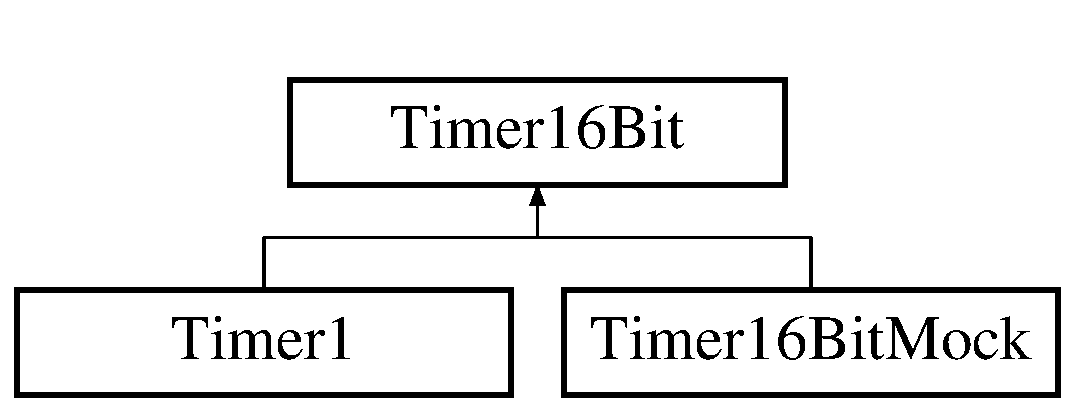
\includegraphics[height=2.000000cm]{class_timer16_bit}
\end{center}
\end{figure}
\subsection*{Public Types}
\begin{DoxyCompactItemize}
\item 
\mbox{\Hypertarget{class_timer16_bit_ae77570668c50b86c26be7d095490ddb4}\label{class_timer16_bit_ae77570668c50b86c26be7d095490ddb4}} 
enum {\bfseries Prescale\+Option} \{ \newline
{\bfseries \+\_\+1}, 
{\bfseries \+\_\+8}, 
{\bfseries \+\_\+64}, 
{\bfseries \+\_\+256}, 
\newline
{\bfseries \+\_\+1024}
 \}
\end{DoxyCompactItemize}
\subsection*{Public Member Functions}
\begin{DoxyCompactItemize}
\item 
\mbox{\Hypertarget{class_timer16_bit_aee78b64b4e1ebd3a0ac5e671f13715c6}\label{class_timer16_bit_aee78b64b4e1ebd3a0ac5e671f13715c6}} 
virtual void {\bfseries set\+Prescaler} (Prescale\+Option prescaler)=0
\item 
\mbox{\Hypertarget{class_timer16_bit_a7e1d467fc113a127dd77e2df135e872f}\label{class_timer16_bit_a7e1d467fc113a127dd77e2df135e872f}} 
virtual void {\bfseries set\+Period} (u16 period)=0
\item 
\mbox{\Hypertarget{class_timer16_bit_a7b26f468974c9da8d96c43f920bda96e}\label{class_timer16_bit_a7b26f468974c9da8d96c43f920bda96e}} 
virtual void {\bfseries start} ()=0
\item 
\mbox{\Hypertarget{class_timer16_bit_abc261659bd9a3b0499e56352dbc37bc3}\label{class_timer16_bit_abc261659bd9a3b0499e56352dbc37bc3}} 
virtual void {\bfseries stop} ()=0
\item 
\mbox{\Hypertarget{class_timer16_bit_a24ab7f6d22dd9af3ad60c7b3472a62a0}\label{class_timer16_bit_a24ab7f6d22dd9af3ad60c7b3472a62a0}} 
virtual void {\bfseries clear} ()=0
\end{DoxyCompactItemize}


The documentation for this class was generated from the following file\+:\begin{DoxyCompactItemize}
\item 
..\textbackslash{}..\textbackslash{}software/hal/if/timer16bit.\+h\end{DoxyCompactItemize}

\hypertarget{class_timer16_bit_mock}{}\section{Timer16\+Bit\+Mock Class Reference}
\label{class_timer16_bit_mock}\index{Timer16\+Bit\+Mock@{Timer16\+Bit\+Mock}}
Inheritance diagram for Timer16\+Bit\+Mock\+:\begin{figure}[H]
\begin{center}
\leavevmode
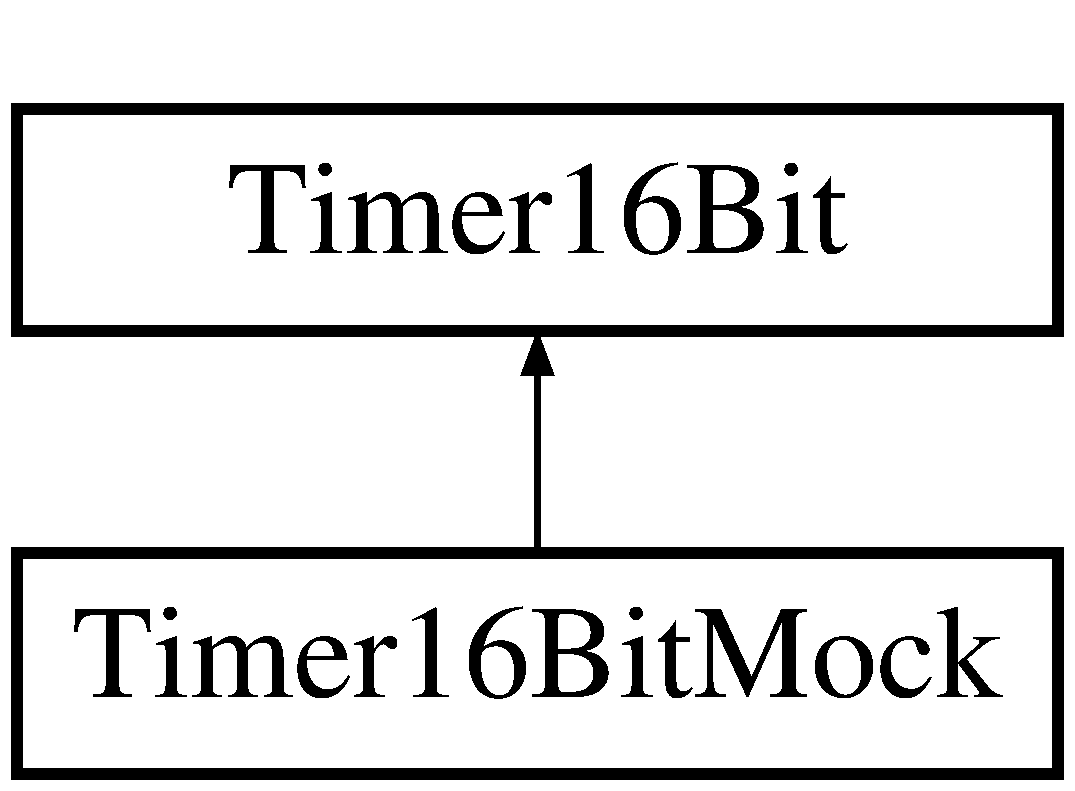
\includegraphics[height=2.000000cm]{class_timer16_bit_mock}
\end{center}
\end{figure}
\subsection*{Public Member Functions}
\begin{DoxyCompactItemize}
\item 
\mbox{\Hypertarget{class_timer16_bit_mock_a8272ab29daf94144c15f64c785e9026c}\label{class_timer16_bit_mock_a8272ab29daf94144c15f64c785e9026c}} 
{\bfseries M\+O\+C\+K\+\_\+\+M\+E\+T\+H\+O\+D1} (set\+Prescaler, void(Timer16\+Bit\+::\+Prescale\+Option prescaler))
\item 
\mbox{\Hypertarget{class_timer16_bit_mock_a0a9dcbb8771b9f12575805ed70e8ae98}\label{class_timer16_bit_mock_a0a9dcbb8771b9f12575805ed70e8ae98}} 
{\bfseries M\+O\+C\+K\+\_\+\+M\+E\+T\+H\+O\+D1} (set\+Period, void(u16 period))
\item 
\mbox{\Hypertarget{class_timer16_bit_mock_a574476d845314c4d19383c824a49b328}\label{class_timer16_bit_mock_a574476d845314c4d19383c824a49b328}} 
{\bfseries M\+O\+C\+K\+\_\+\+M\+E\+T\+H\+O\+D0} (start, void())
\item 
\mbox{\Hypertarget{class_timer16_bit_mock_a8a66e1fe5e8897588b5490c847251e95}\label{class_timer16_bit_mock_a8a66e1fe5e8897588b5490c847251e95}} 
{\bfseries M\+O\+C\+K\+\_\+\+M\+E\+T\+H\+O\+D0} (stop, void())
\item 
\mbox{\Hypertarget{class_timer16_bit_mock_aac6363ec6022b18cc5a612b56ef3573c}\label{class_timer16_bit_mock_aac6363ec6022b18cc5a612b56ef3573c}} 
{\bfseries M\+O\+C\+K\+\_\+\+M\+E\+T\+H\+O\+D0} (clear, void())
\end{DoxyCompactItemize}
\subsection*{Additional Inherited Members}


The documentation for this class was generated from the following file\+:\begin{DoxyCompactItemize}
\item 
..\textbackslash{}..\textbackslash{}software/hal/if/mock/timer16bitmock.\+h\end{DoxyCompactItemize}

\hypertarget{class_timer8_bit}{}\section{Timer8\+Bit Class Reference}
\label{class_timer8_bit}\index{Timer8\+Bit@{Timer8\+Bit}}
Inheritance diagram for Timer8\+Bit\+:\begin{figure}[H]
\begin{center}
\leavevmode
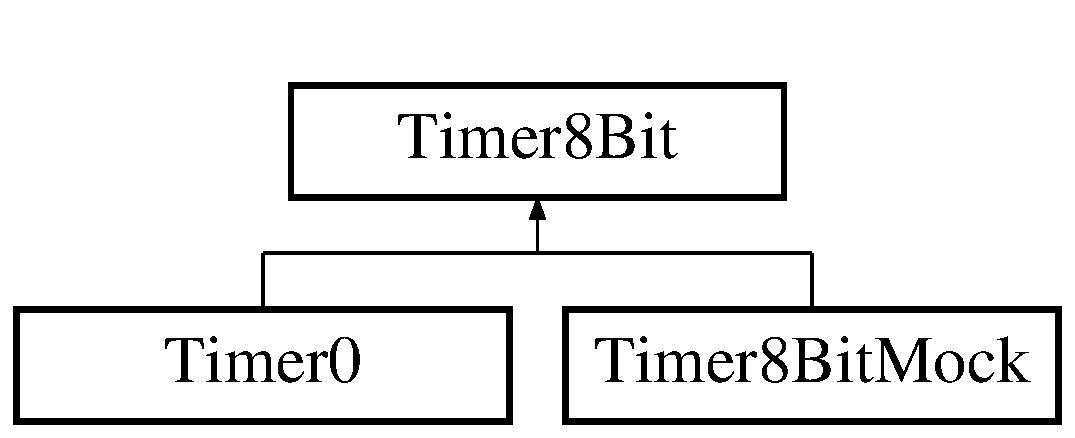
\includegraphics[height=2.000000cm]{class_timer8_bit}
\end{center}
\end{figure}
\subsection*{Public Types}
\begin{DoxyCompactItemize}
\item 
\mbox{\Hypertarget{class_timer8_bit_a6ce4007894d75d11e1c42272ce02e300}\label{class_timer8_bit_a6ce4007894d75d11e1c42272ce02e300}} 
enum {\bfseries Prescale\+Option} \{ \newline
{\bfseries \+\_\+1}, 
{\bfseries \+\_\+8}, 
{\bfseries \+\_\+64}, 
{\bfseries \+\_\+256}, 
\newline
{\bfseries \+\_\+1024}
 \}
\end{DoxyCompactItemize}
\subsection*{Public Member Functions}
\begin{DoxyCompactItemize}
\item 
\mbox{\Hypertarget{class_timer8_bit_a25936cc143d3a691c6b4af8e8101fb2e}\label{class_timer8_bit_a25936cc143d3a691c6b4af8e8101fb2e}} 
virtual void {\bfseries set\+Prescaler} (Prescale\+Option prescaler)=0
\item 
\mbox{\Hypertarget{class_timer8_bit_ab180e7c393b4ba33a689de92e6ca3405}\label{class_timer8_bit_ab180e7c393b4ba33a689de92e6ca3405}} 
virtual void {\bfseries set\+Period} (u8 period)=0
\item 
\mbox{\Hypertarget{class_timer8_bit_adb347e6c1160be1766cd73c6c8940515}\label{class_timer8_bit_adb347e6c1160be1766cd73c6c8940515}} 
virtual void {\bfseries start} ()=0
\item 
\mbox{\Hypertarget{class_timer8_bit_a85d81aff44c77f38282172a6f89986ce}\label{class_timer8_bit_a85d81aff44c77f38282172a6f89986ce}} 
virtual void {\bfseries stop} ()=0
\item 
\mbox{\Hypertarget{class_timer8_bit_a0889614f99eb7ee2470e822ef58ca83d}\label{class_timer8_bit_a0889614f99eb7ee2470e822ef58ca83d}} 
virtual void {\bfseries clear} ()=0
\end{DoxyCompactItemize}


The documentation for this class was generated from the following file\+:\begin{DoxyCompactItemize}
\item 
..\textbackslash{}..\textbackslash{}software/hal/if/timer8bit.\+h\end{DoxyCompactItemize}

\hypertarget{classr2k_1_1vector}{}\section{r2k\+:\+:vector$<$ T, C\+A\+P\+A\+C\+I\+TY $>$ Class Template Reference}
\label{classr2k_1_1vector}\index{r2k\+::vector$<$ T, C\+A\+P\+A\+C\+I\+T\+Y $>$@{r2k\+::vector$<$ T, C\+A\+P\+A\+C\+I\+T\+Y $>$}}
Inheritance diagram for r2k\+:\+:vector$<$ T, C\+A\+P\+A\+C\+I\+TY $>$\+:\begin{figure}[H]
\begin{center}
\leavevmode
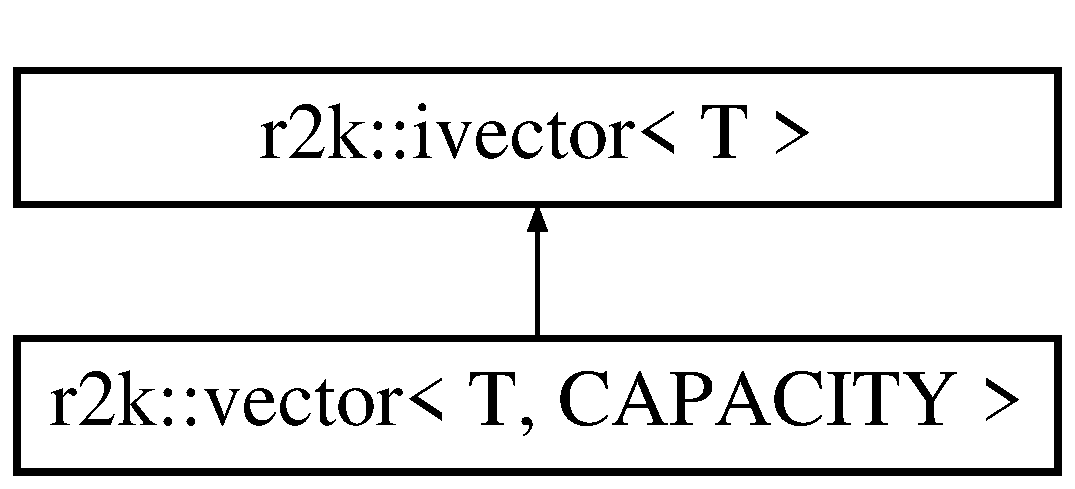
\includegraphics[height=2.000000cm]{classr2k_1_1vector}
\end{center}
\end{figure}
\subsection*{Public Types}
\begin{DoxyCompactItemize}
\item 
\mbox{\Hypertarget{classr2k_1_1vector_a9739a9c18db0500ee97ba4070c9b01cf}\label{classr2k_1_1vector_a9739a9c18db0500ee97ba4070c9b01cf}} 
using {\bfseries value\+\_\+type} = T
\item 
\mbox{\Hypertarget{classr2k_1_1vector_ac0124e2cc6a974eed52ffb62de966b5f}\label{classr2k_1_1vector_ac0124e2cc6a974eed52ffb62de966b5f}} 
using {\bfseries iterator} = T $\ast$
\item 
\mbox{\Hypertarget{classr2k_1_1vector_aba7ed5b7b6e16ff08a8a0e85fe3a9ef8}\label{classr2k_1_1vector_aba7ed5b7b6e16ff08a8a0e85fe3a9ef8}} 
using {\bfseries reference} = T \&
\item 
\mbox{\Hypertarget{classr2k_1_1vector_a9cb5351b24fb72b7841fe05f5bf3911b}\label{classr2k_1_1vector_a9cb5351b24fb72b7841fe05f5bf3911b}} 
using {\bfseries const\+\_\+reference} = const T \&
\end{DoxyCompactItemize}
\subsection*{Public Member Functions}
\begin{DoxyCompactItemize}
\item 
\mbox{\Hypertarget{classr2k_1_1vector_a2d34a926326d09caf04e2f9fef3c7639}\label{classr2k_1_1vector_a2d34a926326d09caf04e2f9fef3c7639}} 
{\bfseries vector} (std\+::initializer\+\_\+list$<$ T $>$ list)
\item 
\mbox{\Hypertarget{classr2k_1_1vector_ad97dcdfbffc7861b98db53a989e5ef1b}\label{classr2k_1_1vector_ad97dcdfbffc7861b98db53a989e5ef1b}} 
iterator {\bfseries begin} () final
\item 
\mbox{\Hypertarget{classr2k_1_1vector_a4ec92e257ec07dd3dcc6ad7dea48e38f}\label{classr2k_1_1vector_a4ec92e257ec07dd3dcc6ad7dea48e38f}} 
iterator {\bfseries end} () final
\item 
\mbox{\Hypertarget{classr2k_1_1vector_adc409c3e3abec361aed5e6b84c75c672}\label{classr2k_1_1vector_adc409c3e3abec361aed5e6b84c75c672}} 
size\+\_\+t {\bfseries size} () const final
\item 
\mbox{\Hypertarget{classr2k_1_1vector_af41940ac9c07142b1c88477ebee14b2d}\label{classr2k_1_1vector_af41940ac9c07142b1c88477ebee14b2d}} 
size\+\_\+t {\bfseries capacity} () const final
\item 
\mbox{\Hypertarget{classr2k_1_1vector_a25615e7c045cfdcc3708748ef652b8d4}\label{classr2k_1_1vector_a25615e7c045cfdcc3708748ef652b8d4}} 
void {\bfseries resize} (size\+\_\+t new\+\_\+size) final
\item 
\mbox{\Hypertarget{classr2k_1_1vector_aba33ce74792e2586fa00f5fe53b417e6}\label{classr2k_1_1vector_aba33ce74792e2586fa00f5fe53b417e6}} 
bool {\bfseries empty} () const final
\item 
\mbox{\Hypertarget{classr2k_1_1vector_a089d03b612cf42f0cf726c2473a1ac67}\label{classr2k_1_1vector_a089d03b612cf42f0cf726c2473a1ac67}} 
reference {\bfseries operator\mbox{[}$\,$\mbox{]}} (size\+\_\+t index) final
\item 
\mbox{\Hypertarget{classr2k_1_1vector_a41640207a0d0a01388ed23bd73dc55a8}\label{classr2k_1_1vector_a41640207a0d0a01388ed23bd73dc55a8}} 
reference {\bfseries back} () final
\item 
\mbox{\Hypertarget{classr2k_1_1vector_a5bb6f8917bf4970ebf6cf3f47b8d6c11}\label{classr2k_1_1vector_a5bb6f8917bf4970ebf6cf3f47b8d6c11}} 
void {\bfseries push\+\_\+back} (const\+\_\+reference val) final
\item 
\mbox{\Hypertarget{classr2k_1_1vector_aa9ccbcf949a833c555dcdb53710b8462}\label{classr2k_1_1vector_aa9ccbcf949a833c555dcdb53710b8462}} 
void {\bfseries pop\+\_\+back} () final
\end{DoxyCompactItemize}


The documentation for this class was generated from the following file\+:\begin{DoxyCompactItemize}
\item 
..\textbackslash{}..\textbackslash{}software/common/inc/r2k/vector.\+h\end{DoxyCompactItemize}

%--- End generated contents ---

% Index
\backmatter
\newpage
\phantomsection
\clearemptydoublepage
\addcontentsline{toc}{chapter}{Index}
\printindex

\end{document}
